\documentclass[12pt]{article}


\usepackage[english]{babel}
\usepackage[utf8x]{inputenc}
\usepackage[T1]{fontenc}
\usepackage{scribe}
\usepackage{listings}
\usepackage{braket}
\usepackage{graphicx} % Required for inserting images
\usepackage{color}
\usepackage{mdframed}

\usepackage{amsmath}
\DeclareMathOperator*{\argmin}{argmin} % no space, limits underneath in displaysdd
\DeclareMathOperator*{\argmax}{argmax} % no space, 

\begin{document}
\title{Classical And Quantum Error Correction Codes}


\author{Hui Jin}
\date{August 2026}


\Lecturer{Hui Jin}
\Contributor{}
\LectureNumber{02}
\LectureDate{DATE}
\LectureTitle{Linear Codes}

\lstset{style=mystyle}

	\MakeScribeTop

%#############################################################
%#############################################################
%#############################################################
%#############################################################
\section{Introduction}
The fundamental problem of channel coding is to encode a stream of message bits into a stream of coded symbols by adding structured redundancy at the transmitter, so that the receiver can use that structure to detect and correct errors. In its simplest form, there is no feedback from the receiver back to the transmitter; this form of channel coding is known as forward error correction.

Forward error correction is the most important technique for fighting the noise present in a communication channel in order to achieve reliable communication. In general, the coded symbols can be binary (taking one of two values) or $q$-ary (taking one of $q$ values, for some integer $q > 2$). In the early days of coding theory, especially in algebraic coding, $q$-ary symbols enabled important coding schemes such as Reed-Solomon codes. However, modern coding methods -- codes defined on sparse graphs, like Low Density Parity Check (LDPC) codes or turbo-like codes -- are usually binary. This does not limit the use of high-order modulation formats in practice: we simply group several coded bits together and map each group onto a modulation symbol before transmission. As a result, $q$-ary symbols have become less central to the theory. In this class we therefore discuss only binary channel coding.

Binary channel coding takes place over the binary field \(GF(2) = \{0, 1\}\): a set of two elements with addition and multiplication defined so that all the usual algebraic rules (associativity, distributivity, etc.) still hold. The only surprising rule is how addition works: \(1 + 1 = 0\). Concretely, this means addition in \(GF(2)\) is the same as the XOR (exclusive-or) operation on bits, and every ``sum'' in this chapter should be read as addition modulo \(2\).

In this chapter, we first discuss various  noisy channel models and two simple coding schemes, the repetition code and the \((7,4)\) Hamming code. Using these two examples, we show the basic concepts such as encoding, decoding. Then we venture into a general framework of block linear codes, the generator matrix for encoding, the parity check matrix for syndrome calculation, and syndrome decoding. 

\section{Noisy Channels}
We limit ourselves to binary input channels. Note that using binary input is a reasonable assumption in low signal-to-noise regimes, (ie noisy channels), as in this scenario, power efficiency is more important. In high signal-to-noise regimes, higher data rate is more important, so spectrum efficiency is more important and we have to use non-binary inputs. 


Therefore we assume the channel has input \(\{0, 1\}\), and output alphabet \(\Sigma_Y\), where \(\Sigma_Y\) can be discrete or continuous. The channel is modeled by the transition probability function \(p(y|x)\), the probability of receiving symbol \(r\) given that the binary value \(x\) is transmitted. 

\begin{example}
    Binary Symmetric Channel (BSC): the output alphabet \(\Sigma_Y\) is \(\{0, 1\}\) and the transition probabilities are:
\begin{align*}
    p(y=0|x=0) &= p(y=1|x=1) = 1- p \\
    p(y=1|x=0) &= p(y=0|x=1) = p
\end{align*}
\begin{figure}[h]
    \centering
    \includegraphics[width=0.5\textwidth]{Figs/BSC_channel.png}
    \caption{Binary Symmetric Channel. Each transmitted bit is flipped with probability \(p\) and received correctly with probability \(1-p\), independently of the other bits. BSC is a good model for channels dominated by random thermal noise.}
    \label{fig:bsc_channel}
\end{figure}

\end{example}

\begin{example}
    Binary Erasure Channel (BEC): the output alphabet \(\Sigma_Y\)  is \(\{0, \star, 1\}\), where \(\star\) represents an erasure. The transition probability are:
\begin{align*}
p(y=0|0) &= p(1|1) = 1 -p \\
p(\star|0) &= p(\star|1) = p
\end{align*}

\begin{figure}[h]
    \centering
    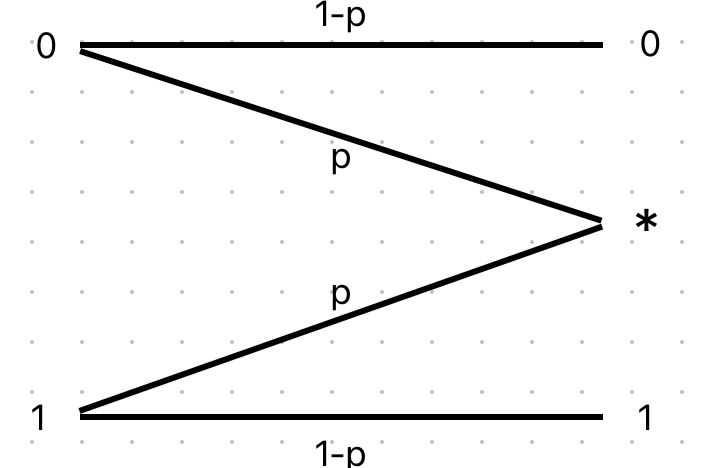
\includegraphics[width=0.5\textwidth]{Figs/BEC_channel.png}
    \caption{Binary Erasure channel. A bit has probability \(p\) erased; otherwise, it is received correctly. BEC is a good model for internet traffic.}
    \label{fig:bec_channel}
\end{figure}

\end{example}

\begin{example}
    Additive White Gaussian Noise Channel (AWGN): here we map bit \(0\) to the transmitted symbol \(+1\) and bit \(1\) to \(-1\) (any fixed mapping between bits and symbols will do). The output value is a Gaussian random variable centered around the transmitted symbol with standard deviation \(\sigma\):
 \begin{align*}
p(y|0) &= \frac{1}{ \sqrt{2\pi\sigma^2}}\; \exp(-(y-1)^2/2\sigma^2) \\
p(y|1) &= \frac{1}{ \sqrt{2\pi\sigma^2}}\; \exp(-(y+1)^2/2\sigma^2) \\
\end{align*}   
Figure~\ref{fig:awgn_channel} depicts the probability distribution given \(\sigma=1\). 

\begin{figure}[h]
    \centering
    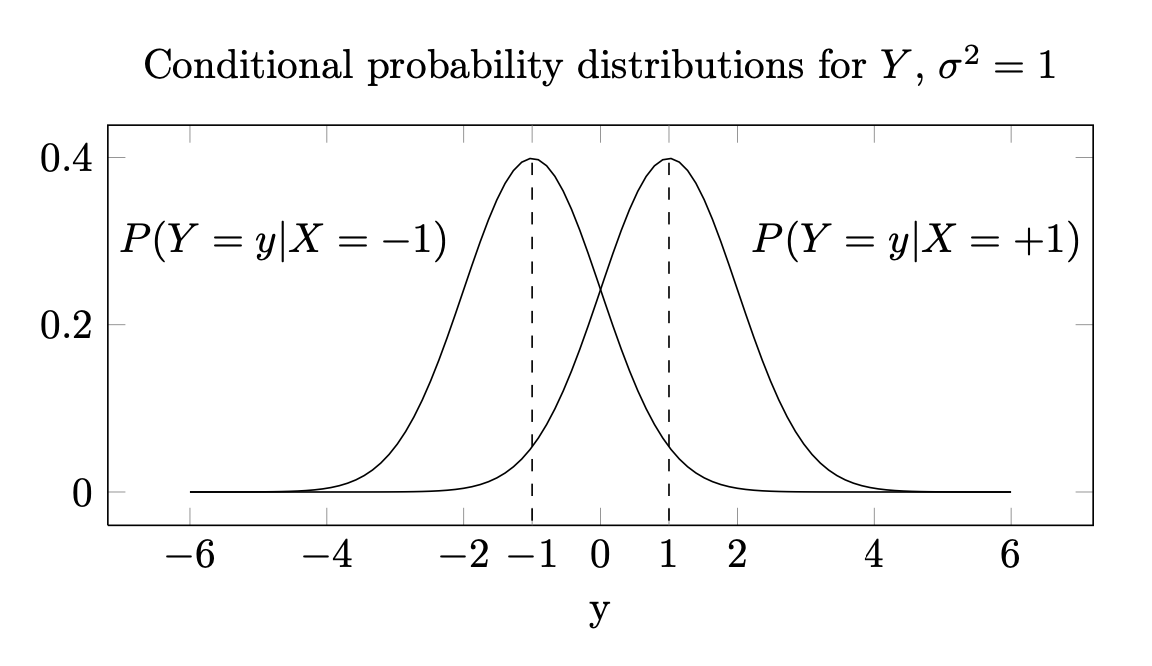
\includegraphics[width=0.5\textwidth]{Figs/BAWGN_pdf.png}
    \caption{Binary Additive White Gaussian Noise channel.}
    \label{fig:awgn_channel}
\end{figure}

The AWGN channel has a continuous output, but a receiver can always fall back to a simple strategy: guess whichever symbol, \(+1\) or \(-1\), is closer to the received value \(y\). This is called making a \emph{hard decision}, and it effectively converts the AWGN channel into a BSC, so it is worth computing the resulting crossover probability \(p\).

By symmetry we may assume the transmitted symbol is \(-1\) and ask for the probability that \(y\) lands closer to \(+1\) than to \(-1\), i.e., that \(y > 0\):
\begin{align*}
    P(-1 \rightarrow +1) &= \frac{1}{ \sqrt{2\pi\sigma^2}}\; \int_{0}^{\infty} \exp(-(y+1)^2/2\sigma^2)\, dy \\
          &= \frac{1}{ \sqrt{2\pi\sigma^2}}\; \int_{1}^{\infty} \exp(-y^2/2\sigma^2)\, dy \\
          &= Q\left(\frac{1}{\sigma}\right)
\end{align*}
where \(Q(\cdot)\) is the standard Gaussian tail probability, i.e., \(Q(x) = P(Z > x)\) for a standard normal random variable \(Z\). This crossover probability \(p = Q(1/\sigma)\) is exactly the BSC parameter that results from hard-decision decoding of the AWGN channel.
\end{example}



\section{Repetition Codes} The simplest coding scheme is a repetition code. 
At the transmitter side, in order to combat noise, we repeat every message bit \(q\) times. Take the example \(q=3\): each message bit is repeated three times. That means we transmit \(000\) if the message bit is \(0\), and transmit \(111\) if the message bit is \(1\). The bits \(000\) and \(111\) are called the code bits. This process of turning \(1\) message bit into \(3\) coded bits is called the encoding process. For a stream of message bits \(10010\), the encoded bit stream will be \(111000000111000\), as illustrated in Figure~\ref{fig:Repeat3}.

\begin{figure}[h]
    \centering    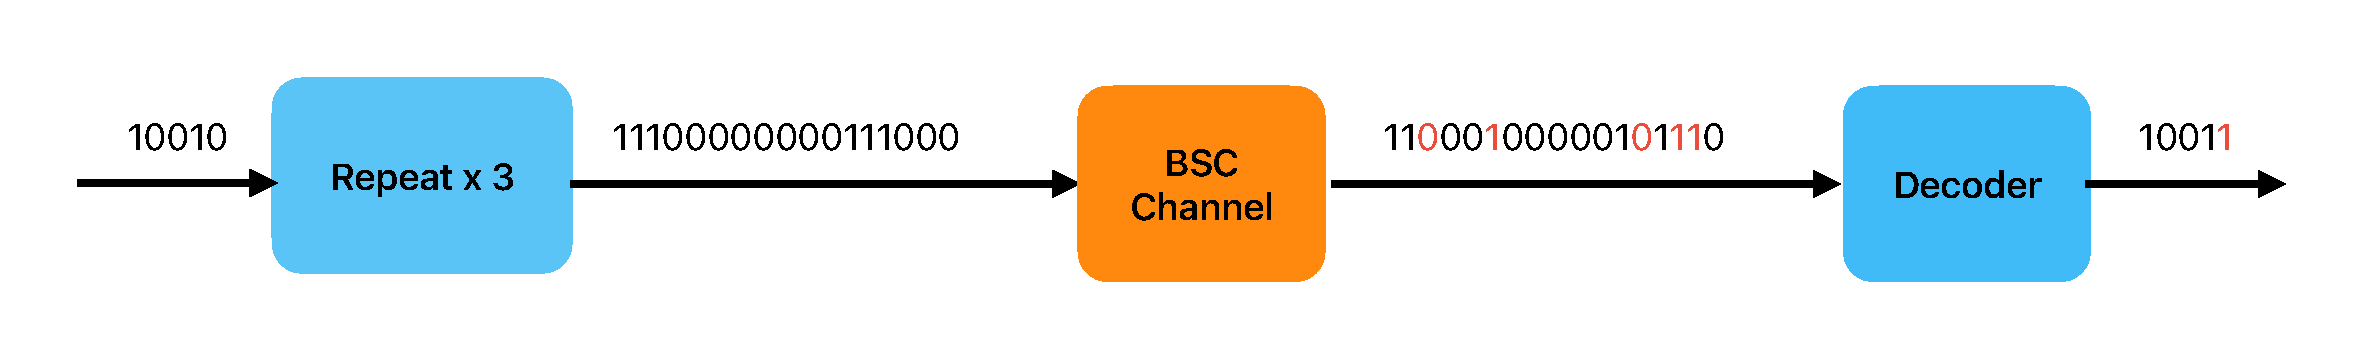
\includegraphics[width=1\textwidth]{Figs/Repeatx3Code.pdf}
    \caption{Encoder and decoder of a Repetition-3 code. The Binary Symmetric Channel (as introduced in the first lecture) has crossover probability \(p\).The decoder is a majority vote decoder for each three coded bits. The decoded message bit has the last bit wrong.}
    \label{fig:Repeat3}
\end{figure}


Let us assume the bits go through a binary symmetric channel with cross-over probability \(p\). Then the receiver, because of the cross-over noise, receives a garbled version, for example, \(110001000101110\), where \(5\) bits are received incorrectly, as indicated by the red color on the bit in Figure~\ref{fig:Repeat3}. The receiver knows that every group of three bits should be identical if there is no noise and it will use that information to decide the correct message bit. This process of using the structured information to infer the right message bit is called the decoding process. 


We first realize the decoding method should decode each message bit separately as there's no information encoded across these bits. So we try to decode the correct message bit given every three coded bits. Assuming the cross-over probability is small, the best decoding method should use a majority vote - the message bit is the bit with the more occurrence. For example, if the received coded bit stream is \(100\), then the message bit is \(0\).

 The message bit will be decoded in error if and only if either two or three of its three copies are flipped by the channel. In the example, the decoded message bit is \(10011\), which we get the last bit wrong. In general, if we use \(P_b^{E}\) denotes the \textbf{bit error probability,} then for repetition code we have:
\begin{align}
    P_b^{E} &= P\{2 \;\text{flips}\} + P\{3 \;\text{flips}\} \nonumber\\
        &= 3p^2(1-p) + p^3 \nonumber \\
        &= 3p^2 - 2p^3. \label{eq:repetitionBER} 
 \end{align}
For \(p < \frac{1}{2}\), the coded bit error probability \(P_b^{E}\) is smaller than \(p\). In fact, for smaller \(p\), the improvement in error probability is significant. 

The improvement of \(P_b^{E}\) over the uncoded system is known as the coding gain. Rigorously, coding gain is defined at a certain error rate and on a particular channel. For example, on the AWGN channel, the difference between the required Signal-to-Noise ratio of a coded system and a uncoded system to achieve a fixed error rate is known as the coding gain for the AWGN channel.   


We can increase the number of repetitions \(q\). In the next we show that as \(q\) goes large, the bit error probability goes to zero. That is we can achieve a reliable communication. Using the argument as in Eq.~(\ref{eq:repetitionBER}) is quite involved; instead we apply the weak law of large numbers.

Let us assume among the \(q\) copies of the message bit, the number of bits get flipped is \(k\) at the receiver,  We will decode correct if \(k < q/2\) by majority vote decoding. Since \(k\) is the number of flips, the weak law of large numbers says the sample mean of the fraction of flips converges to the expected value in probability, or 
\begin{align*}
    \lim_{q} Pr\{|\frac{k}{q} - p| > \epsilon\} = 0.
\end{align*}
 This says as \(q\) goes large, the fraction \(\frac{k}{q}\) converges to \(p\) almost surely. We also know that \(p < \frac{1}{2}\), that means  \(k < q/2\) as \(q\) goes large, which means with probability \(1\) we will be able to decode correctly, in other words,  the decoding error probability goes zero. 



\section{Hamming Code}
Repetition code represents the simplest encoding method; as trivial as it is, it is not efficient. For example for \(q=3\),  every message bit is repeated \(3\) times; the effective rate of information transmission is \(\frac{1}{3}\). Put in a different way, for every information bit, we add \(2\) redundant bits. It can correct 1 flip error. 

Richard Hamming in 1950 introduced a code which could also correct 1-bit error but used less number of redundant (or extra) bits. Hamming code is the first non-trivial error correcting code. Interestingly, Hamming's research happened around the same time as Shannon was inventing the information theory and coding theory. 

The original Hamming code encodes 4 message bits \(x_1, x_2, x_3, x_4\) to 7 coded bits by appending three parity check bits \(x_5, x_6, x_7\):
\begin{align}
 x_5 &= x_2 \oplus x_3 \oplus x_4 \nonumber \\
x_6 &= x_1 \oplus x_2 \oplus x_4 \label{eq:HammingEnc}\\
x_7 &= x_1 \oplus x_3 \oplus x_4 \nonumber 
\end{align}
 
Here \(\oplus\) stands for the XOR operation. We can represent the encoding using a Venn Diagram as depicted in Figure~\ref{fig:HammingVenn}:

\begin{figure}[h]
    \centering    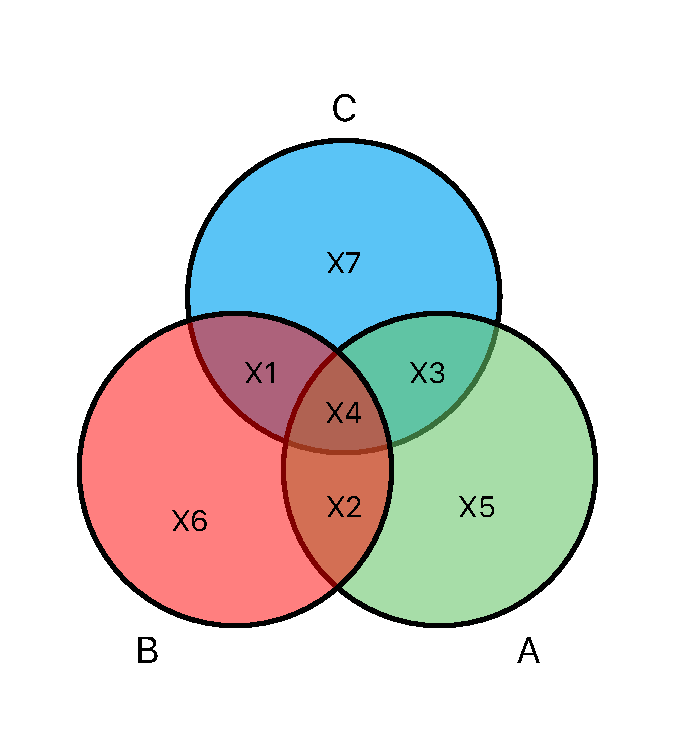
\includegraphics[width=0.6\textwidth]{Figs/HammingVennDiagram.pdf}
    \caption{Venn Diagram of the \((7,4)\) Hamming Code. \(x_1, x_2, x_3, x_4\) are information bits and \(x_5, x_6, x_7\) are parity bits generated. Every circle represents a parity check equation, meaning the sum of the bits in the circle is \(0\).}
    \label{fig:HammingVenn}
\end{figure}




To describe how the receiver recovers the four message bits from the garbled seven-bit codeword, ie the decoding algorithm, we re-write the parity check equations in Eq~\ref{eq:HammingEnc} as 
\begin{align}
   x_2 \oplus x_3 \oplus x_4  \oplus x_5 &= 0 \nonumber \\
 x_1 \oplus x_2 \oplus x_4 \oplus x_6 &= 0 \nonumber \\
 x_1 \oplus x_3 \oplus x_4 \oplus x_7 &= 0  \nonumber
\end{align}
In the Venn diagram Fig~\ref{fig:HammingVenn}, the three parity check equations correspond to circle A, B, and C respectively: all bits in circle A sum up to 0, and so on. 

Now let us form such parity check equations on the received 7-bit vector \(c_1c_2\cdots c_7\) and show that from the result of these three parity checks we are guaranteed to correct one single error:
\begin{align}
   c_2 \oplus c_3 \oplus c_4  \oplus c_5 &= s_1 \label{eq:HamS1} \\
 c_1 \oplus c_2 \oplus c_4 \oplus c_6 &= s_2 \label{eq:HamS2} \\
 c_1 \oplus c_3 \oplus c_4 \oplus c_7 &= s_3  \label{eq:HamS3}
\end{align}

Since there are at most one single error, a satisfying parity check means all bits in the equation is correct; a non-satisfying parity check means exactly one bit in the equation is wrong. From these two facts, we can uniquely determine the flipped bit given the vector \((s_1, s_2, s_3)\).  This fact can be easily seen from the Venn diagram ~\ref{fig:HammingVenn}: if bits in a circle does not sum up to zero, we say that circle is wrong. Then any combination of wrong circles among the three circles uniquely determine a common bit that is included in the wrong circles. If there is at most one single error, this algorithm is guaranteed to succeed. 

\begin{example}
Let us see how we decode the \((7,4)\) Hamming code using a few examples:
\begin{enumerate}
    \item If \((s_1, s_2, s_3) = (1,0,0)\), then the wrong bit only appears in Eq~\ref{eq:HamS1}, or in circle A. That means the bit must be \(c_5\).
    \item If \((s_1, s_2, s_3) = (0,1,1)\), then the wrong bit must participate in both Eqs~(\ref{eq:HamS2},\ref{eq:HamS3}), but not Eq.~\ref{eq:HamS1}. In other words, the bit is only in circle B, and C, but not A. The bit must be \(c_1\).

     \item If \((s_1, s_2, s_3) = (1,1,1)\), then the wrong bit must participate in all these Eqs, that means the bit has to be \(c_4\).
\end{enumerate}
\end{example}


\subsection{Decoding Error Probability of Hamming Code}
Let us consider the error probability that the first message bit \(x_1\) is decoded wrong \(P_{e}^{1}\). (The other bits can be derived similarly). 

Necessarily, but not sufficiently, decoding error happens when there are \(2\) error bits or more among the \(7\) coded bits. We consider the more likely event that there are exactly 2 error bits to get the dominant term. For \(x_1\) to be decoded incorrectly, either \(x_1\) and another bit are flipped, or \(x_1, x_5\) are flipped, or \(x_2, x_3\) are flipped, or \(x_6, x_7\) are flipped. (Refer to the Venn diagram to convince yourself these are the only nine cases for bit \(x_1\) to decode incorrectly.)  There are nine such pairs and this gives the bit error probability 
\begin{align}
    P_{e}^{1} \approx 9 p^2 (1-p)^5. 
\end{align}

Note that this decoding error probability is in the same order as bit error probability of the repetition-\(3\) code Eq.~(\ref{eq:repetitionBER}), at the same time we have \(4\) information bits over every \(7\) coded bits in transmission, a clear advantage. 

\section{Block Codes}
Repetition codes and Hamming codes are two examples of block codes. A block code encode \(k\) information bits to \(n\) coded bits by adding \(n-k\) redundancy bits. There are \(2^k\) codewords among the possible \(2^n\) strings of length-\(n\) binary vector. The essential problem of channel coding is how to effectively select the \(2^k\) codewords such that the we can have good decoding performance while both the encoding and decoding complex is practical.




From our above discussion of repetition codes and \((7,4)\) Hamming code, we know that as it is important for the encoder to make the codewords as far apart as possible as the decoding error depends on the distance between two codewords. A large distance makes it harder for the errors introduced by the channel to cross from a codeword to a nearby distinct codeword. 

For example, for the repetition code with repetition number \(q\), the distance between the two valid codewords is \(q\). So as long as the number of errors is less than \(q/2\), majority vote decoding will recover the correct message bit. So the error probability will decrease as we increase \(q\).

However, a distance property of the codewords imposes a constraint on the number of codewords we can have on the bit-stream of \(n\) bits. Say we want to guarantee a distance property of \(d\), then every codeword excludes all neighboring \(n\)-bit strings within \(d\) distance. That gives an upper bound on the number of codewords. 

We can formalize the question:  Given a minimum distance \(d\) (we shall define it rigorously in the following), what is the maximum number of codewords we can have? This can be understood as picking the maximum number of points on the \(2^n\) lattices so that the distance \(d\) is maintained. In fact, that is exactly the approach we are going to take to derive some heuristic relationship between the number of codewords and the distance property of the codewords.  


Let us first define a few terms which can be used to characterize the properties of codes in general.

\begin{definition}
     The Hamming distance between bit strings \(x\) and \(y\) is defined as the number of positions at which the two strings differ. 

More formally, the Hamming distance \[\Delta(x, y) = |\{i|x_i \neq y_i\}| \]
\end{definition}


\begin{definition}
The Hamming weight of a string \(x\) is defined as the number of non-zero bits in the string.

More formally, the Hamming weight of a string 
\[wt(x) = |\{i|x_i  \neq 0\}|\]
\end{definition} 


\textbf{Remark.} Note that Hamming weight and Hamming distance are directly related: 
\[wt(x-y) = \Delta (x, y).\]


\begin{definition}
A binary error correcting code \(C\) of block length \(n\) is any subset
of \(GF(2)^n\).
    
\end{definition}

\begin{definition}
    A code \(C \subset GF(2)^n\)  is said to have minimum distance \(d(C)\), defined as
\[ d(C) = \min_{c_1 \neq c_2 \in C} \Delta(c1, c2).\]
\end{definition}

Plainly speaking, if \(d(C) = d\), then for every pair of distinct codewords in \(C\), the Hamming distance between them is at least \(d\). And there exists at least two codewords the Hamming distance between them is exactly \(d\).

Given the codeword set \(C\), we can map \(\log_{2}|C|\) message bits uniquely to each of the codeword. Larger number of codewords means more information go through the channel for each codeword. This is the important notion of information code rate:     
\begin{definition}
Information code rate of a binary code \(C\) over with block length \(n\) is defined as 
\[R = \frac{\log_{2}|C|}{n}.\]    
\end{definition}


We sometimes like to normalize the distance of a code to its block length, as we do with rate. To do so, we define the relative distance of a code \(C\), denoted \(\delta(C)\), as the ratio of its distance to its block length:

\[\delta(C) = \frac{d(C)}{n}. \]

\begin{example}
\textbf{Repetition Code}. For a length-\(q\) repetition code, the code rate is \(1/q\) and the minimum distance is \(q\). 
\end{example}

\begin{example}
\textbf{Single Parity Check Code}. The SPC code is generated by adding a redundant parity bit of the other \(n-1\) bits to make a length \(n\) codeword. The code rate is \((n-1)/n\). The parity check code is an example of distance \(2\) code. We can verify that by noticing that all codewords having even weights and there is the all-zero codeword and a codeword with weight \(2\).
\end{example}

\begin{example}
The \((7,4)\) Hamming code discussed earlier is an example of distance \(3\) code. The code rate is \(4/7\). We can verify the distance \(3\) by first showing the difference between two codewords is a codeword, and each codeword has at least hamming weight \(3\). 
\end{example}



\paragraph{Detectable Error} We call a binary error event \(e\) detectable if for any codeword \(c\), the corrupted received vector \(c + e\) is not another codeword. If the code \(C\) has \(d(C)=d\), then any binary error event with weight less than \(d\) is detectable.  

\paragraph{Correctable Error}
We call a binary error event \(e\) correctable if for any codeword \(c\), the corrupted received vector \(c + e\) is closer to another codeword \(c\) than another other codeword. If the code \(C\) has \(d(C)=d\), then any binary error event with weight less than \(\lfloor d/2\rfloor\) is correctable.

We can formalize the above discussion into the following theorem. 
\begin{theorem}
 Consider a binary code \(C\). Then, the following statements are equivalent:
\begin{enumerate}
    \item \(C\) has minimum distance \(2t + 1\);
    \item \(C\) can be used to correct all \(t\) bit errors, but not some \(t+1\) bit errors; 
    \item \(C\) can be used to detect all \(2t\) bit errors, but not some \(2t+1\) bit errors;
    \item \(C\) can be used to correct all \(2t\) erasures, but not some \(2t+1\) erasures.   
\end{enumerate}   
\end{theorem}


\begin{proof}
The proof can be best understood using a geometric visualization. 

Assume statement 1. We can imagine drawing disjoint spheres of radius \(t\) centered at each codeword in \(C\). Such balls are called Hamming balls. Thus, we can uniquely identify the initial codeword from an erroneous string \(s1\) in \(GF(2)^n\) as long as the number of errors is \(\leq t\) by identifying the Hamming ball which contains \(s1\). Additionally, if one or more, but not more than \(2t\) errors occur, then the codeword gets distorted to an erroneous string \(s2\) which must be different from every codeword. Thus such error patterns can be detected. We can also identify up to \(2t\) missing symbols given their positions for any erroneous string \(s3\) by identifying the unique codeword that is consistent with \(s3\).


Assume that statement 1 is false. Thus there exists two codewords \(c_1\) and \(c2\) whose Hamming distance \(d \leq  2t\). 

Consider the midpoint of \(c_1\) and \(c_2\); call it \(x\). The Hamming distance of \(x\) from both \(c_1\) and \(c_2\) is \(\leq t\). 

If \(t\) bit errors are allowed then either \(c_1\) or \(c_2\) could give rise to x. Thus, on the string \(x\) it wouldn’t be possible to correct the errors. Hence \(C\) cannot correct all t symbol errors If \(2t\) symbol errors are allowed then \(c_1\) could give rise to \(c_2\) and thus we cannot be sure that a codeword corresponds to no errors. Hence C cannot detect all \(2t\) symbol errors. If \(2t\) symbols are erased then either \(c_1\) or \(c_2\) could give rise to the same string (take \(c_1\) and erase all positions which are different from \(c_2\)) and thus we cannot correct \(2t\) symbol erasures. 
\end{proof}

\section{Bounds on the size of the Codes}
Obviously, given a fixed \(n\), the higher code rate \(R\) is, the more difficult to have a larger \(d\), or better error protection capability. This is the most fundamental trade-off in codes design.  The following several bounds give a quantitative relationship between code rate and minimum distance. 

\subsection{Singleton Bound}
\begin{theorem}
For a code with minimum distance \(\delta n\), the rate of the code is upper bounded by: 
\begin{align*}
    R \leq 1 - \delta. 
\end{align*}
\end{theorem}

\begin{proof}
We prove that for a code \(C\) to have minimum distance \(d\), then the code size \(|C| \leq 2^{n-d+1}\) by proof by contradiction. If \(|C| > 2^{n-d+1}\), consider the first \(n-d+1\) bits of these codewords, and call it the prefix of a codeword. As there are only \(2^{n-d+1}\) possible prefixes, there are at least two codewords who have identical prefix. But then the distance of these two codewords is at most \(d-1\). Contradiction. 

So \begin{align*}
    |C| &\leq 2^{n-d+1} 
\end{align*}

In the limit \(n\) goes large, we have
\begin{equation}
    R \leq 1- \delta. \label{eq:singletonBound}
\end{equation}
Which says, if minimum distance is a linear fraction of the code block length, then code rate R is upper bounded by \(1-\delta\).    
\end{proof}


The singleton bound is very loose. We can derive much tighter bounds, both in the lower bound and upper bound. Let us consider a much tighter upper bound, the Hamming bound.

\subsection{Hamming Ball}
First, Let us define a Hamming ball \(S_t(c)\) around a codeword \(c\) as the set of length-\(n\) vectors \(e\) such that \(\Delta(e,c) \leq t\), or 
\begin{align*}
    S_t(c) = \{e: \Delta(e,c) \leq t\}
\end{align*}

Let us further define the volume of Hamming ball \(S_t(c)\) as \(Vol(n, t)\), which is independent of \(c\),
\begin{align*}
Vol(n, t) = \sum_{i=0}^{t}  \binom{n}{i}.    
\end{align*}

\begin{lemma} 
Vol(n, pn) is well approximated by \(2^{H(p) n}\), where \(H(x)\) is the binary entropy function, 
\[H(x) = - x \log_2(x) - (1-x) \log_2(1-x).\]

In other words, 
\(log_2 Vol(n, pn) \approx H(p) n.\)
\end{lemma}

\begin{proof}
We have 

\begin{align*}
Vol(n, pn) &= \sum_{i=0}^{np}  \binom{n}{i} \\           & \sim   \binom{n}{np}\\
        &\sim \frac{\sqrt{2\pi n} (n/e)^n} {\sqrt{2\pi np} (np/e)^{np} \sqrt{2\pi n(1-p)} (n(1-p)/e)^{n(1-p)}}  \\
        &\sim \frac{1}{p^{np}(1-p)^{n(1-p)}}  \\
        &= 2^{H(p) n}
\end{align*}
\end{proof}
where in the second approximation we use the Stirling formula: 
\[
m! \sim \sqrt{2\pi m} (m/e)^{m}.
\]

\subsection{Hamming Bound}
 The following Hamming bound improves the singleton bound considerably. In fact, in some cases, it is achievable.

\begin{theorem}
For a code with minimum distance \(\delta n\), the rate of the code is upper bounded by: 
\begin{align*}
    R &\leq 1 - H(\delta). 
\end{align*}
\end{theorem}
We know \(S_t(c_1)\) and \(S_t(c_2)\) cannot be overlapping for every pair of codewords \(c_1, c_2\) if the code is able to correct upto \(t\) errors.   

However, there are only \(2^n\) possible vectors in the whole Hamming space, therefore the number of codewords is upper bounded by:
\begin{align*}
    |C| \cdot Vol(n, t) &\leq 2^n \\
    \log_2 |C| + \log_2 Vol(n, t) &\leq n \\
    R &\leq 1 - H(t/n) 
\end{align*}
This is also called the sphere packing bound due to the argument above. Note that in the limit, \(t/n = \frac{d}{2n} = \delta/2\), we have
\begin{align*}
    R &\leq 1 - H(\delta/2). 
\end{align*}

The Hamming bound makes precise the intuitively obvious fact that error correcting codes can not achieve arbitrarily high rate \(k/n\) while still retaining a linear minimum distance. 

\subsection{Gilbert-Varshmov Bound}
It can be shown that for given \(n, d,\) there exists a linear \([n, k, d]\) code provided
\begin{align*}
2^k \sum_{i=0}^{d-1}\binom{n}{i} < 2^n    
\end{align*}
In the limit of large \(n, k, d,\) and putting \(t = d/2,\) this becomes
\begin{align}
    \frac{k}{n} \geq (1 - H(\frac{2t}{n}))(1-\eta)    \label{eq:GVBound}
\end{align}
where \(\eta \rightarrow 0\)  as \(n \rightarrow \inf\). It can be shown that there exists an infinite sequence of \([n, k, d]\) codes satisfying 
\ref{eq:GVBound} with \(d/n \geq \delta\) if \(\delta < 1/2\). The Gilbert-Varshamov bound necessarily lies below the Hamming bound, but it is an important result because it shows that error correction can be very powerful.

Note that in the limit, \(2t/n = \frac{d}{n} = \delta\), we have
\begin{align*}
    R &\geq 1 - H(\delta). 
\end{align*}

We can plot the singleton, Hamming, and Gilbert-Varshmov bound together. 

\section{Linear Codes}
If we focus on linear codes instead of general block codes, we impose more symmetry and the code structure can be described more succinctly. Surprisingly, the linear constraint does not compromise code performance at all. 

\begin{definition}
If \(C \subset GF(2)^n\) is a subspace of \(GF(2)^n\) then \(C\) is said to be a linear code.
\end{definition}

The linear property makes all codewords symmetric in the sense that from the point of view of any codeword, the relative position of other codewords is identical to that from the all zero codeword.  This is because from any codeword \(c\), the difference between \(c\) and another codeword \(c'\) is exactly identical to the difference between \(c-c'\), which is a codeword, and the all zero codeword. That means the decoding error probability is independent of the codeword, and therefore in decoding analysis or simulation we can assume the all zero codeword is transmitted.


As \(C\) is a subspace, from basic linear algebra theory, there exists a basis \(c_1, c_2, \ldots, c_k\) where \(k\) is the dimension of the subspace. Any codeword \(c\) can be expressed as the linear combination of these basis vectors, ie 
\[c = \sum \alpha_i c_i, \]
where \(\alpha_i \in \{0,1\}.\) 


\subsection{Generator Matrix}
One way to describe the linear code of dimension \(k\) is through the matrix consisting of the \(k\) basis vectors \(c_1, c_2, \cdots, c_k\) as the columns. We call it the generator matrix \(G\). 



\paragraph{Generator matrix} Given an \(n \times k\) generator matrix of full rank \(G\), we define a linear code:
\[ \{Gx \;|\; x \in GF(2)^k \}.\]
 Here we use the convention that codeword is generated by \(Gx\), where \(x\) is a column vector; some books prefer to use \(xG\), where \(x\) is a row vector. Clearly in that case, \(G\) then is a transpose of the \(G\) defined here.


A linear code with block length \(n\), dimension \(k\) and minimum distance \(d\) will be denoted compactly as an \([n, k, d]\) code, where we may omit \(d\) if its value is understood, unknown, or not relevant to the discussion.

The code rate for a \([n, k, d]\) code is simply \(R= k/n\).

\begin{example}
Generator matrix for the repetition\(-3\) code: 
$$G = \begin{bmatrix}
    1 \\
    1 \\
    1
\end{bmatrix}$$
Encoding is \(c = Gx\).
\end{example}

\begin{example}
Generator matrix for the \((7,4)\) Hamming code. 

 
$$G = \begin{bmatrix}
    1 & 0 & 0 & 0\\
    0 & 1 & 0 & 0\\
    0 & 0 & 1 & 0\\
    0 & 0 & 0 & 1\\
    0 & 1 & 1 & 1\\
    1 & 1 & 0 & 1\\
    1 & 0 & 1 & 1
\end{bmatrix}$$
Encoding is \(c = Gx\), mapping a length-4 column vector \(x = [x_1 x_2 x_3 x_4]^T\) to a length-7 vector \(c = G x\) (the operations are done over modulo 2) where \(G\) is the matrix.
\end{example}



The repetition-3 code we discussed earlier is a trivial \([3, 1, 1]\) linear code; the Hamming code we discussed earlier is a linear code and can be represented as \([7, 4, 3]\) code.


As we have seen a linear code \([n, k, d]\) forms a subspace and the generator matrix \(G\) is used to define the subspace uniquely. 




\subsection{Parity Check Matrix}
Another way of defining the subspace \(C\) in \(GF(2)^n\) is to use its null space. The nullspace of \(C\) is defined as all vectors which are orthogonal to every vector in \(C\). This is equivalent to all vectors which are orthogonal to every column vector in the generator matrix \(G\).

Consider the linear equation system \(xG=0\), the solution space of \(x\) has dimension \(n-k\) from basic linear algebra. This is the null space. We denote the null-space as the subspace \(C^{\perp}\). We can call a matrix consisting a basis of supporting vector of this subspace as a generator matrix for \(C^{\perp}\).


Let \(H\) represent of such \((n-k)\times n\) generator matrix of \((C^{\perp})\). The matrix \(H\) is called the parity check matrix and can also be used to uniquely define the code \(C\). In particular, we can define the code \(C\) as all vectors \(c\) satisfying the following condition: 
\[H c = 0.\]

\begin{example}
Parity check matrix for the repetition\(-3\) code: 
$$H = \begin{bmatrix}
    1 & 1 & 0 \\
    1 & 0 & 1 \\
\end{bmatrix}$$
The parity checking means \(Hc = 0\).
\end{example}

\begin{example}
The parity check matrix for the \((7,4)\) Hamming code is:
$$H = \begin{bmatrix}
    0 & 0 & 0 & 1 & 1 & 1 & 1\\
    0 & 1 & 1 & 0 & 0 & 1 & 1\\
    1 & 0 & 1 & 0 & 1 & 0 & 1
\end{bmatrix}$$
We can easily verify each codeword \(c\) in the Hamming code defined by the generator matrix satisfies the equation \(Hc=0\).
\end{example}

One benefit of using the parity check matrix is the minimum distance property of the code is directly linked to the rank of the column vectors of \(H\). This leads to a crude bound on the minimum distance of a linear block code.


\begin{theorem}
The minimum distance of code \(C\) with parity check matrix \(H\) is the smallest number \(d\) such that there exist \(d\) columns of \(H\) which are linearly dependent.
\label{theo:minDistance}
\end{theorem}

\begin{proof}
     The minimum distance of a linear code is equal to the smallest possible weight of a non-zero code. This is true as a linear code must include all zero codeword and the distance property is symmetric across all codewords. Let \(x\) be a non-zero code of smallest weight \(d\). We know that \(Hx = 0\), therefore there exists \(d\) linearly dependent columns of \(H\). Additionally for every set of dependent columns in \(H\) there exists a non-zero code in \(C\) such that \(Hc=0\). Thus, the minimum distance of \(C\) is exactly equal to the size of the smallest linearly dependent column set of \(H\).
\end{proof}

\begin{proposition}
    Let \(C[n,k,d]\) be a code. Then \(d \leq n-k+1\).
\end{proposition}
\begin{proof}
We know the column rank equals to the row rank for any matrix. The rank of the row vectors  of the parity check matrix is at most the number of rows, which is \(n-k\). So any \(n-k+1\) columns are linearly dependent. By theorem~\ref{theo:minDistance}, the minimum distance \(d\) is at most \(n-k+1\).
\end{proof}
    

\subsection{Parity Check Matrix vs Generator Matrix}
The codeword set is the linear combination of the column vectors of the generator matrix \(G\). Without loss of generality, we can permute the rows of \(G\) (which involves changing the ordering of the bits) and with row Gaussian elimination  convert the \(G\) into the following form: 
$$G = \begin{bmatrix}
    I_{k} \\
    P
    \end{bmatrix}
$$
where \(P\) has dimension \(n-k\) by \(k\). 

\begin{theorem}
If the generator matrix \(G\) is in the form: 
$$G = \begin{bmatrix}
    I_{k} \\
    P
    \end{bmatrix}
$$
Then one parity check matrix H is:
\[H = [P \; I_{n-k}]\]
\label{thm:HfromG}
\end{theorem}


\begin{proof}
We check directly that \(H\) annihilates every column of \(G\) (all arithmetic below is over \(GF(2)\)):
\[
HG = [P \; I_{n-k}] \begin{bmatrix} I_k \\ P \end{bmatrix} = P I_k + I_{n-k} P = P + P = 0.
\]
So every codeword \(c = Gx\) satisfies \(Hc = HGx = 0\), meaning \(H\) defines the null space of \(G\); that is, \(H\) is a valid parity check matrix for the code generated by \(G\).
\end{proof}

\section{Dual Code}
We can define a dual code of \(C\), denoted by \(C^{\perp}\) by swapping the role of generator matrix \(G\) and parity check matrix \(H\). That is, we define a code with generator matrix \(G_{dual} = H^T\), where \(H^T\) is the transpose of \(H\). \(H^T\) has dimension \(n \times (n-k)\), therefore the encoding \(x = G_{dual} m\) encodes a \((n-k)\)-bit vector to \(n\)-bit codeword. There are \(2^{n-k}\) codewords. The parity check matrix of the dual code \(H_{dual}\) is \(G^T\). 

Intuitively, this lemma says that if you sum a sign \((-1)^{y\cdot z}\) over every codeword \(y\) in \(C\), the terms either all reinforce each other and add up to the size of the code (when \(z\) belongs to the dual code), or they cancel out perfectly and sum to zero (otherwise). This identity -- relating a linear code and its dual -- will be used later in deriving the decoding capability of CSS codes. 

\begin{lemma}
    Consider a \((n,k)\) linear code \(C\), for a \(n\)-bit vector \(z\), we have  
    \[
     \sum_{y \in C} (-1)^{y \cdot z} =
     \begin{cases}
    |C|, & \text{if } z \in C^{\perp} \\
    0.  & \text{otherwise}
    \end{cases}
    \]
\label{lemma:IdentityDual}
\end{lemma}

\begin{proof}
    If \(z \in C^{\perp}\), then \(y \cdot z = 0\) for any \(y \in C\), so \(S(z) = \sum_{y \in C} (-1)^0 = |C|. \)

    Now consider the non-trial case \(z \notin C^{\perp}\). We know the codespace \(C\) is an abelian group.  The dot product \(\phi_z(y) = y\cdot z\) is a group homomorphism\footnote{The function \(h : G(\star) \rightarrow H(\cdot)\) is a group homomorphism if whenever
\(a \star b = c\)  we have   \(h(a) \cdot h(b) = h(c).\)
In other words, the group H in some sense has a similar algebraic structure as G and the homomorphism h preserves that.
}: \(C \rightarrow Z_2\). This map is surjective when \(z \notin C^{\perp}\), which means that \(K = kernel(\phi_z(y))\) is an index two  subgroup of \(C\). The two cosets - one mapping to \(0\), the other mapping to \(1\) - have the same size. (Another way to see this is that given an element \(s \in C\) where \(\phi_z(s) = 1\), we have for any \(y \in C\) if and only \(\phi_z(y) = 0\) then \(\phi_z(y + s) = 1\), which means the whole set of codewords can be partitioned into two equal size sets whose elements are mapped to \(0\) and \(1\) respectively.) Therefore \(|K|=|C|/2\) and the result follows.

    Alternatively, the non-trial trial case \(z \notin C^{\perp}\) can be explained as the following.

    Assume \(c_0\) is one codeword in \(C\) such that \(c_0 \cdot z = 1\). Then if \(c_1\cdot z = 0\), we have \((c_0 + c_1)\cdot z = 1\);
    if \(c_1\cdot z = 1\), we have \((c_0 + c_1)\cdot z = 0\). That means the whole codewords is partitioned into two groups of equal size such that one group has \(c\cdot z = 0\) and the other group \(c \cdot z =1\) and the result follows.
    This is basically the plain language explanation of the homomorphism proof.
\end{proof}

\subsection{Dual codes of some codes}
\textbf{Dual of the repetition code.} As Exercise 2 below asks you to verify, the dual of the length-\(q\) repetition code is the single parity check code of the same length: its parity check matrix is exactly the \(1\times q\) all-ones generator matrix of the repetition code, and its generator matrix is exactly the repetition code's parity check matrix.

\textbf{Dual of the Hamming code.} The dual of the \((7,4)\) Hamming code is the \([7,3]\) \emph{simplex code}: every nonzero codeword has Hamming weight exactly \(4\), and any two distinct nonzero codewords are at distance \(4\) from each other. (You are encouraged to verify this using the generator and parity check matrices given earlier in this chapter.)

\section{Exercise}
\begin{enumerate}
    \item Prove a code \(C\) with minimum distance \(d\) can correct any \(a\) erasures and \(b\) errors if and only if \(d \geq a + 2b +1\).
    \item Write down the parity check matrix of the dual code for the repetition code? 
    \item The dual code for the repetition code is known as the single parity check code. Determine the number of codewords for a length-n single parity check code. 
    \item Extension from \(GF(2)\) to \(GF(5)\). Assume a codeword is a string of numbers \(x_1x_2\cdots x_n\), where \(x_i \in \{0, 1, 2, 3, 4\}\) and \(x_1 + x_2 + \cdots + x_n = 0 \pmod 5\). Determine the number of such codewords.
    \item Prove theorem \ref{thm:HfromG}.
\end{enumerate}



\newpage 

%
\Lecturer{Hui Jin}
\Contributor{}
\LectureNumber{03}
\LectureDate{DATE}
\LectureTitle{Decoding Linear Block Codes}

\lstset{style=mystyle}

	\MakeScribeTop

%#############################################################
%#############################################################
%#############################################################
%#############################################################
\section{Introduction}
In this chapter, we continue the discussion on linear codes. Linear codes can be defined by the generator matrix, with which the encoding problem seems straightforward. After all, encoding is simply \(Gx\), a matrix vector multiplication. In the worst case, the encoding complexity is quadratic in block length, proportional to the number of ones in the matrix \(G\). The decoding problem, on the other hand, is a completely different beast. 


Decoding error probability is the most important metric, but decoding complexity is also important. Here we introduce some of the heuristic classical decoding algorithms for the block linear codes. We shall see that while optimal decoding method is easy to understand, its complexity is prohibitively large. In fact, the decoding complexity can be exponential in block length in general and thus impractical. In fact, most coding research before 1990s is about finding a good code with practical decoding method. 

\section{Decoding Algorithms}
The decoder's task is to determine the transmitted codeword given the received noisy version of the codeword, by using the structured redundancy introduced by the encoder. Since the channel noise is probabilistic, decoding is probability in nature as well. That is, we can only assert a code will be decoded successfully with certain probability, but never can we assert the decoding is guaranteed to succeed. We say a family of codes is "good" in the sense that the decoding error probability can be made arbitrarily small as the block length becomes large.   

\subsection{Memoryless Channel}
The channel statistics is defined by the transition probability from the transmitted symbol \(c_i\) to the received symbol \(y_i\) 
\[p(y_i|c_i). \] 


Let us assume the received vector is \(\y\), the transmitted codeword is \(\c\). 

 Throughout our class, we assume the channel is memoryless, that is the transition probability of sequential symbols are independent of each other, i.e. there is no inter-symbol dependence. This is true for many channel types, and sometimes achieved through the use of symbol permutations. 
 
 When the channel is memoryless, the probability of receiving the vector \(y\) given codeword \(c\) is transmitted can be factored into:
\[p(y|c) = \Pi_{i} p(y_i|c_i).\]

 
The decoder decides a codeword given the noisy received vector \(y\). We are interested in an optimal solution. There can be multiple criteria for this optimality.

\subsection{Maximum Likelihood Decoder}
The most commonly used decoder is maximum likelihood decoder. 
The maximum likelihood decoder chooses the codeword \(c_{ML}\) such that \(p(y|c)\) is maximized. Or
\[c_{ML} = \argmax_c \: p(y|c) \]


\subsection{Maximum A Posteriori Decoder} The maximum A posteriori (MAP) Decoder chooses the codeword c such that p(c|y) is maximized. 
\[c_{MAP} = \argmax_c \: p(c|y) = \argmax_c p(y|c)p(c) \propto \argmax_{c} \; p(y|c)p(c).\]

Now since usually the probability of transmitting any codeword is uniformly distributed, the MAP decoder is equivalent to the ML decoder. But there is an important distinction. In terms of any single bit, we can get the MAP decision of the single bit, aggregated over all possible codewords. And it turns out this is one of the important techniques in modern coding theory, when iterative decoding is applied.

\subsection{Bit Error Probability vs block error probability}
 If we want to minimize the block error rate, we must chose the most likely codeword,

 \begin{equation*}
x^{B} ( y ) = \argmax_{x} P \{ X = x
|Y =y\}.    
 \end{equation*}
To minimize the bit error rate we must instead return the sequence of most likely bits,
\begin{equation*}
x_{i}^{b} ( y ) = \argmax_{x_i} P \{ X_i = x_i
|Y=y\}.    
\end{equation*}
The reason of these prescriptions is the object of the next exercise.


Exercise 1: Let \((U, V )\) be a pair of discrete random variables. Think of \(U\) as a ‘hidden’ variable and imagine you observe \(V = v\). We want to understand what is the optimal estimate for U given \(V = v\). Show that the function \(v \rightarrow \hat{u}(v)\) that minimizes the error probability \(P(\hat{u}) = P \{U \neq \hat{u}(V )\}\) is given by
\begin{align*}
    \hat{u}(v) = \argmax_u P\{U=u|V=v\}.
\end{align*}

\subsection{Minimum distance decoding}
Given a received vector \(r\), the minimum distance decoding finds the codeword \(c\) such that the Hamming distance \(d(r, c)\) is minimized. It can be done by brute force by going through the set of codewords. Clearly the complexity of this naive decoding is \(2^k\).

In normal channel noise model, as in binary symmetric channel, binary erasure channel, or AWGN channel, a smaller Hamming distance directly translates to higher probability. Therefore, the minimum distance decoding is identical to the maximum likelihood decoding.

\subsection{Syndrome Decoding}
Assume the received vector is \(r = c + e\), a codeword distorted by a binary error vector \(e\). We compute the syndrome \(Hr = H(e+c) = He + Hc = He\). Thus, the syndrome only depends on the error vector and is independent of the codeword.
We can also show that if and only if two error vectors differ by a codeword, they have the same syndrome.

These two facts means that the sets \(e + C\) are partitions of the whole possible received vectors. For each syndrome, we can associate the error vector with the smallest weight. Thus we can make this association a look up table to facilitate decoding.

syndrome table. The syndrome table is an array of pairs: (syndrome, error event). There are in total \(2^{n-k}\)pairs, and the total size is \(2^{n-k}(2n-k)\) bits.
Decoder works as the following: the receiver computes the syndrome s from the received vector r, find the corresponding error vector e, and the decoded message is r+e. This is guaranteed to be the minimum distance decoding.
The decoding complexity is modest as we need only to look up the syndrome, which can be done by a memory index. However the memory grows exponentially with n and it is prohibitively large for reasonably large n.

\begin{example}
We will look at the syndrome decoding for the repetition-\(3\) code.

Syndrome table lists the pair of syndrome and the most likely error vectors. For the repetition code, there are \(4\) such pairs and the following is the syndrome table. 

\begin{center}
\begin{tabular}{ c c  }
00 & 000 \\ 
01 & 001 \\
10 & 010 \\
11 & 100 \\
\end{tabular}
\end{center}

\end{example}

\section{Maximum Likelihood Decoding Error Bound}
In terms of decoding error analysis, which codeword is being transmitted is immaterial. Therefore, we can fix the all zero codeword to be the transmitted codeword.

\subsection{Weight Enumerators}
We define \(A_w\) to be the number of codewords with Hamming weight \(w\) in the block code \(C\). As a function of \(w\), \(A_w\) is also known as the weight numerators of block code \(C\).

\subsection{Block Error}
Given the weight numerator \(A_w\),  we can bound the decoding error probability by the union bound. 

The following theorem shows that \(A_w\) can be used to bound the error probability in an intereting situation, wheren the code is being used on a discrete memoryless channel with a maximum likelihood decoding rule. [Note. Syndrome decoding is maximum likelihood.] 

\begin{theorem}
    Let \(C\) be a binary linear code which is to be used on a DMC with input binary \(\{0, 1\}\) and output alphabet \(\Omega\), a maximum likelihood decoding rules is being used. Then the resulting error probability is bounded by 
    \begin{align*}
        P_E \leq \sum_{w=1}^{n} A_w \gamma ^w, 
    \end{align*}

    where 
    \begin{align}
        \gamma = \sum_{y\in \Omega} \sqrt{p(y|0)p(y|1)}.
    \end{align}
\end{theorem}

The parameter \(\gamma\) is a channel specific constant, known as the Bhattacharya parameter. For the binary erasure channel, 
\begin{align*}
    \gamma_{BEC} = p.
\end{align*}

For the binary symmetric channel, 
\begin{align*}
    \gamma_{BSC} = 2 \sqrt{p(1-p)}.
\end{align*}

For the additive Gaussian channel, with 
\begin{align*}
    p(y|0) &= \frac{1}{\sqrt{2\pi \sigma^2}} e^{-\frac{(y-1)^2}{2\sigma^2}}, \\
    p(y|1) &= \frac{1}{\sqrt{2\pi \sigma^2}} e^{-\frac{(y+1)^2}{2\sigma^2}}
\end{align*}
then, 
\begin{align*}
    \gamma_{AWGN} = e^{\frac{-1}{2\sigma^2}}.
\end{align*}

\begin{proof}
    Let \(C=\{\x_0, \x_1, \cdots, \x_{M-1}\}\), with \(\x_0\) being the all zero codeword. If \(y\) is received, an ML decoder will output a codeword \(\x_i\) for which \(p(\y|\x_i\) is the largest. Because of the code is linear, we can suppose \(\x_0\) is transmitted. The decoder will definitely not output \(\x_i\) if \(p(\y|\x_0) > p(\y|\x_i)\). So if we define \(Y_i = \{\y: p(\y|\x_i) \geq p(\y|\x_0)\}\), it follows that 
    
    \begin{align}
        P_E \leq \sum_{i=1}^{M-1} E_i,
        \label{eq:PEUnion}
    \end{align}

    where 
    \begin{align*}
        E_i = \sum_{\y \in Y_i} p(\y|\x_0).   
    \end{align*}

    Since \(p(\y|\x_i) \geq p(\y|\x_0)\) for \(\y \in Y_i\), 
    we have
    \begin{align}
        E_i &= \sum_{\y \in Y_i} \sqrt{p(\y|\x_0)p(\y|\x_i)} \nonumber \\
        &= \sum_{y \in \Omega^n} \sqrt{p(\y|\x_0)p(\y|\x_i)}
        \label{eq:PEsum}
    \end{align}
    where in the second inequality we simply increase the range in the sum. 

    Now we use the fact that 
    \begin{align*}
        p(\y|\x) = \prod_{k=1}^n p(y_k|x_k)
    \end{align*}, 
    we have by interchanging the order of product and summation in eq.\ref{eq:PEsum}, 
    \begin{align}
        E_i \leq \prod_{k=1}^n \sum_{y \in \Omega} \sqrt{p(y|x_{0k})p(y|x_{ik})} \label{eq:PEsumII}
    \end{align}

    The inner sum in eq.\ref{eq:PEsumII} is clearly \(1\) if \(x_{0k} = x_{ik}\) and \(\gamma\) if \(x_{0k} \neq x_{ik}\). Hence, eq.\ref{eq:PEsumII} reduces to 
    \begin{align}
        E_i \leq \gamma^{d_{H}(\x_0, \x_i)},
        \label{eq:PEUnionTerm}
    \end{align}
    where \(d_{H}(\x_0, \x_i)\) denotes the Hamming distance. Combining eq.\ref{eq:PEUnion} and eq.\ref{eq:PEUnionTerm}, we have
    \begin{align*}
    P_E \leq \sum_{w=1}^n A_w \gamma^{w},
    \end{align*}
    where \(A_w\) is the number of codewords with Hamming distance \(w\) from the all zero codewords, which is number of words of Hamming weight \(w\). 
\end{proof}


As we see, the error is denominated by the smallest \(w\), the minimum distance. 

\section{Complexity of Encoder and Decoder}
Error correcting codes are used in practice to protect messages against noise, so both encoder and decoder complexity are of paramount importance. We have to pay attention to both the algorithmic complexity and implementation complexity. The algorithmic complexity is about the number of operations as a function of the code block length \(n\); the implementation complexity is the hardware complexity, including memory, required to implement the encoder and/or the decoder. 

A competitive coding scheme requires simple encoding and decoding complexity. An exponential algorithmic complexity, like the syndrome decoding, is prohibitive. And a linear encoding complexity is much better than a quadratic encoding complexity.  


For example, computing the Hamming distance  \(d(x,y)\) of two \(n\) bit stream \(x, y\),  takes \(n\) operations.

For another example, given a random generator matrix \(G\), there are on average \(n^2/2\) non-zero entries, so the encoding \(Gx\) takes about \(O(n^2)\) operations. 

A maximum likelihood decoder by brute force search goes over the whole set of codewords  and finds the codeword that gives the maximum probability \(p(y|c)\). This decoding algorithm requires exponential search complexity. 


We will assume that an algorithm of complexity polynomial, is somewhat acceptable, an algorithm of exponent
complexity is “too difficult”.


\newpage 

%
\Lecturer{Hui Jin}
\Contributor{}
\LectureNumber{04}
\LectureDate{DATE}
\LectureTitle{Hamming Codes}

\lstset{style=mystyle}

	\MakeScribeTop

%#############################################################
%#############################################################
%#############################################################
%#############################################################
\section{Introduction}
In describing linear codes in general, we use the example of \((7,4)\) Hamming codes. In this chapter, we describe the general \((2^n-1, 2^n-1-n)\) Hamming code, the first non-trivial code that has many nice properties and some fundamental ideas. We further introduce some other codes related to Hamming code, its dual code, and the simplex code. 


\section{The Hamming Code }

\subsection{The \([7,4, 3]\) Hamming Code}
We defined the \(C0 = [7, 4, 3]\) Hamming code using generator matrix:
$$G = \begin{bmatrix}
    1 & 0 & 0 & 0\\
    0 & 1 & 0 & 0\\
    0 & 0 & 1 & 0\\
    0 & 0 & 0 & 1\\
    0 & 1 & 1 & 1\\
    1 & 0 & 1 & 1\\
    1 & 1 & 0 & 1
\end{bmatrix}$$

\begin{lemma}
    Hamming code can be equivalent defined as using parity check matrix \(H\), as \(C =\{ x \in GF(2)^7 \;|\; H x = 0 \}\) for 
$$H = \begin{bmatrix}
    0 & 0 & 0 & 1 & 1 & 1 & 1\\
    0 & 1 & 1 & 0 & 0 & 1 & 1\\
    1 & 0 & 1 & 0 & 1 & 0 & 1
\end{bmatrix}$$
\end{lemma}

\begin{proof}
    We can easily show that each column vector in \(G\) is in the null space of \(H\). This is equivalent to \(HG\) is an all zero matrix.  
\end{proof}

\paragraph{Correcting One Bit Flip in the Hamming code:} Suppose that \(y\) is a noisy transmission of codeword \(c \in C0\), that is, \(y\) is \(c\) with a single bit flipped. Let us write \(y = c + e_i\), where \(e_i\) is the length-\(7\) vector where bits at all positions except position \(i\) is \(0\) (here the first bit is position \(1\), the second position \(2\), etc, the last position \(7\). Therefore, \(e_1 = (1000000), e_2 = (0100000), \cdots, e_7 = (0000001).\)

Let us discuss the practical way to recover \(c\) from \(y\).

 A naive method would be to flip each bit of \(y\) and see if the resulting vector is in the null space of \(H\), or simply, satisfy each of the three parity check equations. Since the only codeword with distance \(1\) from \(y\) is the codeword \(c\), we will find \(e_i\) by brute force. This requires up to \(7\) matrix multiplications.


A more clever way to correct \(y\) is to simply calculate
\(Hy = H(c + e_i) = Hc + H e_i = H e_i\)
The \(i\)th column of \(H\) is the binary representation of \(i\), and thus this method can recover the value of \(i\) with only a single multiplication.

\subsection{Syndrome Decoding of the Hamming Code}
Syndrome table lists the pair of syndrome and the most likely error vectors. For the \((7,4,3)\) Hamming code, there are \(2^3\) such pairs and the following is the syndrome table. Note every non-zero syndrome (there are \(7\) of them) corresponds to a column in the parity check matrix \(H\), and the error vector is \(I_k\), which is all zero except one \(1\) at index \(k\), corresponding to the column.

\begin{center}
\begin{tabular}{ c c  }
000 & 0000000 \\ 
111 & 0000001 \\
110 & 0000010 \\
101 & 0000100 \\ 
100 & 0001000 \\
011 & 0010000 \\
010 & 0100000 \\
001 & 1000000 \\    
\end{tabular}
\end{center}

This is generalized to the general \([2^r -1, 2^r - r-1, 3]\) Hamming code. Every non-zero syndrome (there are \(2^r - 1\) of them), corresponds to a column in the parity check matrix, and the error event is \(I_k\), which is all zero except one \(1\) at index \(k\), corresponding to the column. 


\subsection{Generalized Hamming Code}
The parity check matrix of the \([7, 4, 3]\) Hamming code consists of columns  of binary representation \(1, 2, \ldots 7.\) We can generalize that to a generalized Hamming code \([2^r - 1, 2^r - r -1, r]\)

Define \(H_r\) to be the \(r \times (2^r-1)\) matrix where column \(i\) of \(H_r\) is the binary representation of \(i\), where \(i\) runs from \(1\) to \(2^{r}-1\). 

This matrix contains column vector \(e_1\) through \(e_r\), corresponding to the binary representations of \(2^0, 2^1, \cdots 2^{r-1}\) respectively, and thus has full rank.

Using \(H_r\) as the parity check matrix, we can define the Hamming code 
\(C_r\) as an \([n=2^r-1, k=2^r - 1 -r]\) binary linear code:

\[C_r =\{ c \in GF(2)^{2^r-1} |H_r c= 0 \}. \]

We would like to know the minimum distance of this code is, but in order to compute that, we will need the following lemma.

\begin{lemma}
    The minimum distance of a linear code is the minimum Hamming weight of a nonzero codeword.
\end{lemma}

\begin{proof}
    Assume \(d(c_1, c_2)\) gives the minimum distance. But this is a linear code, \(c_1 - c_2\) is also a codeword. Therefore \(d(c_1, c_2) = wt(c_1 - c_2)\), the minimum distance is a Hamming weight of a non-zero codeword. The steps are reversible, so the minimum distance of a linear code is the minimum Hamming weight of a non-zero codeword.  
\end{proof} 

Then to know the distance of the Hamming code, we must determine the minimum weight of a nonzero codeword. Since the codewords are defined as the vectors c such that \(Hc = 0\), this is equivalent to determining the size of the smallest linearly dependent set of columns of \(H\). \(H\) does not contain a zero column, nor does it contain two equal columns, so this set must contain at least \(3\) elements. On the other hand, many triples of three columns are linearly dependent. For example, the first three columns of \(H\) represent \(1, 2,\) and \(3\) in binary and sum (mod 2) to zero. This shows that the Hamming code in fact has distance \(3\).

\begin{theorem}
    The Hamming code is the best possible code (in terms of \(k\)) with distance \(3\). In other words, the Hamming code has optimal rate.
\end{theorem}
\begin{proof}
Consider a distance 3 code of block length n with \(2^k\) codewords. Within distance \(1\) of each codeword there are \(n + 1\) different points, \(n\) corresponding to the \(n\) possible bit flips and one corresponding to flipping no bits. There are only \(2^n\) points in the entire space, and thus \(n\) and \(k\) must satisfy
\begin{align*}
2^k (n+1) &\leq 2^n \\
k &\leq n = log_2(n+1)
\end{align*}

implying that The Hamming code \(C_r\) with \(k = 2^r -1 -r\) and \(n=2^r-1\) achieve equality of this bound.
\end{proof}

This bound is simply the special case \(d=3\) for the Hamming bound in the Linear codes chapter.


\paragraph{Perfect codes}
Codes which meet this bound are called perfect codes. Perfect codes are rare. It has been shown that for binary linear codes, the Hamming codes, the trivial code \([n, 1, n]\) code with codewords \(0^n\) and \(1^n\) for odd \(n\), and the Golay code \([23,12]\) are the only perfect codes. 

It turns out this property is almost irrelevant   in modern coding. In other words, in modern coding, we are interested in searching for almost perfect codes. 

\subsection{Dual Code of Hamming Code}

The dual of the Hamming code is a linear code with parameters \([2^r-1, r]\)
with a generator matrix whose rows are all the nonzero \(r\)-bit vectors. This is the Simplex code. If we include the zero row, we obtain the Hadamard code \([2^r, r]\). The Hadamard code is the most redundant possible linear code in which no codeword bit repeats in every codeword.

We saw earlier that the Hamming code has optimal rate, but its relative distance is \(\frac{3}{2^r}\). The \(2^r\)
Hadamard and Simplex codes have the awful rate \(\frac{r}{2^r}\), which goes to zero as r increases, but they
make up for this by having a very large distance:


\begin{proposition}
    The Simplex codes have distance \(\frac{n}{2}\).
\end{proposition}

\section{Hamming vs Simplex Codes}
The comparison between the Hamming and Simplex codes show the two endpoints of the spectrum implied by the Hamming bound. The Hamming code has optimal rate but low relative distance, and the Simplex codes have poor rate but optimal distance. An interesting question is

     Are there codes that have good rate and relative distance?

This is closely related to the channel coding theorem which we will cover in the next lecture.


\section{Tanner Graph of Block Linear Codes}
A really useful way to look at linear codes is by using a Tanner graph. A Tanner graph is a bipartite graph made of two groups of nodes and the edges connecting nodes between the two groups. The first group of nodes, called the variable nodes, represent the bits in the codeword; the second group of nodes, called the check nodes, represent the linear constraint of the bits. Each check node corresponds to a row in the parity check matrix. For example, the Tanner graph of the \((7,4)\) Hamming code is depicted in Figure ~\ref{fig:TannerHamming}
\begin{figure}[h]
    \centering
    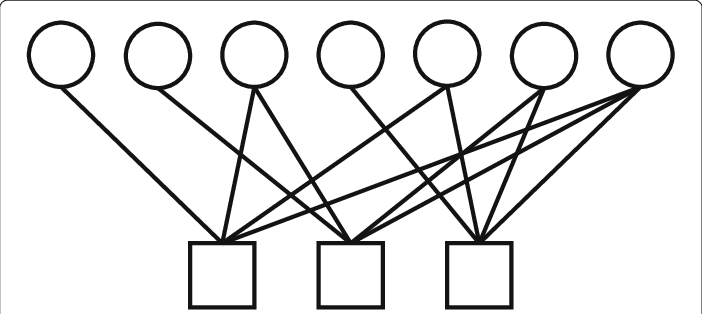
\includegraphics[width=0.5\textwidth]{Figs/Tanner-graph-Hamming.png}
    \caption{Caption}
    \label{fig:TannerHamming}
\end{figure}

$$H = \begin{bmatrix}
    0 & 0 & 0 & 1 & 1 & 1 & 1\\
    0 & 1 & 1 & 0 & 0 & 1 & 1\\
    1 & 0 & 1 & 0 & 1 & 0 & 1
\end{bmatrix}$$

can be \(I_k\), which is all zero except one \(1\) at index \(k\), corresponding to the column.


\newpage 

%
\Lecturer{Hui Jin}
\Contributor{}
\LectureNumber{06}
\LectureDate{DATE}
\LectureTitle{Capacity For Binary Input Memoryless Channel}

\lstset{style=mystyle}

\MakeScribeTop

%#############################################################
%#############################################################
%#############################################################
%#############################################################

\section{Introduction}
In our discussion of block linear codes, we have seen that the tradeoff between the rate of the code, ie \(R= k/n\), and the decoding error probability \(P_e\), is fundamental. On one hand, to achieve reliable communication over a noisy channel, we need to add sufficient redundancy as a funciton of the noise level; on the other hand, the redundancy added reduces the actual information that can be transmitted over. So what is this optimal trade-off, as a function of the noise level present in the communication channel? Since noise is stochastic, we have to state the problem carefully. 

Before Shannon’s 1948 work, people generally assumed that getting reliable communication, i.e. driving the bit error rate \(P_b \rightarrow 0\) requires a vanishing rate. But Shannon in his landmark 1948 paper showed that we do not have to sacrifice rate to communicate reliably. 

\paragraph{Shannon's limit} Shannon’s remarkable theorem on channel coding gives a definitive answer on this trade-off. The theorem identifies when reliable transmission is possible over the stochastic noise models. In particular, for the general framework of noise models, Shannon defined the notion of capacity \(C\), which is a real number such that reliable communication is possible if and only if the rate is less than the capacity of the channel. 

In other words, given a noisy channel with capacity \(C\), if information is transmitted at rate \(R\) for any \(R < C\) , then there exists a coding scheme that guarantees negligible error probability of communication. On the other hand if \(R > C\), then regardless of the chosen coding scheme there will be some message for which the decoding error probability is bounded from below by some constant. 

In this chapter, we will review some of the fundamental concepts in information theory, in the context of a communication channel with noise. We discuss these concepts more relevant to the channel coding: entropy, relative entropy, and mutual information. Then we define the channel capacity, aka Shannon's limit, as the maximum mutual information over the input probability function. For simplicity, we focus on binary input memoryless channels. Then, we will describe the channel capacity for some of the standard binary input noise models. Finally we state Shannon’s theorem, and show a sketch of the proof for the special case of Binary Symmetric Channel.

\section{Information Theory}
\subsection{Entropy Of A Discrete Random Variable}
Suppose \(X\) is a discrete random variable over a finite support set \(\mathcal{X} = \{x_1, x_2, \cdots, x_n\}\). Let \(p_i = P(X=x_i)\) for each \(1 \leq i \leq n\). The entropy of \(X\) is defined as 
\begin{align}
    H(X) = \sum_{x \in \mathcal{X}} p(x) \log \frac{1}{p(x)} = \sum_{i=1}^{n} p_i \log \frac{1}{p_i}.\label{eq:entropy}
\end{align}
We can use any base in the log in the above definition. If we use log in base \(2\), the resulting unit of the entropy is bit; if we use the natural log, then the unit is nat. In our discussion, we use log in base \(2)\) as the default.

The entropy \(H(X)\) of a discrete random variable \(X\) is a measure of the amount of uncertainty associated with the value of \(X\) given its density function. The more uniform the distribution is, the higher the entropy.



\begin{example}
Let \(X\) represents the outcome of a single coin toss of a fair coin. Then \(\mathcal{X} = \{H, T\}\) and \(p_1 = p_2 = \frac{1}{2}\). We have \(H(X) = 1\) bits. 
\end{example}

\begin{example}
    Let \(X\) represents the outcome of a single coin toss of a biased coin, where the probability of getting a head is \(p\) and the probability of get a tail is \(1-p\). Here \[H(X) = -p\log_{2} p - (1-p) \log_{2} (1-p) = H(p)\] bits. 

    The graph of the function \(H(p)\) is shown in Figure~. The figure illustrates some of the basic properties of entropy: first, it is a concave function of \(p\), and it is symmetric, and the uncertainty is maximum when \(p=\frac{1}{2}.\)
\end{example}

\begin{example}
Let \(X\) represents the outcome of a single roll of a fair die. Then \(\mathcal{X} = \{1, 2, 3, 4, 5, 6\}\) and \(p_i = \frac{1}{6}\) for each \(1\leq i \leq 6\). Here we have \(H(X)= \log_{2}(6)\) bits.
\end{example}

\begin{theorem}
Assume \(X\) is a discrete random variable over a finite support set \(\mathcal{X} = \{x_1, x_2, \cdots, x_n\}\). Then 
\[ 0 \leq H(X) \leq \log n.\]
Furthermore, \(H(X)=0\) iff \(p_i=1\) for some \(i\); \(H(X)=\log (n)\) iff \(p_i = 1/n\) for all \(i\).
\end{theorem}

\textbf{Proof:} First in the definition of entropy Eq~\ref{eq:entropy}, each term \(p_i \log \frac{1}{p_i}\) is non-negative, so \(H(x) \geq 0\). Since term \(p_i \log \frac{1}{p_i}\) is zero iff \(p_i = 0\) or \(1\), we have \(H(X)=0\) iff \(p_i=1\) for some \(i\).

For the other direction, we use the fact that \(\log\) function is concave down and apply Jensen's inequality:
\begin{align*}
    H(X) &= \sum_{i=1}^{n} p_i \log \frac{1}{p_i} \\
        &\leq \log (\sum_{i=1}^{n}p_i \frac{1}{p_i}) \\
        &= \log(n).
\end{align*}
For Jensen's inequality to hold equality, all \(p_i\) must be equivalent, which equals to \(\frac{1}{n}\).

\subsection{Joint Entropy}
We now extend the entropy definition to a pair of random variables \(X, Y\). If we treat the pair of random variable \((X,Y)\) as a new random variable \(Z=(X,Y)\), which is a Cartesian product of two random variables, then the entropy of \(Z\) is the joint entropy of the two random variables \(X,\) and \(Y\).

\begin{definition}
    The joint entropy \(H(X,Y)\) of a pair of discrete random variable \(X,Y\) with a joint distribution \(p(x,y)\) is defined as 
    \[ H(X,Y) = -E[\log p(x,y)] = -\sum_{x,y} p(x,y) \log p(x, y).\]
\end{definition}

\begin{theorem}
If \(X, Y\) are two independent random variables, ie \(p(x,y) = p(x)p(y)\), then 
\[H(X,Y) = H(X) + H(Y).\]
\end{theorem}

\subsection{Conditional Entropy} 
The conditional entropy of \(Y\) given \(X\) is defined as
\begin{equation}
H(X|Y) = - E[\log {p(x|y)}] = - \sum_{x \in \mathcal{X}, y \in \mathcal{Y}} p(x,y) \log_{2} p(x|y), \label{eq:CondEntropy}
\end{equation}
where \(\mathcal{X}\) and \(\mathcal{Y}\) denote the support sets of \(X\) and \(Y\). 

Another way to think about \(H(X|Y)\) is to treat \(H(X|Y=y)\) as a random value and \(H(X|Y)\) is the expected value of this random variable. 

\begin{equation}
H(X|Y) = E_y[H(X|Y=y)] = \sum_{y \in \mathcal{Y}} p(x,y) \log_{2} p(x|y), \label{eq:CondEntropy2}
\end{equation}


We will verify that this view gives the same value as the official definition. 


\begin{theorem} (Chain rule)
\begin{equation}
    H(X,Y) = H(X) + H(Y|X).
\end{equation}
\end{theorem}

\begin{proof}
Fundamentally this follows from the well known relationship:
\begin{equation*}
p(x,y) = p(x)p(y|x).
\end{equation*}

Taking logarithm both side, we have 

\begin{align*}
-\log p(x,y) = -\log p(x) - \log p(y|x).
\end{align*}

Therefore, 
\begin{align*}
    H(X,Y) &= - \sum_{x,y} p(x,y) \log p(x,y) \\
           &= - \sum_{x,y} p(x,y) \log p(x) - \sum_{x,y} p(x,y) \log p(y|x)  \\
           &= H(X) + H(Y|X)
\end{align*}

\end{proof}


\subsection{Relative Entropy} 

Entropy of a random variable is a measure of the amount of the information required on the average to describe the random variable; it is a measure of the distribution. 

Relative entropy or Kullback Leibler divergence is a measure of the distance between two distributions \(p(x)\) and \(q(x)\)


\begin{definition}
\begin{equation*}
D(p||q) = \sum_{x} p(x) \log \frac{p(x)}{q(x)}.    
\end{equation*}
\end{definition}

Using relative entropy as a target function is an important technique in machine learning. For example, in image classification, we minimize the the relative entropy between the estimated probability density function and the labeled data density function. 


\subsection{Mutual Information}
The mutual information (MI) of two random variables is a measure of the mutual dependence between the two variables. 

It is defined as
\begin{align}
I(X,Y) &= H(X) - H(X|Y)
\end{align}

In plain language, \(H(X)\) is the uncertainty for the random variable \(X\), \(H(X|Y)\) is the uncertainty for the random variable \(X\) after \(Y\) is known, so \(H(X) - H(X|Y)\) is the information about \(X\) contained in the \(Y\), or the mutual dependence.


Alternatively, the mutual information can be defined as a relative entropy between two distributions on \(X,Y\): the joint density \(p(x,y)\) and the product of the marginal distribution \(p(x)p(y)\).

\begin{definition}
Let \((X,Y)\) be random variables over alphabet \(\Sigma_X, \Sigma_Y\). If the joint distribution is \(p(x, y)\), and the product marginal distribution is \(p(x)p(y)\), then mutual information is the Kullback-Liebler Divergence of \(p(x,y)\) and \(p(x)p(y)\), ie
\begin{equation}
    I(X;Y) = D_{KL}(p(x,y)||p(x)p(y)) = \sum_{x\in\Sigma_X}\sum_{y\in \Sigma_Y} p(x,y) \log \frac{p(x,y)}{p(x)p(y)}
\end{equation}    
\end{definition}

We can show that this definition is consistent with the first definition. 

\begin{proof}
\begin{align*}
    D_{KL}(p(x,y)||p(x)p(y)) &= \sum_{x\in\Sigma_X}\sum_{y\in \Sigma_Y} p(x,y) \log \frac{p(x,y)}{p(x)p(y)} \\
    &= - \sum_{x\in\Sigma_X} \sum_{y\in \Sigma_Y} p(x,y) \log p(x) - \sum_{x\in\Sigma_X} \sum_{y\in \Sigma_Y} p(x,y) \log \frac{p(x|y)} \\
    &= H(X) - H(X|Y)
\end{align*}
    
\end{proof}


The mutual information has the following properties:

\begin{proposition}
Non-negativity: ie \(I(X;Y) \geq 0\).     
\end{proposition}
\begin{proof}
    By Jensen's inequality:
    \begin{align*}
      I(X;Y) &=  \sum_{x\in\Sigma_X}\sum_{y\in \Sigma_Y} p(x,y) \log \frac{p(x,y)}{p(x)p(y)}\\
             &= - \sum_{x\in\Sigma_X}\sum_{y\in \Sigma_Y} p(x,y) \log \frac{p(x)p(y)}{p(x,y)}\\
             &\geq - \log (\sum_{x\in\Sigma_X}\sum_{y\in \Sigma_Y} p(x,y) \frac{p(x)p(y)}{p(x,y)} ) \\
             &= -\log (\sum_{x\in\Sigma_X}\sum_{y\in \Sigma_Y} p(x)p(y) \\
             &= -\log(1) \\
             &= 0  
    \end{align*}
\end{proof}

\begin{proposition}
Symmetry: ie \(I(X;Y) = I(Y;X)\).    
\end{proposition}
\begin{proof}
    In the second definition, the function is symmetric on \(x,\) and \(y\). So \(I(X;Y)=I(Y;X)\). That means 
    \[H(X) - H(X|Y) = H(Y) - H(Y|X).\]
\end{proof}


\subsection{The Venn Diagram of Entropy and Mutual Information}
The relationship between \(H(X), H(Y), H(X,Y), H(X|Y), H(Y|X)\) and \(I(X,Y)\) is expressed in a Venn diagram. 

\begin{figure}[h]
    \centering
    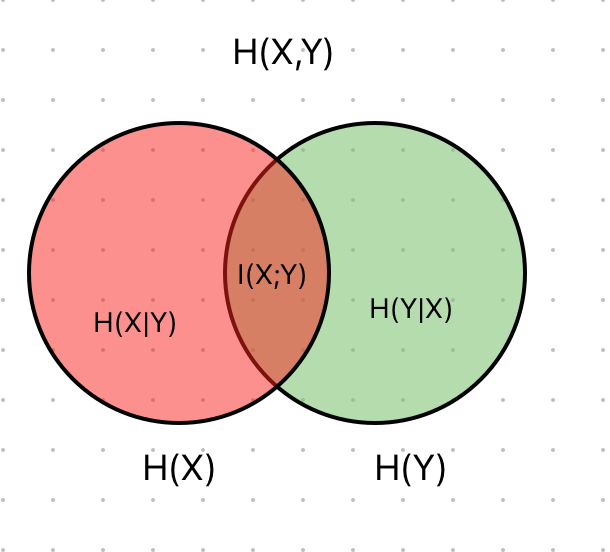
\includegraphics[width=0.6\textwidth]{Figs/Entropy_Venn.png}
    \caption{Relationship between entropy and mutual information}
    \label{fig:accumulator}
\end{figure}


\section{Capacity for Binary Input Memoryless Channels}
With entropy, joint entropy, relative entropy, conditional entropy, and mutual information defined, we are now to describe the important result of this chapter: channel capacity. Channel capacity defines the absolute upper limit for channel coding: in 1948, Shannon showed that no matter how clever we are, the channel codes have to operate below the channel capacity to achieve reliable communication. Equally astonishingly, Shannon showed that if the rate is below the channel capacity, then reliable communication is absolutely possible!

We will not give the full proof of this result in a general setting. Instead, we will give a short summary on the channel capacity of various binary input memoryless channels, describe the channel coding theorem, and prove one part of it.

\subsection{Channel Capacity}
\begin{definition}
    Channel Capacity: this is the maximal rate of reliable communication:
    \begin{align*}
        C = \sup{R| R \mbox{ is achievable}}
    \end{align*}
\end{definition}

\begin{theorem}
The channel capacity equals to the maximum mutual information.
\[C = \sup_{p_{X}(x)} I(X;Y).\]
where the supremum is taken over all possible choices of \(p_X(x)\).        
\end{theorem}

This is profound because it relates how much we can physically transmit over a channel reliably to the mutual information between input and output. This makes the complicated problem of finding channel capacity a clean optimization problem which involves finding the input distribution that maximizes the mutual information between the input and the output.

Let us state the Noisy-channel coding theorem in a formal way.
\paragraph{Noisy-channel coding theorem}
\begin{theorem}
The noisy-channel coding theorem states that for any error probability \(\epsilon > 0\) and for any transmission rate \(R\) less than the channel capacity \(C\), there is an encoding and decoding scheme transmitting data at rate R whose error probability is less than \(\epsilon\), for a sufficiently large block length. Also, for any rate greater than the channel capacity, the probability of error at the receiver goes to \(0.5\) as the block length goes to infinity.
\end{theorem}

\subsection{Noiseless Binary Channel}
Let us assume a channel whose binary input is reproduced exactly at the output. 

\begin{align*}
    C &= \max I(X;Y) \\
      &= \max H(Y) - H(Y|X) \\
      &= \max H(X) \\
      &= 1
\end{align*}
which is achieved by using \(p(x) = \{\frac{1}{2}, \frac{1}{2}\). 

\subsection{Binary Symmetric Channel}
The binary symmetric channel has symmetric crossover probability \(p\).

\begin{align*}
C = \max I(X;Y) \\
  &= \max H(Y) - H(Y|X) \\
  &= \max H(Y) - H(p) \\
  &\leq 1 - H(p)  
\end{align*}
this is achievable when \(p(x) = \{\frac{1}{2}, \frac{1}{2}\), when \(p(y=0) = p(y=1) = \frac{1}{2}\).
So the channel capacity of BSC is \(1-H(p).\) 

\subsection{Binary Erasure Channel}
In the binary erasure channel, a fraction \(p\) of the bits are erased and the received knows the location of the erasures. So the received bits can be \(01*0111\star01\cdot\), where \(star\) represents the erasures and the non-erasures are received correctly. 
\begin{figure}[h]
    \centering
    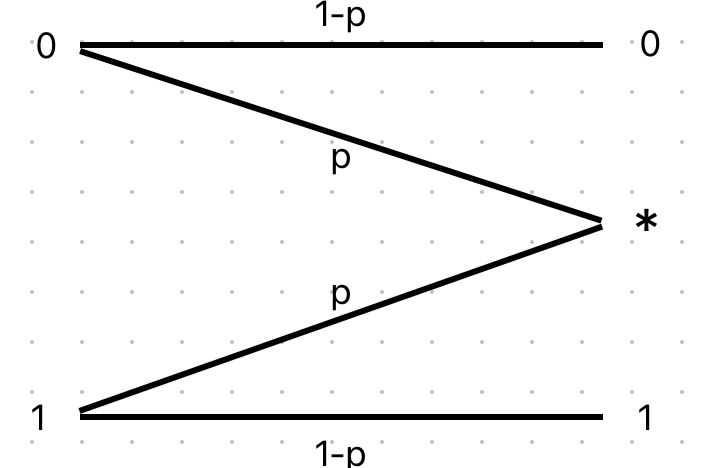
\includegraphics[width=0.5\textwidth]{Figs/BEC_channel.png}
    \caption{Binary Erasure channel. A bit has probability \(p\) erased; otherwise, it is received correctly. BEC is a good model for internet traffic.}
    \label{fig:accumulator}
\end{figure}

\begin{align*}
C = \max I(X;Y) \\
  &= \max H(Y) - H(Y|X) \\
  &= \max H(Y) - H(p) 
\end{align*}

Now assume \(p(x= 0) = \pi,\) then \(p(x=1) = 1- \pi\), and we have \(p(y=0) = \pi (1-p), \), \(p(y=1) = (1-\pi) (1-p), \) and \(p(y=\star)= p.\)
So 
\begin{align*}
    & H(Y) \\
    &= - \pi (1-p) \log (\pi (1-p)) - (1-\pi) (1-p) \log ((1-\pi) (1-p)) - p \log p \\
    &= (1-p)(-\pi \log (\pi) - (1-\pi)  \log (1-\pi)) - (1-p) \log (1-p)(\pi + (1-\pi))  - p \log p\\
         &= (1-p) H(\pi) + H(p). 
\end{align*}

Therefore \(C= \max H(Y) - H(p) = \max (1-p) H(\pi) = 1-p, \) where the maximum is achieved at \(\pi = \frac{1}{2}.\)

This being the upper limit for channel coding on the binary erasure channel makes intuitive sense: since the channel erases fraction \(p\) of the transmitted bits, the total redundancy we increase has to be at least \(p\) to have a change at reliable communication, otherwise what received is smaller than the intended information. So the code rate has to be less than \(1-p.\) 


\subsection{Binary input Additive White-Guassian-Noise Channel}
The Binary Additive White-Gaussian-Noise Channel (abbreviated as BAWGNC) is often used as a practical model in many digital communication schemes (such as transmission of data over a pair of wires). In practice, many types of noise sources are additive and independent of each other and thus, when added together, can be approximated by a zero-mean Gaussian random variable with some variance, say \(\sigma^2\). This approximation is justified by the central limit theorem.

The BAWGNC(\(\sigma)\) channel, as depicted in Figure 1, accepts a realization of a random variable \(X \in \{-1, +1\}\) on its input and outputs a realization of a random variable \(Y = X + Z\), where \(Z\) is a zero-mean Gaussian random variable with variance \(\sigma^2\). When combined together, we obtain the following conditional pdfs of Y
This channel is fully described by the noise variance \(\sigma^2\).

The capacity of this channel is given by the following formula

\[C_{BAWGN}(\sigma) = - \int_{-\inf}^{\inf} \Phi(y, \sigma) \log_2 \Phi(y, \sigma) dy - \frac{1}{2} \log_2 (2\pi \exp \sigma^2), \]

where \(\Phi(y, \sigma\) is a mixtured Guassian: 
\[\Phi(y, \sigma) = \frac{1}{2\sqrt{2\pi \sigma^2}} (\exp[-\frac{(y-1)^2}{2\sigma^2}] + \exp[-\frac{(y+1)^2}{2\sigma^2}]) \]

The derivation of this formula is beyond the scope of this class as it requires differential entropy. Interested students can find it in "Elements of Information Theory" by T. Cover and J. Thomas. 
\section{Channel Coding Theorem}
\begin{theorem}
For any error probability \(\epsilon > 0\) and for any transmission rate \(R\) less than the channel capacity \(C\), there is an encoding and decoding scheme transmitting data at rate R whose error probability is less than \(\epsilon\), for a sufficiently large block length. Also, for any rate greater than the channel capacity, the probability of error at the receiver goes to \(0.5\) as the block length goes to infinity.
\end{theorem}

\paragraph{Achievable Region}
Graphs for BSC, BEC, and AWGN will be included here. 

BSC: 1- H(p)
BEC: 1- p
AWGN: 

\subsection{A Sketch of the Proof of the Channel Capacity}
The channel capacity theorem states that if and only if the code rate is below the Shannon's limit, reliable channel coding scheme is feasible.  

At the heart of the proof is the typical set idea: given transmitted codeword \(c\), what received typically resides inside a shell of a sphere.

\subsubsection{Typical set}
Let us consider a transmitted codeword \(c\). The received message \(y\) will differ from \(c\) at \(pn\) positions with increasingly high probability; in fact, the probability that 
\[Pr(|d(y, c) - pn| > \epsilon) < \exp( - \epsilon^3 /n) \]
by Chernov's bound. That means for each transmitted codeword, the received vector is most likely with Hamming distance \(pn\) from the codeword, or we can say it resides in a shell around the codeword with radius \(pn\).  We call this is the typical set \(T_{p}(c)\) around codeword \(c\).

\subsubsection{If \(R > C\), then error probability is bounded away from \(0\)}
Here, we are going to prove one direction of the channel capacity theorem: if the code rate \(R\) is above the channel capacity, then it is impossible to achieve arbitrarily small error probability for at least some of the transmitted codewords. 

We actually can prove a stronger result. If the rate \(R\) is above the channel capacity, then the decoding error probability for some codeword has to be at least \(1/2\). 

The basic idea is: if the decoding error probability for a codeword is less than \(\frac{1}{2}\), then for the typical received vector, at least half of them should be in the decoding sphere around the codeword. So the volume of this sphere has to be large. That means we cannot pack too many such spheres, or too many codewords, into the linear space of \(2^n\). That gives the limit of the code rate.    



For reliable communication, these shells around codewords should be decoded correctly for at least half of them to achieve error rate less than \(\frac{1}{2}\).  


Let us first estimate the volume of each of these spheres. We need the Stirling's formula to approximate the factorials in the binomial expansion:  
\[n! = \sqrt{2\pi n} (\frac{n}{e})^n (1 + o(n)).\]

Since the sphere's volume is lower bounded by the half of the shell of distance \(pn\), we have
\begin{align*}
V_0 &\geq \frac{1}{2} \binom{n}{pn} \\
    &= p^{-pn}(1-p)^{-(1-p)n} (1 + o(n)) \\
    &= 2^{H(p)n - o(n)}
\end{align*}

This actually gives a physical interpretation of the entropy function: It represents the volume of the sphere around the codeword.  

Now consider totally how many codewords we can pack there with the constraint that these correct decoding regions do not overlap. This can be easily bounded: 
\begin{align*}
2^k V_0 &< 2^n \\
2^k 2^{H(p)n -o(n)} &< 2^n \\
k + H(p) n - o(n) &< n \\
R = k/n &< 1-H(p) - \epsilon 
\end{align*}
for any arbitrarily small $\epsilon$. In other words, if the code rate is above the Shannon's limit, then reliable communication is infeasible. 

\subsubsection{Typical Pairs Decoding}
Our decoding algorithm will be: if there is a unique codeword \(c\) within distance \((p + \delta)n\) from
the received word \(y\), decode to \(c\). Otherwise, give up. We will show that this works with high
probability.

\subsubsection{If \(R < C\), then error probability goes to \(0\) as \(n\) goes large}

If \(R < C\), then the total number of codewords is \(|C| = 2^{Rn} \leq 2^{(1-H(p)-\epsilon)n}.\)

What is the probability that our received word is not decoded properly? First, with probability
\(1− \epsilon\), the received word is close enough to the original codeword \(c\). In this case, the only reason
for the decoding to fail is if another codeword is also within \((p + \delta)n\) distance from the received
codeword. 

We will compute the probability that our received word is decoded to a specific other
codeword \(c^{'}\). Recall that the codewords were chosen at random. Thus, the probability that a
specific codeword \(c\) is within distance \((p + \delta)n\) from our received word \(y\) is exactly the probability
that a random binary string is within distance this of \(c^{'}\). This is just the ratio of the number of
words close to \(c^{'}\) to the total number of words, or approximately
\[\frac{2^{n H(p)}}{2^n} = 2^{-(1-H(p))n}.\]

Then by the union bound, the error probability that the typical pairs decoding makes an error is upper bounded by:
\begin{align*}
    P_{E} \leq |C| 2^{-(1-H(p))n} < 2^{-\epsilon n} 
\end{align*}
which goes to zero as \(n\) goes to infinity.
\newpage

%\Lecturer{Hui Jin}
\Contributor{}
\LectureNumber{05}
\LectureDate{DATE}
\LectureTitle{Cyclic Linear Codes}

\lstset{style=mystyle}

	\MakeScribeTop

%#############################################################
%#############################################################
%#############################################################
%#############################################################

\section{Introduction}
We have learned that for binary linear codes, the generator matrix, and equivalently the parity check matrix, determines the code structure. In particular, it determines the Hamming distance property of the code. 

But how we design the generator matrix so that we have codes either have good distance property, or can be efficiently encoded/decoded, or both? In this lecture, we discuss a simple way of constructing one type of generator matrices that have efficient implementation. The codes are known as cyclic linear codes. Cyclic linear codes rely on algebraic construction in design codes. 


Cyclic codes are instrumental to understand other algebraic codes, such as BCH codes, Hamming codes, and Golay codes. The algebraically sophisticated Reed Solomon codes are also cyclic codes, although non binary. 

In this lecture, we will cover the fundamentals of cyclic codes, its generator matrix, its parity check matrix, and its encoding and decoding algorithm. We also show how to use shift register circuits to implement encoder and decoders, which are extremely efficient.  

\section{Basic Properties of Cyclic Codes}
\begin{definition}
Cyclic codes are a subset of linear block codes that obey two essential properties: 
\begin{enumerate}
    \item The sum of two codewords is also a block  codeword; (the linear property); 
    \item Any cyclic permutation of the block codeword is also a block codeword. (the cyclic property)
\end{enumerate}
    
\end{definition}

So in addition to linearity, cyclic linear codes impose a cyclic shift symmetry: If bit-string \(c_0c_1, \cdots c_n\) is a codeword, then so is the left shift bit-string \(c_1c_2 \cdots c_nc_0\), and the right shift bit-string \(c_nc_0\cdots c_{n-1}\). Clearly, that means every \(i\) shift of the bit string is a codeword, for any integer value \(i\). 

In the following discussion, we focus on binary cyclic codes, even though the theory generalizes to q-ary cyclic codes. 

\section{Codeword Polynomial}
The fundamental tool to study cyclic linear codes is to associate a codeword with a polynomial. Assume the codeword is \(\c=(c_0, c_1, \cdots, c_{n-1})\), we associate it with the polynomial \(c(x)= c_0 + c_1 x + c_2 x^2 + \cdots + c_{n-1} x^{n-1}\). Henceforth, we will use the codeword and codeword polynomial interchangeably.  

Let us see what constraint the cyclic property imposes on this polynomial association. For the polynomial, the cyclic shift property translates to if \(c(x)\) is a codeword, then \(x^i c(x)\) is a codeword for any integer \(i\). That means \(xc(x) = c_0x + c_1 x^2 + c_2 x^3 + \cdots + c_{n-1} x^{n} \) should be equivalent to the polynomial corresponding to the codeword \(\c'=(c_{n-1}, c_0, \cdots, c_{n-2})\), which is \(c_{n-1} + c_{0}x + c_1 x^2 + c_2 x^3 + \cdots + c_{n-2} x^{n-1}\). So if we imposes that we limit polynomials mod \(x^n+1\), that indeed the cyclic property holds. 

\paragraph{generator polynomial}
Let us take a close look at the codeword polynomials. First there exists a generator polynomial.   

\begin{theorem}
Let \(\C\) be a binary \((n, k)\) linear cyclic code, and \(\C(x)\) the associated polynomials. There is \textbf{unique} monic polynomial \(g(x)\) in \(\C(x)\) with minimal degree \(r\).
\end{theorem}

\textbf{proof:} First since we focus on binary, all non-zero coefficients are \(1\), so all codeword polynomials are monic. As we have finite non-zero codeword polynomials, there must be some polynomials with minimal degree. If there are more than one such polynomials, we can assume \(\c_1(x), \c_2(x)\) are two of such polynomials, and their difference \(\c_1(x) - \c_2(x)\) is also a non-zero codeword but has smaller degree. Contradiction. 

This minimal degree polynomial \(\g(x)\) is the generator polynomial. 

\begin{theorem}
A polynomial \(\c(x)\) is a codeword if and only if it is a multiple of \(g(x)\).
\label{th:gx}
\end{theorem}


\textbf{Proof:} For any polynomial \(m(x)\), the product \(c(x) = m(x) g(x) = m_0 g(x) + m_1 xg(x) + \cdots m_k x^k g(x)\) must also be codeword because of linearity and cyclic property. 

Now given \(\c(x)\) is a codeword, let us divide \(\c(x)\) by \(\g(x)\) and write it as \(\c(x) = \m(x) g(x) + \d(x)\). If \(\d(x)\) is non-zero we have \(0 < degree(\d(x)) < degree(\g(x))\). However, in this case \(\d(x) = \c(x) - \m(x)\g(x) \) is also a codeword with smaller degree than \(\g(x)\) contradiction. So \(\d(x)\) must be zero, which means every \(\c(x)\) is a mulitple of \(\g(x)\). 

 In other words, for every codeword \(\c(x)\), there exists a \(\m(x)\), such that \(\c(x) = \m(x) \g(x)\), where the \(degree(m(x)) \leq k = n - r\).
 
\begin{theorem}
The generator polynomial \(g(x)\) is a factor of \(x^n +1\) in \(GF(2)(x)\).
\end{theorem}

\text{Proof:} Since \(x^n+1\) corresponds to the all zero codeword, by Theorem~\ref{th:gx}, \(x^n+1\) must be a multiple of \(\g(x)\). 

\section{Generator Polynomial Construction and Parity Polynomial}
We know any non-constant factor of \(x^{n} + 1\) can be a generator polynomial. If the degree of polynomial \(g(x)\) is \(r\), then every polynomial \(m(x)\) with degree \(n-r-1\) or less corresponds to a codeword \(c(x) = m(x) g(x)\). There are \(2^{n-r}\) such polynomials. Denote \(k=n-r\), a degree \(r\) generator polynomial \(g(x)\) produces a \((n,k)\) code. 

Given \(n\), what are the possible choices for such \(g(x)\)? If we factor \(x^n + 1\) into irreducible polynomials in \(GF(2)\), then the product any combination of these irreducible polynomials can be a \(g(x)\).

\begin{example}
We can factor \(x^7 + 1\) into the product of \((x+1)\), \((x^3+x^2+ 1)\), \((x^3 + x + 1),\) 
\[x^7 + 1 =(x+1)(x^3+x^2+ 1)(x^3 + x + 1), \]
therefore possible generator polynomial \(g(x)\) can be degree \(1\), degree \(3\) (there are two of them), degree \(4\) (there are two of them), or degree \(6)\). 
\end{example}

\begin{example}
The generator polynomial \(g(x)=(x+1)(x^3 + x^2 + 1)=x^4 + x^3 + x^2 + 1\) determines a \((7,3)\) cyclic linear code.  
Given a block of \(3\) bits, \(m=m_0m_1m_2m_3\), we first construct the message polynomial 
\[m(x) = m_0  + m_1 x + m_2 x^2 + m_3 x^3,\]
the codeword polynomial is 
\[c(x)=m(x) g(x).\]
\label{ex:cyclic74}
\end{example}

\subsection{Parity Polynomial}
\begin{definition}
The polynomial \(h(x)=(x^n+1)/g(x)\) is known as the parity polynomial. Given a codeword \(c(x)\), we see that \[c(x)h(x) = m(x) g(x) h(x) = 0 \pmod{x^n + 1}.\]
\end{definition}

\begin{example}
For \(g(x) = x^4 + x^3 + x^2 + 1\), the parity polynomial is \(h(x)=(x^7+1) / g(x) = x^3 + x^2 + 1\).
\end{example}


\section{Encoding of Cyclic Codes}
\subsection{Non-systematic encoding and Generator Matrix}
We have seen given the generator polynomial \(g(x)= g_0 + g_1 x + \cdots + g_{n-k} x^{n-k}\), we can encode a message polymial \(m(x) = m_0 + m_1 x + \cdots m_{k-1}x^{k-1}\) by polynomial multiplication \(c(x) = m(x) g(x)\), this is equivalent to 
\begin{align}
\c(x)  &= m(x) g(x) \nonumber\\ 
      &= m_0 + m_1 xg(x) + \cdots m_{k-1}x^{k-1}g(x) \\
      &= [m_0 \; m_1 \; \cdots \; m_{k-1} ]\begin{bmatrix}
           g(x) \\
           xg(x) \\
           \vdots \\
           x^{k-1} g(x)
         \end{bmatrix} \nonumber
\end{align}

If we focus on just the coefficients of \(c(x)\), we get the following generator matrix form: 
\begin{align}
    \c &= [m_0 \; m_1 \; \cdots \; m_{k-1} ] \nonumber
    \left(
    \begin{array}{cccccccc}
      g_0 & g_1 & \cdots & g_{r} & & & & \text{\huge 0} \\    
          & g_0 & g_1    & \cdots & g_r& & & \\
      &   &     & \ddots & \ddots & \ddots & &         \\
        & &      & g_0 & g_1 & \cdots & g_{r} &        \\
     \text{\huge 0} & &      &    & g_0 & g_1 &\cdots & g_{r}          
    \end{array}
    \right) \\
       &= \m \G \nonumber 
\end{align}

\begin{example}
    In example\ref{ex:cyclic74}, our generator polynomial is \(g(x) = x^4 + x^3 + x^2 + 1\), so the generator matrix of the \((7,3)\) code defined is 
    \begin{align*}
   G=\left[
   \begin{array}{ccccccc}
      1 & 0 & 1 & 1 & 1 & 0 & 0 \\
      0 & 1 & 0 & 1 & 1 & 1 & 0 \\
      0 & 0 & 1 & 0 & 1 & 1 & 1 \\
      \end{array}
   \right]
\end{align*}
\end{example}


\subsection{Parity Check Matrix of Cyclic Codes}
Just like the generator matrix, it is straightforward to find a parity check matrix of cyclic codes give the parity check polynomial \(h(x)\). Note that \(degree(h(x)) = k\) and we assume \(h(x)) = h_0 + h_1 x + h_2 x^2 + \cdots + h_k x^k.\)

We know that \(c(x)h(x) = m(x)g(x)h(x) = 0 \pmod{x^n+1}.\) Therefore, 
\begin{align}
\textbf{0}  &= c(x) h(x) \nonumber\\ 
      &= c_0 + c_1 xh(x) + \cdots c_{n-1}x^{n-1}h(x) \\
      &= [c_0 \; c_1 \; \cdots \; c_{n-1} ]\begin{bmatrix}
           h(x) \\
           xh(x) \\
           \vdots \\
           x^{n-1} h(x)
         \end{bmatrix} 
         \nonumber
\end{align}
Note that the operation above are all \(\pmod{x^n+1}\). Every coefficient  of the above polynomial \(c(x)h(x)\) is \(0\), which gives \(n\) constraint. If we write in the matrix form, we have 

\begin{align}
    \textbf{0} &= [c_0 \; c_1 \; \cdots \; c_{n-1} ]  
    \left(
    \begin{array}{cccccccc}
      h_0 & h_1 & \cdots &  & h_{k} & & & \text{\huge 0}&  \\    
          & h_0 & h_1    & \cdots & & h_k& & & \\
      &   &     & \ddots & \ddots & & \ddots & &           \\
             & &      & & h_0 & h_1 & \cdots & h_{k}        \\
        h_{k}  &    &     &  &   & h_0 &\cdots& h_{k-1}      \\
        h_{k-1}&h_k &     &  &   &     & h_0 &\cdots          \\
        \vdots &   &      &  &   &     &     & \vdots          \\
        h_{1} & h_2 &\cdots&h_k& &    &      & h_0         \\
    \end{array}
    \right) 
\end{align}

Even though there are \(n+1\) parity checks, we know only \(n-k\) of them are linearly independent, as the rank of the parity check matrix is \(n-k\). We pick the last \(n-k)\) parity checks, and that gives us 

\begin{align}
    \textbf{0} &= [c_0 \; c_1 \; \cdots \; c_{n-1} ]
    \left(
    \begin{array}{ccccc}
          h_{k}  &      &       & & \text{\huge 0} \\    
          h_{k-1}& h_k  &       &       &  \\
         h_{k-2}&h_{k-1}& h_{k} &       &  \\
          \vdots&\vdots & \vdots&       &   \\
           h_{0}& h_{1} & \cdots& h_{k}    &   \\
                & h_{0} & h_{1} & \cdots   &  h_{k}    \\
                &        & \ddots& \ddots   & \ddots           \\
        \text{\huge 0} & &       &          & h_0      \\
    \end{array}
    \right) \label{eq:Hmatrix}
\end{align}
Contrast this with the generator matrix and notice the similarity and difference. 

\begin{example}
    In example\ref{ex:cyclic74}, our parity polynomial is \(h(x) = x^3 + x^2 + 1\), so the parity check matrix of the \((7,3)\) code defined is 
    \begin{align*}
   H=\left[
   \begin{array}{ccccccc}
      1 & 1 & 0 & 1 & 0 & 0 & 0 \\
      0 & 1 & 1 & 0 & 1 & 0 & 0 \\
      0 & 0 & 1 & 1 & 0 & 1 & 0 \\
      0 & 0 & 0 & 1 & 1 & 0 & 1 \\
      \end{array}
   \right]
\end{align*}
\end{example}
Note that parity check matrix is defined as the transpose of the matrix in Eq.~\ref{eq:Hmatrix}.

\paragraph{class break}

\section{Systematic Encoding}
In practice, it is advantageous to have systematic encoding where message bits are part of the codeword, often appended in the front or the back part of the codeword bits. We can easily modify the encoding algorithm of the cyclic codes to make it systematic, with the generator polynomial \(g(x)\).

The message polynomial is \(m(x) = m_0 + m_1 x + \cdots m_{k-1}x^{k-1}\), we claim the following: 
\begin{theorem}
Let \(d(x)\) be the remainder of \(x^{r} m(x)\) divided by \(g(x)\). Then \(x^{r} m(x) - d(x)\) is a codeword; and the codeword associated is \(d_0, d_1, \ldots, d_{r-1}, m_0, \ldots, m_{k-1})\).
\end{theorem}

\paragraph{proof:} To show a polynomial is a codeword with generator polynomial \(g(x)\), we need to show that the polynomial is a multiple of \(g(x)\). Now by definition, \(d(x) =x^{r} m(x) \pmod{g(x)}\), which means \(x^{r} m(x) - d(x) = 0 \pmod{g(x)}\). Therefore, \(x^{r} m(x) - d(x)\) is a codeword. Note that \(d(x)\) is a remainder so its degree is less than the degree of \(g(x)\), which is \(r\), therefore the coefficients corresponding to \(x^{r} m(x)\) and that corresponding to \(d(x)\) do not co-mingle. Thus the codeword associated with \(x^{r} m(x) - d(x)\) is \(d_0, d_1, \ldots, d_{r-1}, m_0, \ldots, m_{k-1})\), which is systematic.  

\begin{example}
    Systematic encoding of the \((7,4)\) code defined Example~\ref{ex:cyclic74}. Consider the encoding of the message block \(101\). 

    \begin{itemize}
        \item Compute \(x^{n-k} m(x) = x^4 (x^2 + 1) = x^6 + x^4\)
        \item Compute the remainder \(x^6 + x^4\) divided by \(x^4 + x^3 + x^2 + 1\). We use long division to get \(d(x) = x + 1\).
        \item The codeword is \(x^4m(x) + d(x) = 1 + x + x^4 + x^6\), which corresponds to \(1100101\).
    \end{itemize}

    We can show the following encoder table. 
\end{example}


\section{The shift register view of encoding}
We can implement the encoding of cyclic linear codes on a shift-register circuit, operation of which can be extremely efficient. 

First let us consider non-systematic encoding, which is represented by \(c(x) = m(x) g(x)\). Figure~\ref{fig:CyclicEncoder} shows the shift register circuit. The circuit has a master clock, where values on the circuit are updated as the clock ticks. In the figure, a symbol \fbox{D} represents a register, which latches the input value as clock ticks. A symbol \circled{g} represents a multiplication by number \(g\); since we are in binary field, \(g=1\) means there is a wire and  \(g=0\) means there is no wire. A symbol \circled{+} represents the XOR (mod 2 sum) operation. 

Message bits \(m_{k-1}, m_{k-2}, \ldots, m_0\) are fed into the circuit in the first \(k\) clocks, one bit each clock, in that order. The next \(n-k\) clocks takes no further inputs but circuit keeps updating its values. After \(n\) clocks, the circuit finishes computing the polynomial multiplication \(c(x) = m(x)g(x)\) and the registers have the values \(c_0, c_1, \cdots, c_{n-1}.\)  

\begin{figure}[ht]
    \centering
    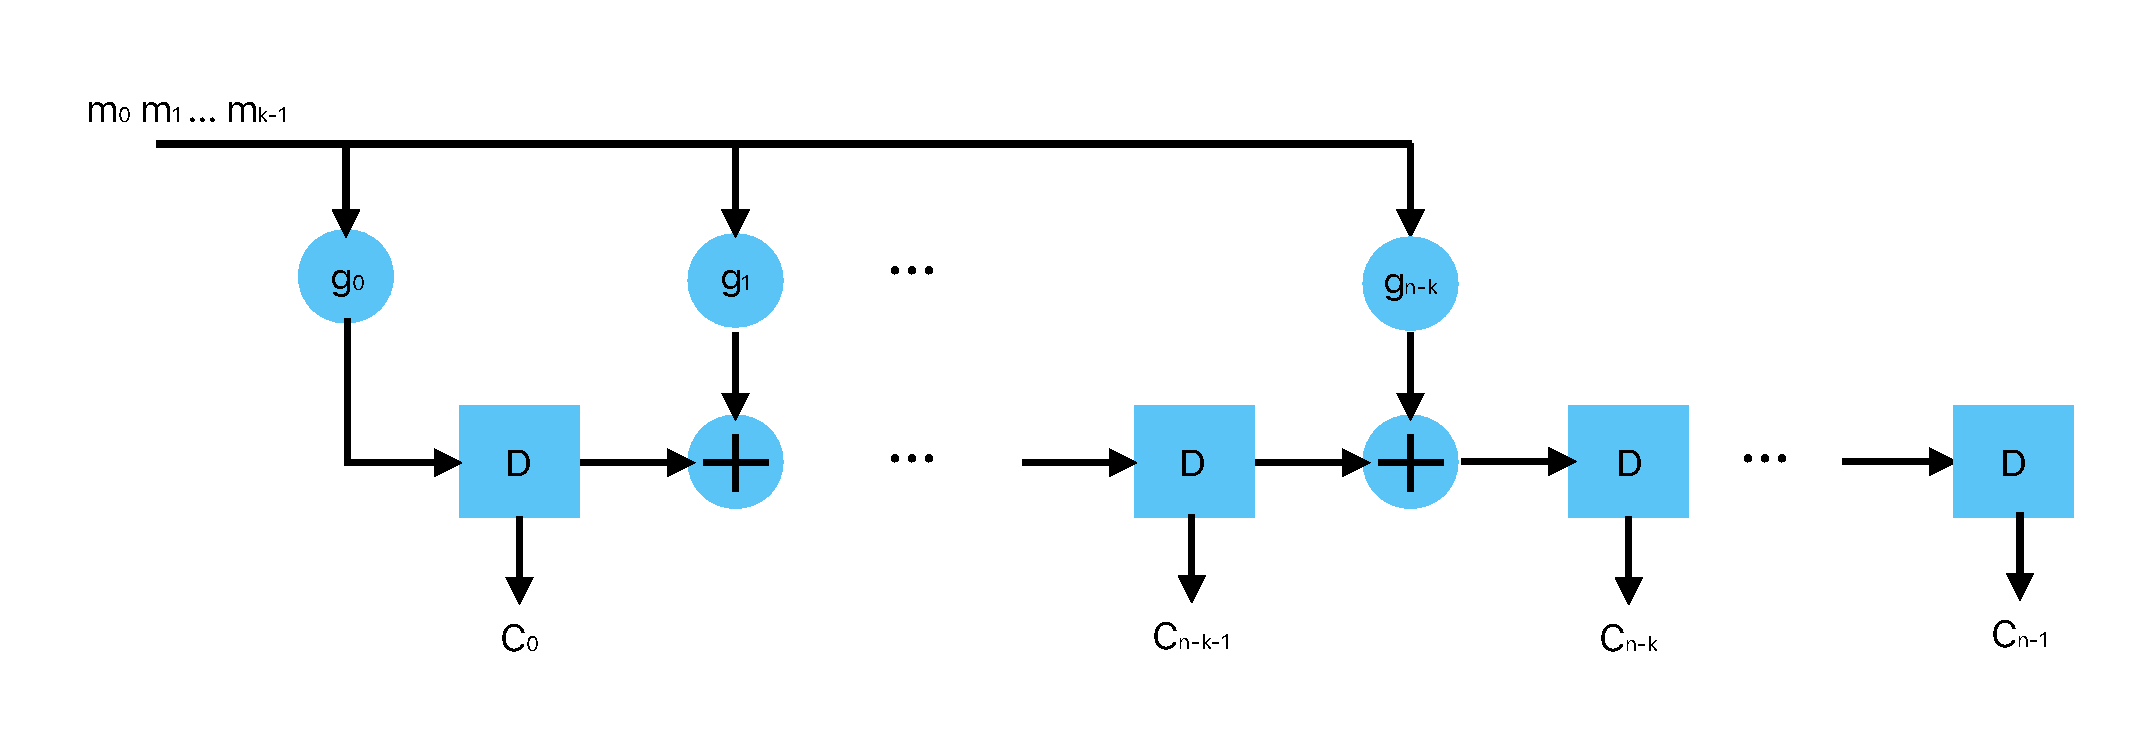
\includegraphics[width=1.0\textwidth]{Figs/CyclicCodesEncoder.pdf}
    \caption{General shift register circuit for a non-systematic encoder}
    \label{fig:CyclicEncoder}
\end{figure}

\begin{example}
Let us consider the encoding circuit for the \((7,3)\) code defined by the generator polynomial \(g(x)= x^4 + x^3 + x^2 + 1\) as in Example~\ref{ex:cyclic74}.
\begin{figure}[ht]
    \centering
    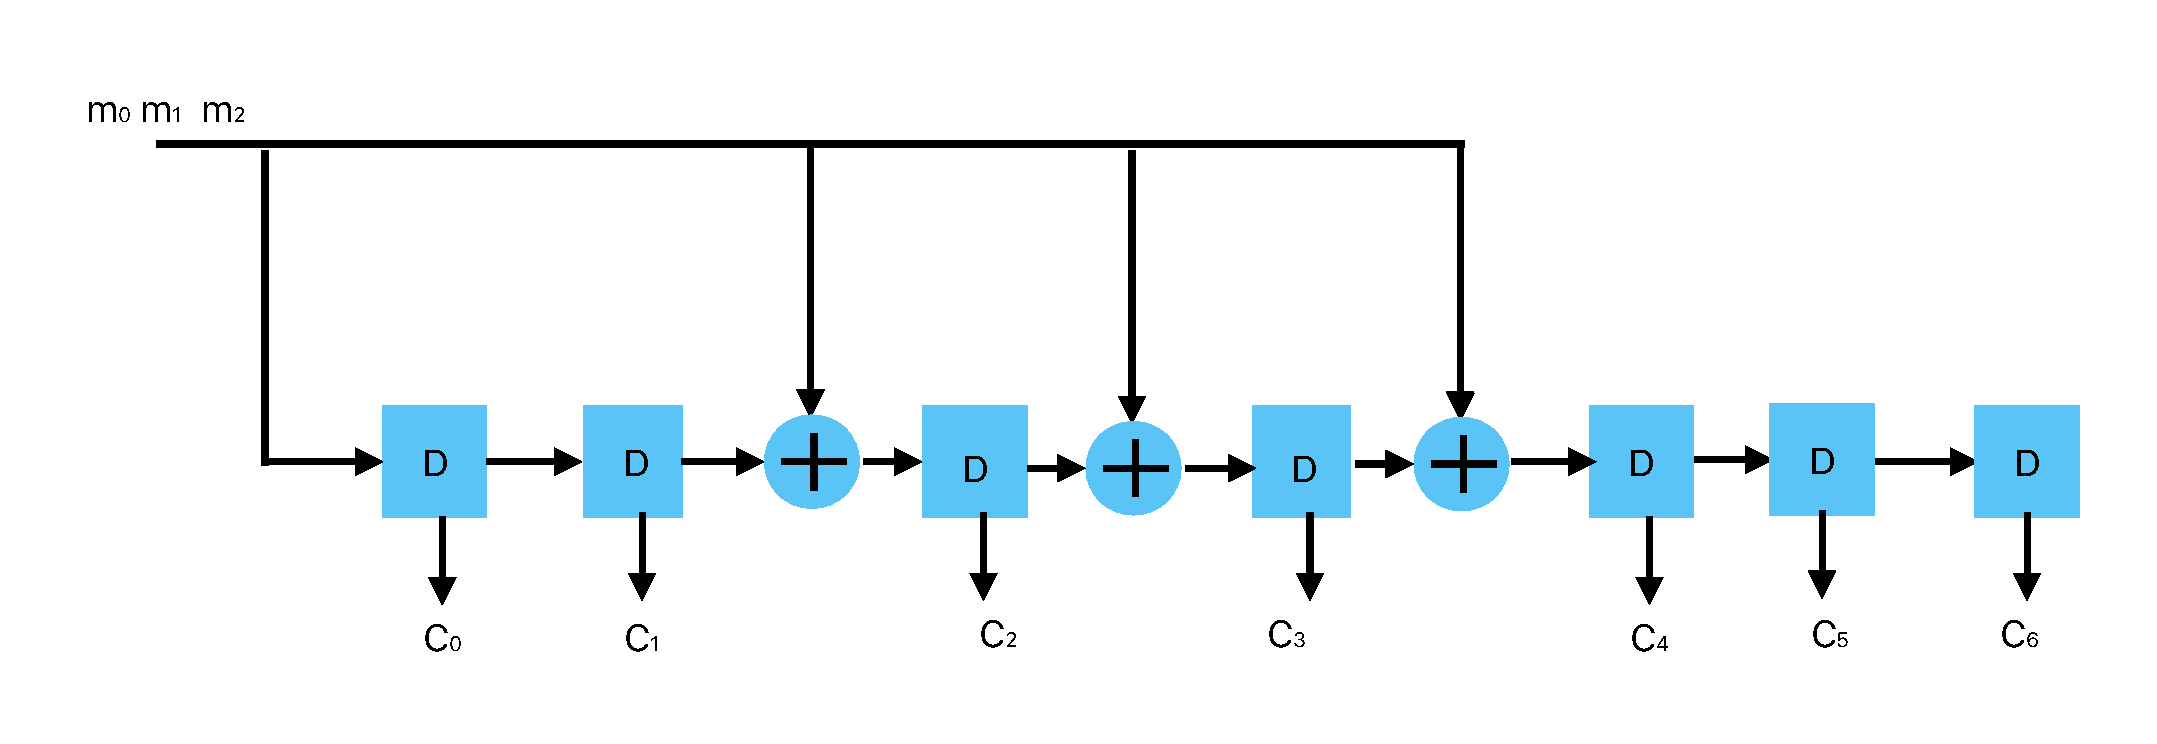
\includegraphics[width=1.0\textwidth]{Figs/SR_encoder73.pdf}
    \caption{(7,3) Encoder for the code defined in Example~\ref{ex:cyclic74} }
    \label{fig:CyclicEncoder}
\end{figure}

\end{example}


\subsection{Shift register circuit for systematic encoder}
The systematic encoding requires slightly more complicated circuit. It uses the linear-feedback shift register (LFSR) structure. The circuit computes the \(d(x) = x^{n-k} m(x) \pmod{g(x)}\). Here we will use the Example~\ref{ex:cyclic74}  to show the encoding circuits and steps. 

\begin{example}
Let us consider the systematic encoding circuit for the \((7,3)\) code defined by the generator polynomial \(g(x)= x^4 + x^3 + x^2 + 1\) as in Example~\ref{ex:cyclic74}. It has two parts: 
\begin{enumerate}
    \item The circuit for \(x^4 m(x) = x^6 + x^4 \) can be simply done by appending four zeros at the end of the input bits. We have \(m=(101)\), so the new input is \(0000101)\).   
\item Figure~\ref{fig:CyclicEncoderSystematic} shows the circuit for polynomial division of any polynomial \(p(x)\) by generator polynomial \(g(x)\). 
\end{enumerate}

\begin{figure}[ht]
    \centering
    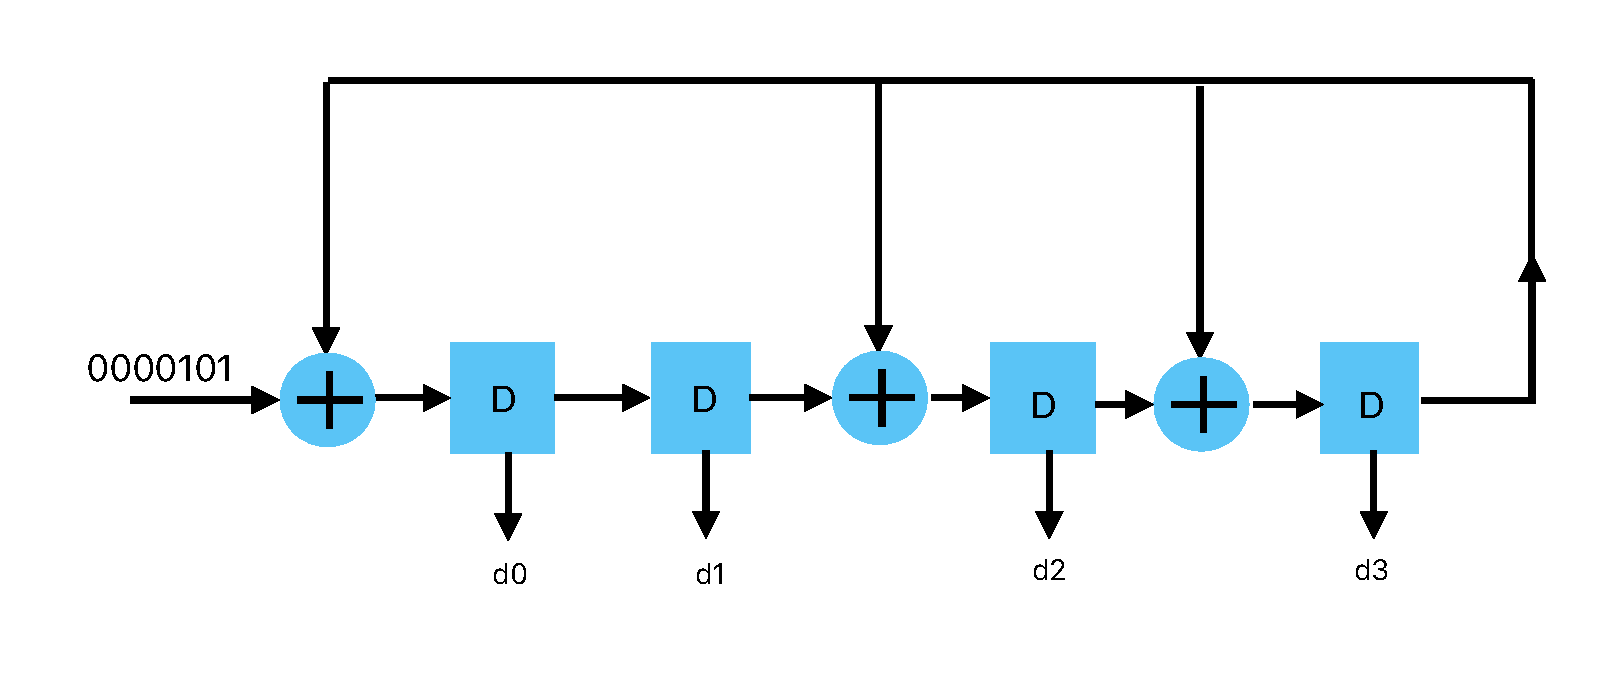
\includegraphics[width=1.0\textwidth]{Figs/SR_systematic_73.pdf}
    \caption{(7,3) Encoder for the code defined in Example~\ref{ex:cyclic74} }
    \label{fig:CyclicEncoderSystematic}
\end{figure}

The idea of the circuit is very simple; it corresponds directly to polynomial long division. The \(d(x)\) holds the current degree \(4\) polynomial as in the long division. If the leading coefficient \(d_3\) is \(1\), we subtract \(g(x)\) from the \(d(x)\); and the next \(d'(x) = x d(x)\).   

\end{example}


\section{Detection and Decoding}
Consider systematic encoding with generator polynomial \(g(x)\), we generate codeword \(c(x) = c(x)=x^{n-k}m(x) + d(x)\), where \(d(x) = x^{n-k}m(x) \pmod{g(x)} \). We will show that error detection is extremely easy and efficient, and error correction can apply syndrome decoding with a smaller look-up table. 

\subsection{Detection}
Given a received vector \(r(x)\) with systematic encoder, we can check whether it is a multiple of \(g(x)\) to detect error. A correct codeword is \(x^{n-k}m(x) + d(x)\). Assuming the input is \(m(x)\), we can use the exact encoding circuit to generate \(d(x)\). If \(r = [d', m]\) and \(d'(x) \neq d(x)\), then an error is detected.

\subsection{Decoding}
The difference \(s(x) = d'(x) - d(x) = (x^{n-k}m(x) + d'(x)) - (x^{n-k}m(x) + d(x)) = r(x) - c(x)\) is the syndrome of the received vector. Thus the syndrome \(s(x) = r(x) \pmod{g(x)}\).

\newpage

%\Lecturer{Hui Jin}
\Contributor{}
\LectureNumber{06}
\LectureDate{DATE}
\LectureTitle{Convolution Codes}

\lstset{style=mystyle}

	\MakeScribeTop

%#############################################################
%#############################################################
%#############################################################
%#############################################################

\section{Introduction}

Voyager 1, which was launched in 1977, has left the solar system. It has been transmitting scientific data back to earch until December 2023.  The 20W transmitter on the Voyager 1 had to cover tens of billions of kilometers for this transmission, thus the best known codes at the time was deployed. The codes used are convolutional codes, and the decodign algorithm used is known as Viterbi decoding. 

Later, convolutional codes were again used in the Cassini probe, this time the destiny was Saturn, launched in 1997.  Two convolutional codes, rate one-half and rate one-sixth, are used. To achieve low bit error rate, the convolutional codes are used as an inner code and concatenated with a Reed-Solomon outer code. 
The convolutional codes achieve a bit error rate (BER) of 0.5\%.  And then the outer Reed-Solomon corrects this small error rate. The overall BER of this concatenated code is below \(10^{-6}\).

In this lecture, we will explain Convolutional codes, and the three different views on convolutional codes: the shift-register view, the state space view and the trellis view. These different views are all useful in understanding convolutional codes. 

In next lecture, we will cover how to decdode convolutional codes.

\section{An Example Convolutional Code}
Many block codes used the idea of parity bits, where bits are inserted to create parity checks. Convolutional codes also insert parity bits. But instead of to fixed block of information bits, it insert parity bits to a stream of bits. 


We describe convolutional codes by giving the
equations for the parity bits.  Here is a simple convolutional code. (Even though this is a simple example, it captures all essential elements of any convolutional codes and we will use it to illustrate all important ideas.)
Assume information bits are \(x_1, x_2, \ldots\), we are going to generate parity bits in a streaming way: At time \(n \geq 0\), 
\begin{align*}
p_0[n] &= x[n] + x[n-1] + x[n-2] \\
p_1[n] &= x[n] + x[n-2],    
\end{align*}
here we assume \(x[-1], x[-2]\) are initialized as \(0\). So there are two streams of parity bits generated. 

Let us see how we encode the following message: \(101011\). We assume the right most bit comes first, or the beginning of the stream, to be consistent with the convention we used in cyclic codes. So we have \(x[0] = 1, x[1] = 1, x[2] = 0, \) etc.  This is how we are thinking of the message as a stream.

We further assume \(x[-1] = x[-2] = 0\) so that the equations above make sense at the initial state. At time \(n=0\), \(x[0]x[-1]x[-2] = 001\).  

So we have \(p_0[0] = 1 + 0 + 0 = 1\), and \(p_1[0] = 1 + 0 = 1\).

At \(n=1\), the used message bits are \(x[1]x[0]x[-1]=110\) and our parity bits generated are \(p_0[1] = 1 + 1 + 0 = 0\) and \(p_1[1] = 1 + 0 = 1\).

At \(n=2\), the used message bits are \(x[2]x[1]x[0]=011\) and our parity bits generated are 

\(p_0[2] = 0 + 1 + 1 = 0\) and \(p_1[2] = 0 + 1 = 1\).

For transmitting, we usually send the parity sequences, excluding the message.  When we have multiple parity equations, we interleave the bits of the parity sequences.  Therefore, the codeword is the interleaved version of the parity bits \( \cdots, p_0[2], p_1[2], p_0[1], p_1[1], p_0[0], p_1[0]\). For this example code, a running \(k\) information bits will generate \(2k\) coded bits, the code rate of this convolutional codes is \(\frac{1}{2}.\) (Later we will see there is a minor correction to that.)


So we are generating the parity bits by using a slide window over the message bits. The width of this window (in bits) is called the code's constraint. We denote \(K\) as the constraint. In this example, \(K=3.\)


In the above example, each message bit is "spread across" \(K\) elements of each parity
sequence, so the parity sequences are better protection against bit errors than the message sequence itself.

This is the property of a non-recursive convolutional code. 


\section{Difference Between Convolutional Codes And Block Codes}
The most obvious differences between convolutional codes and linear
block codes are:
\begin{enumerate}
    \item Convolutional codes act on message bits streaming into the encoder. 
    \item Parity bits are generated over a sliding window of message bits, ie it is localized.
    \item We transmit \textbf{only} parity bits, excluding data bits.
\end{enumerate}
   
This means that convolutional codes are non-systematic codes.

The way we will be able to get error correction properties out of convolutional codes is by having each message bit affect many different parity bits (in some sense: a particular message bit will be involved in many different parity equations).

The code rate of these types of codes tells us how many parity bits are sent for each message bit.  We will be talking mostly about \(1/r\) codes (i.e., \(r\) parity bits per message bit). 

Although the code rate seems fixed for the convolution code structure, we can achieve different rates by puncturing. We will talk about that later. 

\section{Representing Convolution Codes}
There are a lot of different ways to visualize/describe convolutional codes. Mastering all these different views is essential to understand convolutional codes. 

\subsection{Shift-Register view}
  The first is the "shift-register" view, which actually
reflects how this coding process might be implemented in hardware.

For the example we have above, here is the shift-register view:

\begin{figure}[h]
    \centering
    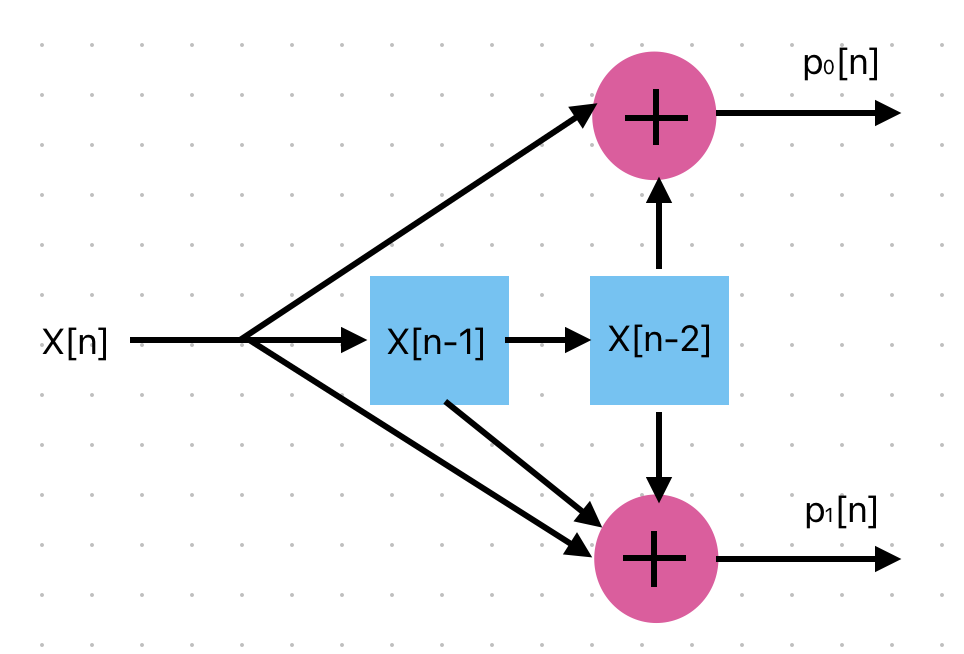
\includegraphics[width=0.6\textwidth]{Figs/Conv_Register.png}
    \caption{Caption}
    \label{fig:Conv_Register}
\end{figure}
Here \(x[n-1]\) and \(x[n-2]\) are held in two registers.  A new bit, \(x[n]\), arrives
at the left.  The box computes the parity bits from the incoming bit
\(x[n]\) and the \(2\) previous message bits.  At the end of the iteration,
the saved message bits are shifted right by one, and the incoming bit
moves into the left position.

A simpler way to represent the shift register view is to directly use the register elements, denoted by \(D\). 

\begin{figure}[h]
    \centering
    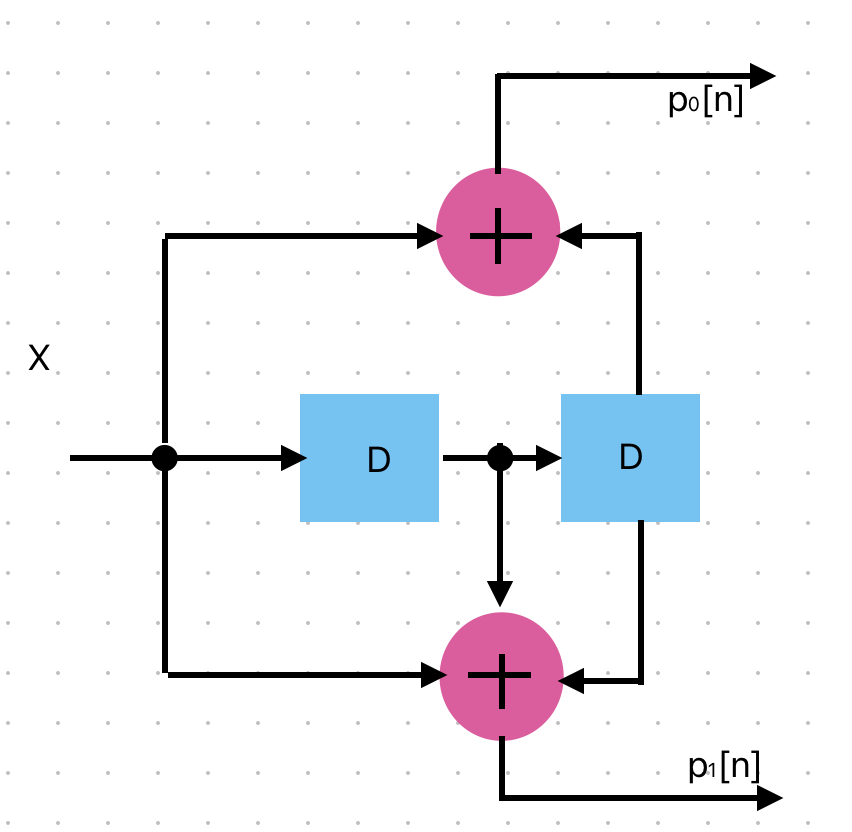
\includegraphics[width=0.6\textwidth]{Figs/Conv_FIR.png}
    \caption{Caption}
    \label{fig:Conv_Register}
\end{figure}


At the start of encoding, we assume \(x[-1]\) and \(x[-2]\) contain zero. When we finish, we add \(K-1\) zeroes to the end of the code, to allow the
registers to "settle", again at zero. For long block length, these resetting bits do not materially affect the code rate. 

\subsection{Generator Polynomial or Transfer Function}

Just like block codes, where a generator matrix is useful to describe a code, we also have generator nottaion to succinctly represent convolutional codes. In fact, we have a set of generators, where generator \(g_i\) is the generator for parity bit \(p_i\).

The generator basically shows which register contributes to the parity bit. For example, for parity stream \(p_0 = x[n] + x[n-1] + x[n-2]\), the generator polynomial \(g_0(D) = 1 + D + D^2\), or more simply \(g_0 = [111]\). For parity stream \(p_1 = x[n] + x[n-2]\), the generator is polynomial is \(g_1(D) = 1+ D^2\), or \([101]\). 

\paragraph{Transfer Function}
If we apply a z-transform to the equation \(p_0 = x[n] + x[n-1] + x[n-2]\), we have 
\[P = X(1+ D + D^2),\] so 
\[G(D) = \frac{P}{X} = 1 + D + D^2.\] 
This is know as the transfer function for the first parity bit of the convolutional code.  

The generator polynomial  relates directly to our shift-register view, as shown in  the diagram. 


With these generators, we can express the parity bits in a different way.  A convolutional code generates sequences of parity bits from
sequences of message bits by a convolution operation:

   \[p_i[n] = \sum_{j=0}^{K-1} g_i[j] x[n-j] = g \circledast x\]
where \(g_i[j]\) is the coefficient of term $D^j$,  
$K$ is, again, the constraint length. Again, \(g_i(D)\) is the K-element generator polynomial for parity bit \(p_i\).

The convolutional nature of parity bits generation leads to the name convolutional code. 

Regarding the constraint length K, the larger K is,
the more times a particular message bit is used when calculating parity bits.  This will lead to greater redundancy, and usually to better error correcting possibilities.



\section{State Space View}
In this section we briefly review the state-space approach to convolutional codes.

An \((n, k, m)\) convolutional encoder is a linear sequential device which maps a sequence of $k$-dimensional information, of input blocks \(x_1, x_2, \cdots\), over the finite field \(GF(2)\),  into a sequence of $n$-dimensional output, of output blocks \(p_1, p_2, \cdots\)

The encoder also passes through a sequence of internal $m$-dimensional state vectors, or simply states \(s_0 , s_1, \cdots\). The $j$th code block \(c_j\) is a linear function of the $j$th input block \(x_j\) and also of the $j$th state \(s_j\). This is precisely a linear system, defined over the finite field \(GF(2)\).


The formal description of the encoder’s operation is  this: the initial state \(s_0\) is assumed to be the zero state and for \(j \geq 0\), the linear system evolves as:
\begin{align}
 s_{j+1} &= s_j A + x_j B  \label{eq:state} \\
 p_j &= s_j C + x_j D \label{eq:output}
\end{align}
where the four matrices \(A, B, C,\) and \(D\) have entries from GF(2) and dimensions \(A:m \times m; B:k \times m; C:m \times n; D : k \times n\).

For the code defined in the example,  the linear system is:  
\begin{align*}
s_{j+1} &= s_j \begin{bmatrix}
    1 & 0 \\
    0 & 0
\end{bmatrix} + x_j  \begin{bmatrix}
    0 & 1 \\
\end{bmatrix} \\
p_{j} &= s_j \begin{bmatrix}
    1 & 1 \\
    1 & 0
\end{bmatrix} + x_j  \begin{bmatrix}
    1 & 1 \\
\end{bmatrix} 
\end{align*}

The \((n,k,m)\) convolutional code associated with such an encoder is then defined to be the set of all possible output sequences (or codewords) \(p_0, p_1, p_2, \cdots\) which can be produced form the encoder, starting with the initial state \(s_0 = 0\).

Let us represent the example convolutional code using the state space view. 

\begin{center}
\begin{tabular}{|c|c|c|c|}
\hline
\(x_n\) & \(s_n[0]s_n[1]\) & \(p_n[0]\) & \(p_n[1]\) \\ \hline
1 & 10 & 1 & 1 \\ 
1 & 11 & 0 & 1\\
0 & 01 & 0 & 1\\
1 & 10 & 0 & 0\\ 
0 & 01 & 1 & 0\\
0 & 00 & 1 & 0\\
\hline
\end{tabular}
\end{center}

The state transition can be represented by a state machine graph, where transitions are shown by arrows pointing from the current state to the next state. On each transition, we associate the bits \(x/p_0p_1\) where \(x\) is the input bit and \(p_0p_1\) are the two parity bits.  

\begin{figure}[h]
    \centering
    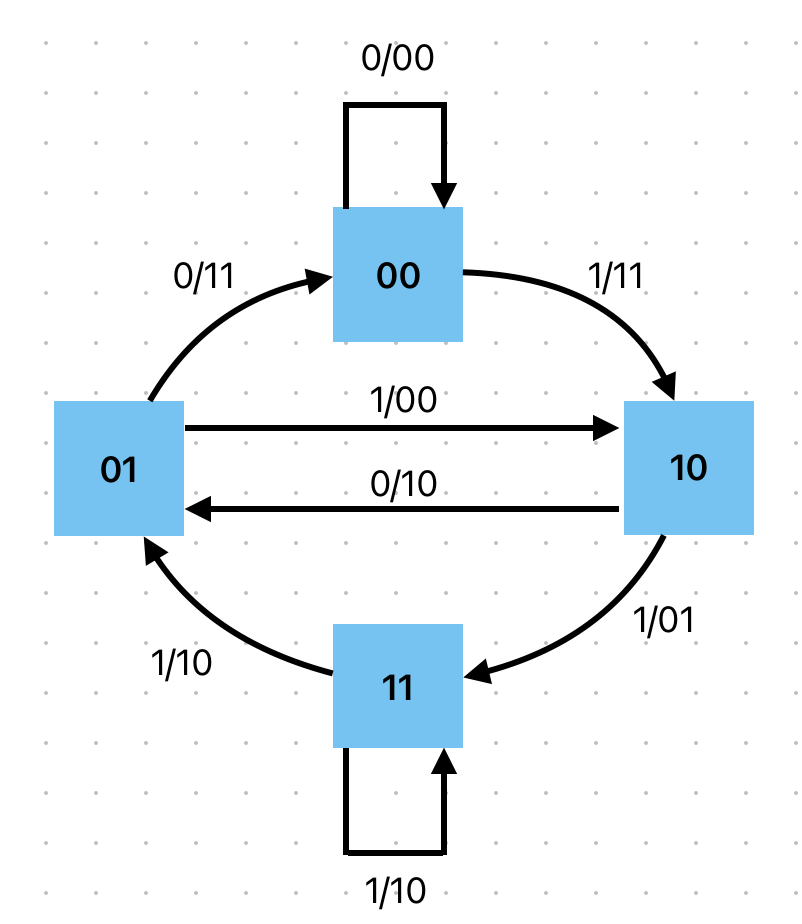
\includegraphics[width=0.6\textwidth]{Figs/ConvStateSpace.png}
    \caption{State Machine View of the Example Convolutional Codes}\label{fig:ConvStateSpace}
\end{figure}

\paragraph{Break here}

\section{Trellis View}
The state machine alone is pretty useful.  But it only gives a visual
representation of where we are at iteration n.  It would be nice to
have a representation that kept track of what states we had been in
previously.

(In fact, when we learn how to decode convolutional codes, it's going
to be \textbf{very} nice)

What we will do is, essentially, take the state machine and spread (unroll) it out over time.  This is called the "trellis" view.  With this view, we can trace a path over time; each path corresponds to a valid codeword. 

In the trellis view, we will only label the transitions with the
parity bits, instead of always including \(x[n]\).  We do this because of
the two arrows exiting a transition, the upper arrow always
corresponds to \(x[n]=1\), and the lower arrow always corresponds to
\(x[n]=0\).

Figure~\ref{fig:ConvTrellis} shows the trellis structure for our example convolutional codes. 
\begin{figure}[h]
    \centering
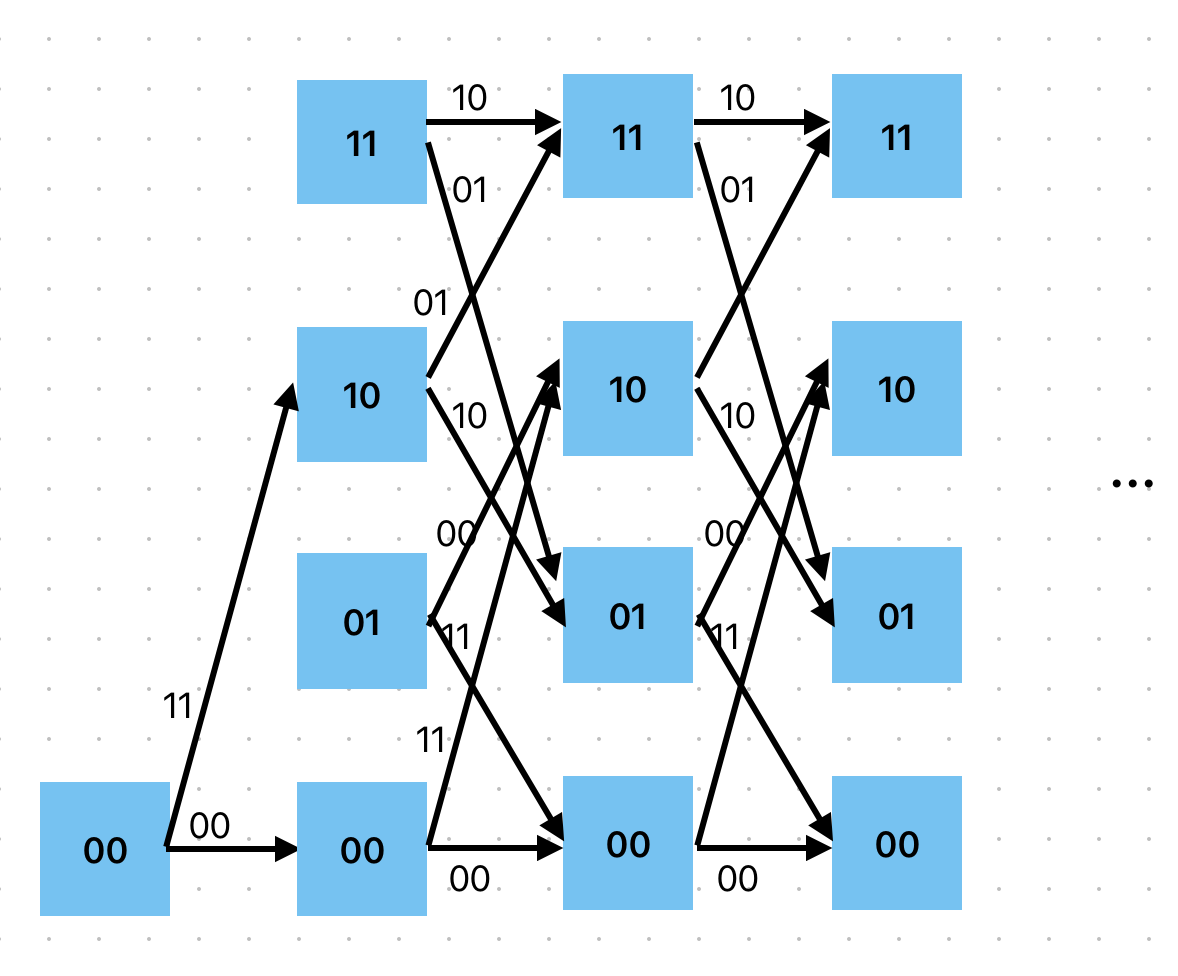
\includegraphics[width=0.6\textwidth]{Figs/ConvTrellis.png}
    \caption{State Machine View of the Example Convolutional Codes}\label{fig:ConvTrellis}
\end{figure}


Our encoding procedure now can be described straightforward:  Beginning at the starting state,
for each message bit, make the appropriate state transition, and send \(p_0p_1\).  Then end the message with \(K-1\) zeros, to ensure return to the
starting state.

Any path through the trellis corresponds to a code word.  We could
also consider the subset of paths that start in the zero state and end
at time step \(N\) in the zero state these would generate codewords of
length N. The original message bits can be read off by noting
whether the path at each stage takes the upper branch (bit \(0\)) or lower
branch (bit \(1\)). And the codeword bits can be read off from the labels
on the traversed path.

Let us show how we encode the example message bits \(
101011\). This should be a path along the states from six steps. In reality, we might need to terminate the message bits using \(00\) so that the state returns to the all zero state. 

This termination loses a bit information bit, but is not important. 

Because the states are binary strings, we can  interpret them as decimal numbers, 
  "00, 01, 10, 11" as \(0,1, 2, 3\). Such representation is useful in implementation.

\section{Free Distance of Convolution Codes}

The parity stream forms a linear code (the parity bits are linear functions of the data bits).

The fact that parity bits are linear functions of the data bits is essentially saying that \(c=Gx\), which establishes the linearity of the code.

 In view of the convolution expression for the parity bits, it follows that the sum of two
  parity streams is a parity stream (the stream corresponding to the sum of the two data words).

The smallest-weight nonzero codeword has a weight that, locally in time, plays a role analogous to \(d\) (the minimum Hamming distance). It's called the free distance of the convolutional code; we'll denote
it \(d_{free}\).

Specifically, the free distance \(d_{free}\) of a convolutional code is the minimal Hamming weight difference between the all-zeroes output and an output generated from a path starting at  all zero state and ending at all zero state. The correcting capability \(t\) of a convolutional code is the number of errors that can be corrected by the code. It can be calculated as
\(\lfloor (d-1)/2 \rfloor \). 

The \(d_{free}\) plays a similar role as minimum distance of a block code, but with a small modification. Since a convolutional code doesn't use blocks, processing instead a continuous bitstream, the value of \(t\) applies to a quantity of errors located relatively near to each other. That is, multiple groups of \(t\) errors can usually be fixed when they are relatively far apart. Free distance can be interpreted as the minimal length of an erroneous "burst" at the output of a convolutional decoder. The fact that errors appear as "bursts" should be accounted for when designing a concatenated code with an inner convolutional code. The popular solution for this problem is to interleave data before convolutional encoding, so that the outer block (usually Reed–Solomon) code can correct most of the errors.

With linear block codes, minimum distance \(d\) told us that we could correct all patterns
of up to \(\lfloor (d-1)/2 \rfloor\)  errors in a block.  In convolutional codes, \(d_{free}\) tells us something similar: we can correct \(\lfloor (d_{free} -1)/2 \rfloor \) bursty errors.


\section{Recursive Systematic Convolutional Code}
So far the convolutional code we have introduced has a forward only path. This corresponds to Finite Response Filter. It is possible, and has great advantage to include backward path in generating the parity bits. That corresponds to Infinite Response Filter. In fact, in modern coding schemes like Turbo codes, only recursive systematic convolutional codes are used. 


The recursive systematic convolutional (RSC) encoder is obtained from the nonrecursive nonsystematic (conventional) convolutional encoder by feeding back one of its encoded outputs to its input. Figure~\ref{fig:Conv_Register} shows a conventional convolutional encoder.

The RSC encoder of this conventional convolutional encoder is represented 
as \(G=[1, g / g ]\) where the first output (represented by g ) is fed back to the input.  Figure \ref{fig:Conv_RSC} shows the resulting 
RSC encoder.

\begin{figure}[h]
    \centering
    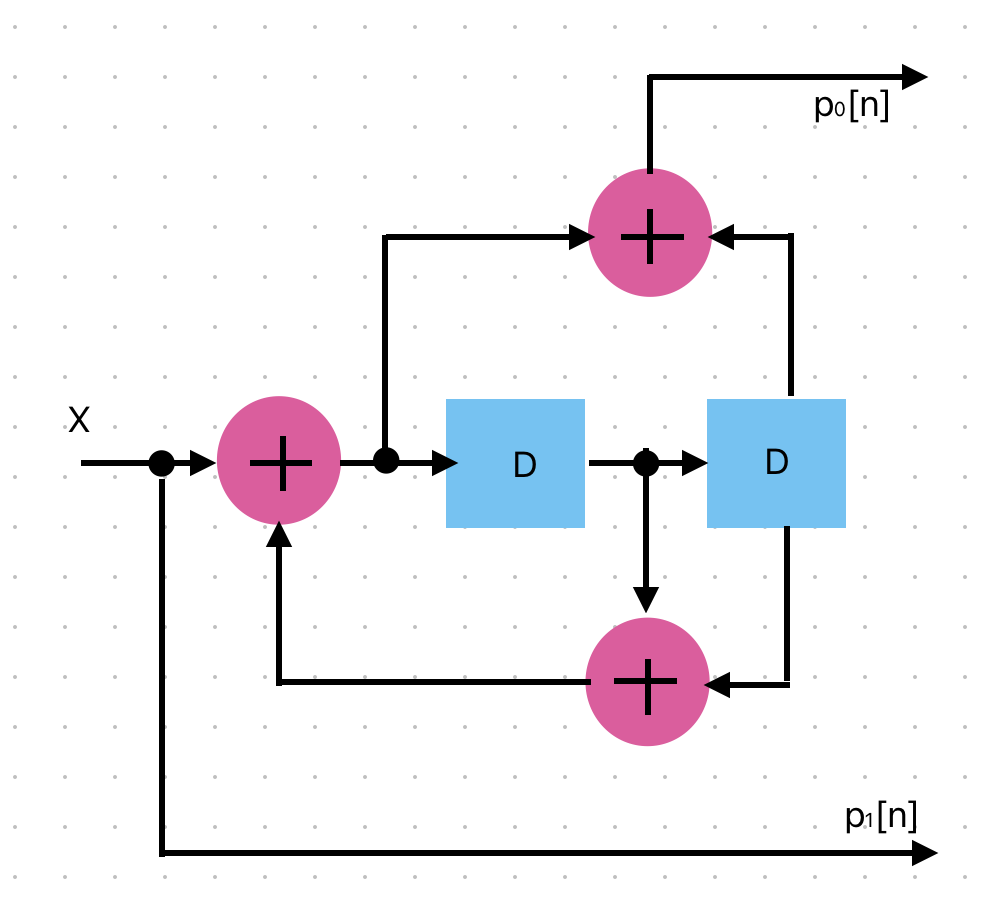
\includegraphics[width=0.6\textwidth]{Figs/Conv_RSC.png}
    \caption{Caption}
    \label{fig:Conv_RSC}
\end{figure}

The following is an extremely simple recursive systematic convolutional code. 

\begin{example}
    \textbf{Accumulator.} Figure~\ref{fig:accumulator} shows a rate \(1/2\) recursive systematic convolutional code. Assuming the input bits are \(x_1, x_2, x_3, \cdots, \), and output parity bits are \(y_1, y_2, y_3, \cdots\), then we have 
    \begin{align*}
        y_1 &= x_1 \\
        y_2 &= x_1 + x_2 \\
        y_3 &= x_1 + x_2 + x_3 \\
        \vdots \\
        y_n & = \sum_{i=1}^{n} x_i
    \end{align*}
    Such a convolutional code is called as an accumulator. In modulation, it is also commonly used as a pre-coder. The transfer function is \(\frac{1}{1+D}.\)
    
\begin{figure}[h]
    \centering
    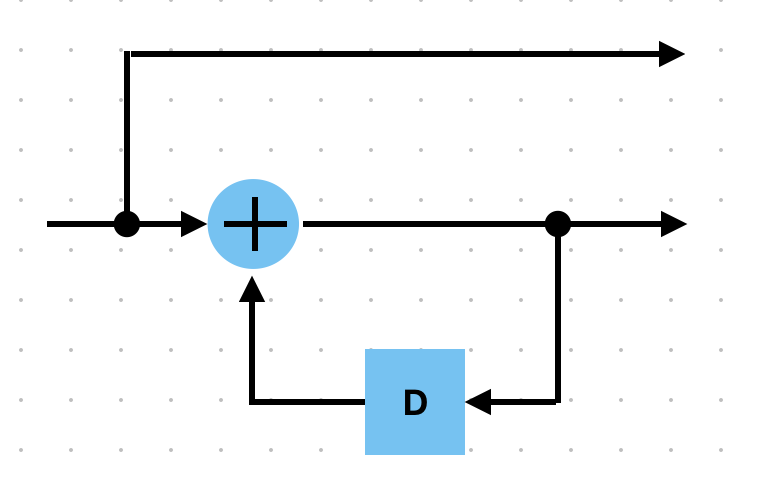
\includegraphics[width=0.6\textwidth]{Figs/Accumulator.png}
    \caption{An accumulator}
    \label{fig:accumulator}
\end{figure}

\end{example}


\subsection{Transfer Function of RSC}
The transfer function of the code defined in Fig~\ref{fig:Conv_RSC}.
We will introduce the variable \(s[n]\) to represent the value right before first register. Then we have the following equations: 
\begin{align*}
s[n] &= x[n] + s[n-1] + s[n-2] \nonumber\\
p[n] &= s[n] + s[n-2]
\end{align*}
Applying the \(z\)-transform to the two equations, we have 
\begin{align*}
S(1+D + D^2) &= X, \\
P &= S(1 + D^2).
\end{align*}
Canceling \(S\) in the above two equations gives us the transfer function: 

\begin{align}
\frac{P}{X} = \frac{1+D^2}{1+ D + D^2} \label{eq:RSCTransfer}
\end{align}

Compared with a non-recursive convolutional code, the transfer function of a recursive convolutional code has a non constant denomintor function. This provides the feedback loop.




\newpage

%\Lecturer{Hui Jin}
\Contributor{}
\LectureNumber{07}
\LectureDate{DATE}
\LectureTitle{Convolution Codes - Viterbi Decoding}

\lstset{style=mystyle}

	\MakeScribeTop

%#############################################################
%#############################################################
%#############################################################
%#############################################################

\section{Introduction}
If bit streams are encoded by a convolutional code, how do we find the correct codeword \(c\) given a received vector \(y\) which is a noisy version of a codeword? As noises are stochastic, finding the correct codeword is not guaranteed; instead our task is to find the most likely codeword.

For convolutional coding, there exists a low complexity  decoding algorithm, called Viterbi decoding, that guarantees to find the maximum likelihood codeword. It should be noted that even though Dr. Andrew Viterbi proposed the algorithm in 1967, it was not until six years later in 1973 that David Forney proved its optimality. 

In this lecture we shall describe this amazing algorithm. We will learn that Viterbi decoding is really a dynamic programming algorithm applied to a Markov tree process; the Markov tree corresponds to the trellis structure of the convolutional code.   

But before we discuss the Viterbi decoding, we describe a hard decision decoder. On the BSC channel, it is the optimal decoder. On the AWGN channel, it is a simplied version of the optimal Viterbi decoder.




\section{Maximum Likelihood Decoder}
The quantity \(p(y|c)\) represents the probability of receiving the vector \(y\) given that codeword \(c\) is transmitted. A Maximum Likelihood Decoder chooses the codeword such that this probability is maximized. 

If we assume the channel is memoryless, then for each transmitted bit, the noise generated by the channel is independent. That is to say
\begin{equation}
p(y|c) = \prod_{i=1}^{n}p(y_i|c_i) \label{eq:pyc}
\end{equation}
where \(c_i\) represents the block of parity bits transmitted at the \(i\)th input block, and \(y_i\) represents the block of received value after the channel if \(c_i\) is transmitted. Note that each block of parity bits \(c_i\) itself is a vector, consisting of \(r\) bits, i.e. \(c_i =c_{i}^{1}c_{i}^{1}\cdots c_{i}^{r}.\) Similarly, the block of the received value is a vector of length 
\(r\) as well: \(y_i = y_{i}^{1}y_{i}^{2}\cdots y_{i}^{r}\). Even though Eq.~\ref{eq:pyc} can be further factored into as \(p(y_i|c_i) = \prod_{j=1}^{r}p(y_i^{j}|c_i^{j})\), we hold off using this lest of unnecessary cluttering. We will use it in Section 3. 


Our maximum likelihood decoder chooses the codeword \(c\) such that the probability \(p(y|c)\) is maximized. 
\begin{equation}
    c_{ML} = \argmax_{c} p(y|c) = \argmax_{c=c_1, c_2, \cdots, c_n}  \prod_{i=1}^{n}p(y_i|c_i) \label{eq:MLDecoder}
\end{equation}

An intuitive understanding of the ML decoder is: on the trellis we want to find the path, which corresponds to a codeword, such that the probability of that path given received vector \(y\) is the largest. The decoding capability of convolutional codes comes from the fact that the distances between valid paths can be large. This is essentially the free distance property of the convolutional codes.  

\section{A hard decision decoder}


\section{A soft decision Decoder}
\subsection{Log-likelihood}
Since logrithm is a monotonical function, Eq~(\ref{eq:MLDecoder}) is equivalent to 
\begin{align}
    c_{ML} &= \argmax_{c} \log p(y|c) \nonumber \\ 
           &= \argmax_{c=c_1, c_2, \cdots, c_n} \log \prod_{i=1}^{n}p(y_i|c_i) \nonumber \\
           &= \argmax_{c=c_1, c_2, \cdots, c_n} \sum_{i=1}^{n} \log p(y_i|c_i) \label{eq:ML_Viterbi}
\end{align}


\subsection{Normalization and Log-likelihood Ratio}
We also realize that subtracting a constant from each term in Eq.~\ref{eq:ML_Viterbi} does not change the argmax. A neat trick to simplify the decoder is to subtract \(\log p(y_i|\bf{1})\) in the \(i\)-th sum, here \(\log p(y_i|\bf{1})\) represents the log-likeliood of receiving \(y_i\) given the all-one vector is transmitted in the \(i\)-th block. (It does not matter we use which transmitted vector as the base; we choose all one vector due to its simplicity in description.) 

\begin{align}
    c_{ML} &= \argmax_{c=c_1, c_2, \cdots, c_n} \sum_{i=1}^{n} (\log p(y_i|c_i) - \log p(y_i|0) \nonumber ) \\
    &=\argmax_{c=c_1, c_2, \cdots, c_n} \sum_{i=1}^{n} \log \frac{p(y_i|c_i)}{p(y_i|\bf{1})} \label{eq:CovnCML}
\end{align}

The quantity \( \log \frac{p(y_i|c_i)}{p(y_i|\bf{1})} \) is known the log-likelihood ratio between any other branch and the branch that has the all one transmitted bits. This trick is useful to remove the constant in  \(p(y_i|c_i)\); and it also nicely limits the data range in actual software/hardware implementation.

\begin{example}
On the Binary Symmetric Channel, assuming the two transmitted parity bits are \(c_i = 01\), the received vector is \(y_i = 11\), then we have 
\[p(y_i|c_i) = p(1-p),\]
and the log-likelihood is 
\[\log p(y_i|c_i) = \log(p(1-p)),\]
and the normalized log-likelihood ratio is

\begin{align*}
&\log \frac{p(y_i|c_i)}{p(y_i|11)}) \\ &= \log \frac{p(1-p)}{(1-p)(1-p)} \\
&=\log \frac{p}{1-p}.
\end{align*}

\end{example}

\begin{example}
On the AWGN Channel with Gaussian noise \(N(0, \sigma^2)\), assuming the two transmitted parity bits are \(c_i = 01\), the received vector is \(y_i = y_0y_1\), then we have
\[p(y_i|c_i) = \frac{1}{2\pi\sigma^2} \exp[-\frac{(y_0-1)^2+(y_1 + 1)^2}{2\sigma^2}],\]
and the log-likelihood is 
\[\log p(y_i|c_i) = \log(\frac{1}{2\pi\sigma^2}) -\frac{(y_0-1)^2+(y_1 + 1)^2}{2\sigma^2} ,\]
and the normalized log-likehood ratio is
\begin{align*}
&\log \frac{p(y_i|c_i)}{p(y_i|11)})\\ &= -\frac{(y_0-1)^2+(y_1 + 1)^2}{2\sigma^2} + \frac{(y_0+1)^2+(y_1 + 1)^2}{2\sigma^2} \\ 
&= \frac{2y_0}{\sigma^2}
\end{align*}
This last expression is surprisingly simple. And it makes intuitive sense. A positive \(y_0\) indicates the transmitted bit \(c_0\) is more likely to be \(0\), as the branch metric is \(\log \frac{p(y_0|0)}{p(y_0|1)}\). A negative says otherwise. 
\end{example}



\section{Branch Metric}
Let us define the \(i\)th branch metric to be 
\begin{equation}
  B_i(c_i) = \log \frac{p(y_i|c_i)}{p(y_i|\bf{1})} \label{eq:BranchMetric}
\end{equation}

Therefore, the maximum likelihood decision in Eq.~\ref{eq:CovnCML} turns to:
\begin{align}
    c_{ML}
    &=\argmax_{c=c_1, c_2, \cdots, c_n} \sum_{i=1}^{n} \log B_i(c_i) \label{eq:ConvBranchML} 
\end{align}
We will stamp the branch metric on the trellis and now the trellis graph has weights between the \(i\)-th state and the \((i+1)\)-state, for any pair of valid states. 

Let us look at two examples, both the binary symmetric channel case and the AWGN channel case. 

The maximum likelihood decoding problems becomes the problem of finding the maximum weight path along this trellis tree.   

Shed in this light, the optimal decision problem changes to a well known approach - dynamic programming! 

\section{Dynamic Programming}
Let us denote the trellis states as \(0, 1, \ldots, 2^K-1\), where \(K\) is the constraint length. In our example, \(K=2\), and the states are \(0, 1, 2, 3\).

The maximum likelihood decoded codeword corresponds to the path from state \(0\) at time \(t=1\) to any final state \(s\) at time \(t=n\) with the maximum sum of branch metrics. If we find the maximum path, then the associated path correspond to the Maximum Likelihood codeword. So our problem is really about the maximum path branch: 
\begin{align}
    B_{ML} &=\max_{c=c_1, c_2, \cdots, c_n} \sum_{i=1}^{n} \log B_i(c_i) \label{eq:ConvBranchML} 
\end{align}

But the maximum sum of branch metrics at time \(t=n\) can be decomposed to the maximum sum of branch metrics at time \(t=n-1\) and the branch metric at time \(t=n\). That is the basic principle of dynamic programming.

Formally, let us define the sum of a partial path, from state \(0\) at time \(t=1\) to a state \(s\) at time \(t=j\) as the cumulative branch metric (CB):
\begin{equation*}
    CB_{j}(s) = \max_{c=c_1, c_2, \cdots, c_j }\sum_{i=1}^{n} \log B_i(c_i),
\end{equation*}
where the ending state of \(c_1, c_2, \cdots, c_j\) is \(s\).

Clearly \(B_{ML} = \max_s CB_{n}(s).\) To compute \(CB_{j}(s)\), we rely on the following insight: 
\begin{theorem}
For a state \(s\), let \(P(s)\) be the set of states that can transit to \(s\). For state \(c' \in Pre(s)\), let \(c(s',s)\) be the coded bits generated as state \(s'\) transit to \(s\). With that definition, we have  
\begin{equation*}
    CB_j(s) = \max_{s' \in P(s)} (CB_{j-1}(s') + B_j(c(s',s))
\end{equation*}    
\end{theorem}
\begin{proof}
    It is almost evident if we look at the trellis. 
\end{proof}

\section{Put it together - the Viterbi Algorithm}
As described, the Viterbi algorithm is straightforward: 
\begin{itemize}
    \item calculate the branch metrics
    \item forward path dynamic programming
    \item trace back the maximum path to get the codeword
\end{itemize}


We will look at the trellis structure in figure. 

The following examples will reinforce our understanding. Costello book? Wicker book?  

\begin{example}
    
\end{example}

\section{Varying the code rate}
We can achieve different code rate through puncturing. 


\section{The complexity of Viterbi Decoding}
It only requires a forward path. At each time step, we have \(2^K \times M\) computations, total operations is \(n M 2^K\). 

Storage requirement: about \(2^K\) branch metrics and record the codeword. 


\section{The performance of Convolution Codes}

The 3dB performance gap from the Shannon limit. 


\newpage

%\Lecturer{Hui Jin}
\Contributor{}
\LectureNumber{07}
\LectureDate{DATE}
\LectureTitle{Turbo Codes}

\lstset{style=mystyle}

	\MakeScribeTop

%#############################################################
%#############################################################
%#############################################################
%#############################################################

\section{Introduction}
In late 1980s, there was a sense that "channel coding" was a dead field. Algebraic codes like Reed Solomon codes and convolutional codes had been studied thoroughly. They showed good performance but fell well short of the Shannon limit.  In fact, the best codes usually required more than twice the transmitting power that Shannon’s law said was necessary to reach a certain level of reliability. The gap between the practical and the ideal, measured in decibels — a ratio between the signal level and the noise level on a logarithmic scale — was about $3.5$ dB. To chip away at it, engineers needed more elaborate codes. On other channels, like block fading channels, the gap was even wider. But there seemed a dead end for new ideas. A lot of researchers believed that the $3$dB barrier to the Shannon limit was unbreakable.


Then, completely out of the blue, a revolution in coding theory occurred in 1993. On the IEEE International Communications Conference, French researchers Berrou and Glavieux presented a new type of codes - turbo codes. The researchers claimed that these codes could achieve within $1$dB of the Shannon capacity. On this outlandish claim, many in the conference were skeptical, partially because at the time the authors of the paper were largely unknown in the field. Few people bothered to read the paper, suspecting the authors made some calculation error in the units of signal-to-noise ratio. But once other researchers began to validate the results independently, a massive research effort was soon underway with the goal of explaining and, better yet, enhancing the remarkable performance of turbo codes. Much of this research focused on improving the practicality of turbo codes, which, as will be dis- cussed shortly, have some peculiarities that make implementation less than straightforward.

By the end of the 1990s, the virtues of turbo codes were well known, and they began to be adopted in various systems. Now they are incorporated into standards used by NASA for deep space communications (CCSDS), and both third-generation cellular standards (UMTS and cdma2000).


\section{Turbo Code Structure}
The original turbo code was the parallel concatenated convolutional code (PCCC). 

\subsection{Recursive Systematic Convolutional Code}
In inventing Turbo codes, Dr. Berrou was also the first one to introduce Recursive Systematic Convolutional Codes. 

The RSC encoder of this conventional convolutional encoder is represented 12
as \(G=[1, g / g ]\) where the first output (represented by g ) is fed back to the input.  Figure \ref{fig:Conv_RSC} shows the resulting 
RSC encoder.

\begin{figure}[h]
    \centering
    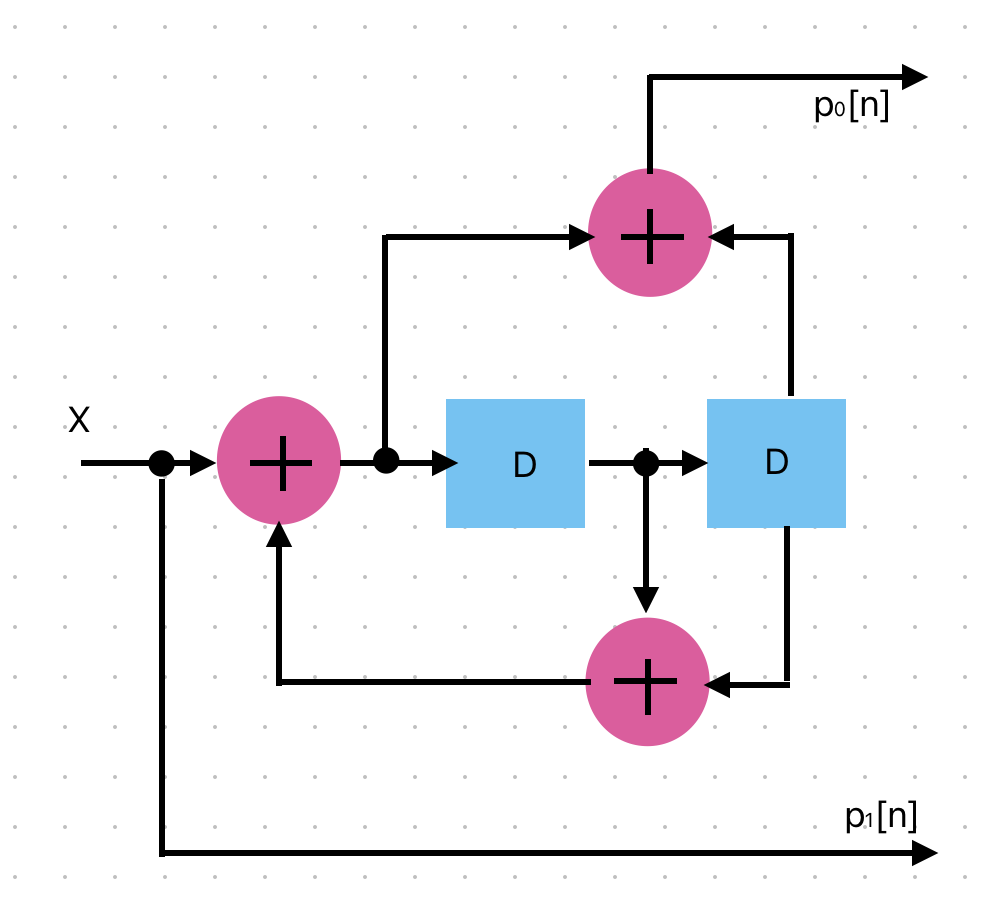
\includegraphics[width=0.6\textwidth]{Figs/Conv_RSC.png}
    \caption{Caption}
    \label{fig:Conv_RSC}
\end{figure}

\subsection{Transfer Function of RSC}
The transfer function of the code defined in Fig~\ref{fig:Conv_RSC}.
We will introduce the variable \(s[n]\) to represent the value right before first register. Then we have the following equations: 
\begin{align*}
s[n] = x[n] + s[n-1] + s[n-2] \nonumber
p[n] = s[n] + s[n-2]
\end{align*}
Applying the \(z\)-transform to the two equations, we have 
\begin{align*}
S(1+z + z^2) &= X, \\
P &= S(1 + z^2).
\end{align*}
Canceling \(S\) in the above two equations gives us the transfer function: 

\begin{align}
\frac{P}{X} = \frac{1+z^2}{1+ z + z^2} \label{eq:RSCTransfer}
\end{align}

Compared with a non-recursive convolutional code, the transfer function of a recursive convolutional code has a non constant denomintor function. This provides the feedback loop.

\subsection{Turbo Code Structure}

\subsection{Encoding}

\subsection{Puncturing}

structure and the encoding algorithm. 
\section{Interleaver Design}
\subsection{Random Interleaver} 
\subsection{S-random interleaver}

\section{Serial Turbo Code}


\section{Irregular Turbo Code}

Algebraic construction. 



\newpage

%\Lecturer{Hui Jin}
\Contributor{}
\LectureNumber{08}
\LectureDate{DATE}
\LectureTitle{Turbo Codes Decoding and Design}

\lstset{style=mystyle}

	\MakeScribeTop

%#############################################################
%#############################################################
%#############################################################
%#############################################################

\section{Introduction}
The key innovation of turbo codes is how they use the likelihood data to reconcile differences between the two decoders. Each of the two convolutional decoders generates a hypothesis (with derived likelihoods) for the pattern of m bits in the payload sub-block. The hypothesis bit-patterns are compared, and if they differ, the decoders exchange the derived likelihoods they have for each bit in the hypotheses. Each decoder incorporates the derived likelihood estimates from the other decoder to generate a new hypothesis for the bits in the payload. Then they compare these new hypotheses. This iterative process continues until the two decoders come up with the same hypothesis for the m-bit pattern of the payload, typically in a couple dozen cycles.

\section{Maximum A Posteriori Decoder of Convolutional Codes}
In the lecture of Convolutional Code decoding, we described Maximum Likelihood Decoder, where the decoding decision is to choose the code \(c\) that maximizes the probability \(p(y|c)\). It corresponds to  
\begin{align}
    c_{ML} &= \argmax_{c} \log p(y|c) \nonumber \\ 
           &= \argmax_{c=c_1, c_2, \cdots, c_n} \log \prod_{i=1}^{n}p(y_i|c_i) \nonumber \\
           &= \argmax_{c=c_1, c_2, \cdots, c_n} \sum_{i=1}^{n} \log p(y_i|c_i) \label{eq:ML_Viterbi}
\end{align}
The maximum-likelihood decoder finds the whole sequence of information bits, thus the codeword, that maximizes the received sequence. The decoder admits a linear complexity Viterbi decoding algorithm because of the Markov tree property of the trellis structure. 

For the turbo codes with a concatenated convolution code, the maximum-likelihood decoder cannot be achieved with linear decoding complexity. Rather, the genius of the turbo code inventors lies at the iterative decoding method. The decoding algorithm treats the two convolution codes separately and decodes each one with the help of the other one. They showed with just a few iterative steps, the decoding performance is spectacular. 


 The iterative decoding algorithm works in successive fashion. We decode one convolution code first, obtaining the Maximum A Posteriori (MAP) soft decision of the information bits; then we use such MAP decision as prior, decoding the other convolution code, obtaining the MAP decision from that code. This new MAP decision is subsequently used to decode the first convolution code, starting the second decoding cycle. 

The fundamental decoding block is to obtain the MAP soft decision of the convolution code, given prior information. The algorithm is known as the BCJR algorithm, derived by Bahl, Cocke, Jelinek and Raviv in 1974. The BCJR algorithm is also known as the Forward-Backward algorithm. 

The BCJR algorithm gives the MAP decision on the individual information bits

\section{Turbo Decoding - BCJR Algorithm}

\subsection{A Priori and A Posteriori}
Let us consider a block or convolutional encoder described by a trellis, and a sequence
\(x = x_1x_2 ...x_N\) of \(N\) \(n\)-bit codewords or symbols at its output, where \(x_k\) is the symbol generated by the
encoder at time \(k\). The corresponding information or message input bit, \(uk\), can take on the values \(0\) or \(1\) with an a priori probability \(P(u_k)\), from which we can define the so-called log-likelihood ratio (LLR):

\begin{equation}
    L(u_k) = \ln \frac{P(u_k=1)}{P(u_k=0)}
\end{equation}

Suppose the coded sequence \(x\) is transmitted over a memoryless additive white gaussian noise
(AWGN)channel and  received as the sequence of \(nN\) real numbers \(y=y_1y_2...y_N\).
This sequence is delivered to the decoder and used by the decoder algorithm in order to estimate the original bit sequence \(u_k\). For which the algorithm computes the a posteriori log-likelihood ratio
\(L(u_k| y)\) , a real number defined by the ratio:
\begin{equation}
    L(u_k|y) = \ln \frac{P(u_k=1|y)}{P(u_k=0|y)}
\end{equation}

\subsection{MAP derivation}
We want to calculate \(L(u_k|y) = \ln \frac{P(u_k = 1|y)}{P(u_k = 0|y)}\). If \(L(u_k |y) > 0\), the decoder can make a hard decision that the bit
\(u_k = 1\) was sent, otherwise it will estimate \(u_k = 0\) was sent. Using our simple exemplary convolution code, the trellis has four states; from times k-1 and k there are \(8\) transitions between states \(S_{k-1} = s’\) and next states \(S_k = s\): four result from a \(0\) input bit (those drawn with a thick line) and the other four result from a \(1\) input bit. Each one of these transitions is due unequivocally to a known bit (just notice in the trellis if the branch line is solid or dashed). Therefore, the probabilities that \(u_k = 0\) or \(u_k = 1\), given our knowledge of the sequence \(y\), are equal to the probabilities that the transitions (s’,s) between states correspond to a solid or a dashed line, respectively. Since transitions are mutually exlusive – just one can occur at a given time – the probability that any one of them occurs is equal to the sum of the individual probabilities, that is,
\begin{align*}
    P(u_k=1|y) &= \sum_{s', s, u_k=1}P(s', s|y),\\
    P(u_k=0|y) &= \sum_{s', s, u_k=0}P(s', s|y).  
\end{align*}


\section{Turbo Decoding as an instance of Belief Propagation}



\newpage

%\input{Lectures_Classical/LDPCCodes}
\newpage

%\input{Lectures_Classical/LDPCCodesDesign}
\newpage

%\input{Lectures_Classical/TurboLikeCodes}
\newpage

%\Lecturer{Hui Jin}
\Contributor{}
\LectureNumber{13}
\LectureDate{DATE}
\LectureTitle{Introduction to Quantum Information}

\lstset{style=mystyle}


	\MakeScribeTop

%#############################################################
%#############################################################
%#############################################################
%#############################################################

\section{Introduction}
[J Preskill] In quantum theory, the act of acquiring information about a physical system inevitably disturbs the state of the system. There is no counterpart of this limitation in classical physics.

That acquiring information causes a disturbance is also connected with another essential distinction between quantum and classical information: quantum information cannot be copied with perfect fidelity. If we could make a perfect copy of a quantum state, we could measure an observable of the copy without disturbing the original and we could defeat the principle of disturbance. On the other hand, nothing prevents us from copying classical information perfectly.

These properties of quantum information are important, but the really deep way in which quantum information differs from classical information emerged from the work of John Bell. Bell showed that quantum information can be (in fact, typically is) encoded in nonlocal correlations between the different parts of a physical system, correlations with no classical counterpart. 

The study of quantum information as a coherent discipline began to emerge in the 1980’s, and it has blossomed in the 1990’s.

\section{The Qubit}
The unit of classical information is the bit, which can take either one of two values: \(0\) or \(1\). The corresponding unit of quantum information is the quantum bit or qubit. The qubit is a vector in a two dimensional complex vector space with inner product (A Hilbert Space of dimension of \(2\)). We can call the elements of an orthonormal basis in this space \(\ket{0}\) and \(\ket{1}\), by using the Dirac's ket notation. Conventionally, the orthonormal basis \(\ket{0}\) and \(\ket{1}\) are taken to be
\begin{align*}
    \ket{0} = \begin{bmatrix}
           1 \\
           0 
         \end{bmatrix}
    , \;\;\;
    \ket{1} = \begin{bmatrix}
           0 \\
           1 
         \end{bmatrix}.
  \end{align*}
  
  Then a normalized vector can be represented
\[\ket{\psi} = \alpha \ket{0} + \beta \ket{1} =  \begin{bmatrix}
           \alpha \\
           \beta 
    \end{bmatrix},
\] 
where \(\alpha, \beta \in C\) and \(|\alpha|^2 + |\beta|^2 = 1\). This defines a qubit, a superposition of the two base vectors. We can perform a measurement that projects \(\ket{\phi}\) onto the basis \(\ket{0}\), \(\ket{1}\). The outcome of the measurement is not deterministic — the probability that we obtain the result \(\ket{0}\) is \(|\alpha|^2\) and the probability that we obtain the result \(\ket{1}\) is \(|\beta|^2\). Once measured, superposition of the qubit is removed and the qubit collapsed to the classical bit. 

Nature operates in the quantum world, and stores information in a superposition way. The most revealing observation is the double slit experiment. 

Two important superposition states are
\[\frac{1}{\sqrt{2}}(\ket{0} +\ket{1}) \]
and
\[\frac{1}{\sqrt{2}}(\ket{0} - \ket{1}) \]
These will come up repeatedly. They are often referred to as the "\(\ket{+}\)" and "\(\ket{-}\)" states, for obvious reasons. If \(\ket{0}\) and \(\ket{1}\) are vectors pointing along the \(x\) and \(y\) axes, then \(\ket{+}\) and \(\ket{-}\) are the diagonal vectors. Note that \(\ket{+}\) and \(\ket{-}\) are orthogonal to one another and act in all respects like an alternative pair of basis states. 

\subsection{Exponential Dimension of \(n\)-qubits}
We know \(N\) classical bits can take \(2^N\) possible values; the system of \(N\) classical bits has dimension of \(N\) as we can use a binary string of length \(N\) to describe it. A configuration of \(N\) qubits, on the other hand, requires \(2^N\) complex numbers for a complete description. Therefore the dimension of N-qubits is \(2^N\), growing exponentially with the number of qubits.   

For instance, to describe a configuration of \(100\) classical bits, we need \(100\) bits; to describe a configuration of \(100\) qubits in the classical world, we need \(2^{100}\) complex numbers. Here lies the difficulty of using classical computation systems to simulate a quantum world.

\subsection{Multiple Qubits Tensor Product}
The tensor product (or Kronecker product) is used to combine quantum states. The combined state for a qubit register is the tensor product of the constituent qubits. The tensor product is denoted by the symbol 
\(\otimes\).
The vector representation of two qubits is:
\[
\ket{\psi} = v_{00}\ket{00} + v_{01}\ket{01} + v_{10}\ket{10} + v_{11}\ket{11}
\rightarrow {\begin{bmatrix}v_{00}\\v_{01}\\v_{10}\\v_{11}\end{bmatrix}}.
\]

\section{Linearity of Quantum Mechanics}
The linearity of quantum mechanics (QM) is a fundamental feature. This linearity does not depend on the particular object under study, provided it is sufficiently isolated from anything else. It is naturally reflected in the superposition principle and entails the “quantum essentials” interference and entanglement, without which modern applications of QM, e.g. in precision measurement and information technologies, and the ongoing study of the foundations of QM would not be the same.

In our discussion, we assume all manipulation of the qubits are through unitary operations, which are linear. Thus we can analyze a quantum circuit first using the base vectors, and then for the general qubits, the effect can be obtained by superposition principle. This approach is fundamental in our analysis. 

\section{The Quantum Logic Gates}
In quantum computing and specifically the quantum circuit model of computation, a quantum logic gate (or simply quantum gate) is a basic quantum circuit operating on a small number of qubits. Quantum logic gates are the building blocks of quantum circuits, like classical logic gates are for conventional digital circuits.

Quantum gates are unitary operators, and can be described unitary matrices. In the following, we describe the building blocks of these quantum gates.

A gate that acts on \(n\) qubits is represented by a \(2^n \times 2^n\) unitary matrix. 

\subsection{Quantum gates on one-qubit}
The Pauli matrices are a set of three \(2 \times 2\) complex matrices that are Hermitian and unitary. We manipulate qubits by applying Pauli matrices; they are also how the environment introduces noise onto the qubits. 

\paragraph{X} 
Pauli Matrix \(X\) swaps the base states:
\begin{align*}
    X \ket{0} &= \ket{1} \\
    X \ket{1} &= \ket{0} 
\end{align*}
Based on such transformation, we know that 
$$X = \begin{bmatrix}
    0 & 1 \\
    1 & 0 
\end{bmatrix}$$

By linearity of quantum states, we have for a general qubit \(\ket{q}\), 
\begin{align*}
    X \ket{q} = X (\alpha \ket{0} + \beta \ket{1}) &= \alpha \ket{1} + \beta \ket{0}
\end{align*}
Equivalently, this can be represented by the unitary matrix operation \(X\begin{bmatrix}
           \alpha \\
           \beta 
    \end{bmatrix} = \begin{bmatrix}
           \beta \\
           \alpha 
    \end{bmatrix} 
    \).
\paragraph{Z} 
Pauli Matrix \(Z\) introduces a phase shift to the qubit:
\begin{align*}
    Z \ket{0} &= \ket{0} \\
    Z \ket{1} &= -\ket{1} \\
    Z (\alpha \ket{0} + \beta \ket{1}) &= \alpha \ket{0} - \beta \ket{1}
\end{align*}
Based on such transformation, we know that 
$$Z = \begin{bmatrix}
    1 & 0 \\
    0 & -1 
\end{bmatrix}$$

\paragraph{Y} Pauli matrix \(Y\) introduces a bit flip and a phase shift to a qubit: 
\begin{align*}
    Y \ket{0} &= i\ket{1} \\
    Y \ket{1} &= -i\ket{0} \\
    Y (\alpha \ket{0} + \beta \ket{1}) &= i(\alpha \ket{1} - \beta \ket{1})
\end{align*}
Based on such transformation, we know that 
$$Y = \begin{bmatrix}
    0 & -i \\
    i & 0 
\end{bmatrix}$$

The Pauli matrices are involutory, meaning that the square of a Pauli matrix is the identity matrix.
 \[X^2 = Y^2 = Z^2 = -iXYZ = I\] and \[ZX=-XZ = iY\]. 

\paragraph{Hadamard Matrix H} 
The Hadamard matrix \(H\) maps one normalized basis to another normalized basis: 
\begin{align*}
    H \ket{0} &= \frac{1}{\sqrt{2}}( \ket{0} + \ket{1}) = \ket{+} \\
    H \ket{1} &= \frac{1}{\sqrt{2}}( \ket{0} - \ket{1}) = \ket{-} \\
    H (\alpha \ket{0} + \beta \ket{1}) &= \alpha \ket{+} + \beta \ket{-}
\end{align*}
Based on such transformation, we know that 
$$H = \frac{1}{\sqrt{2}}\begin{bmatrix}
    1 & 1 \\
    1 & -1 
\end{bmatrix}$$


\subsection{Quantum gates on multi-qubits}
\paragraph{CNOT Gate}
The controlled NOT gate (or CNOT or CX) acts on 2 qubits, and performs the NOT operation on the second qubit only when the first qubit is \(\ket{1}\), and otherwise leaves it unchanged. With the convention of using the left qubit \(\ket{b_1}\) as the control bit in \(\ket{b_1b_2}\), we have

\begin{align*}
    CX \ket{00} &= \ket{00} \\
    CX \ket{01} &= \ket{01} \\
    CX \ket{10} &= \ket{11} \\
    CX \ket{11} &= \ket{10} 
\end{align*}

 Based on such transformation, we know that it is represented by the Hermitian unitary matrix:
$$CX = \begin{bmatrix}
    1 & 0 & 0 & 0  \\
    0 & 1 & 0 & 0  \\
    0 & 0 & 0 & 1  \\
    0 & 0 & 1 & 0   
\end{bmatrix}$$

The quantum circuit of the CNOT gate is depicted in Figure~\ref{fig:cnot}
\begin{figure}[h]
    \centering
    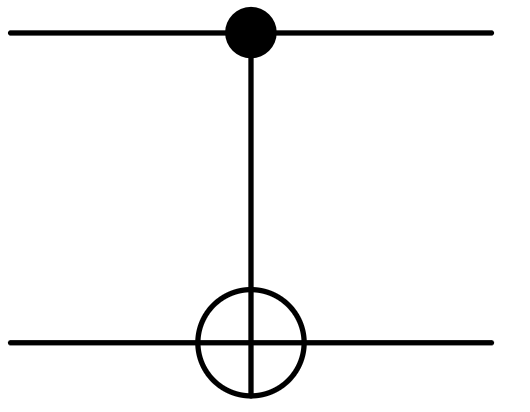
\includegraphics[width=0.3\textwidth]{Figs/cnot.png}
    \caption{CNOT gate performs the NOT operation on the second qubit only when the first qubit is \(\ket{1}\), and otherwise leaves it unchanged. }
    \label{fig:cnot}
\end{figure}


\paragraph{SWAP Gate}
The swap gate (SWAP) performs the swap operation on the two qubits; we have

\begin{align*}
    SWAP \ket{00} &= \ket{00} \\
    SWAP \ket{01} &= \ket{10} \\
    SWAP \ket{10} &= \ket{01} \\
    SWAP \ket{11} &= \ket{11} 
\end{align*}
Based on such transformation, we know that it is represented by the Hermitian unitary matrix:
$$CX = \begin{bmatrix}
    1 & 0 & 0 & 0  \\
    0 & 0 & 1 & 0  \\
    0 & 1 & 0 & 0  \\
    0 & 0 & 0 & 1   
\end{bmatrix}$$

The quantum circuit of the SWAP gate is depicted in Figure~\ref{fig:swap}
\begin{figure}[h]
    \centering
    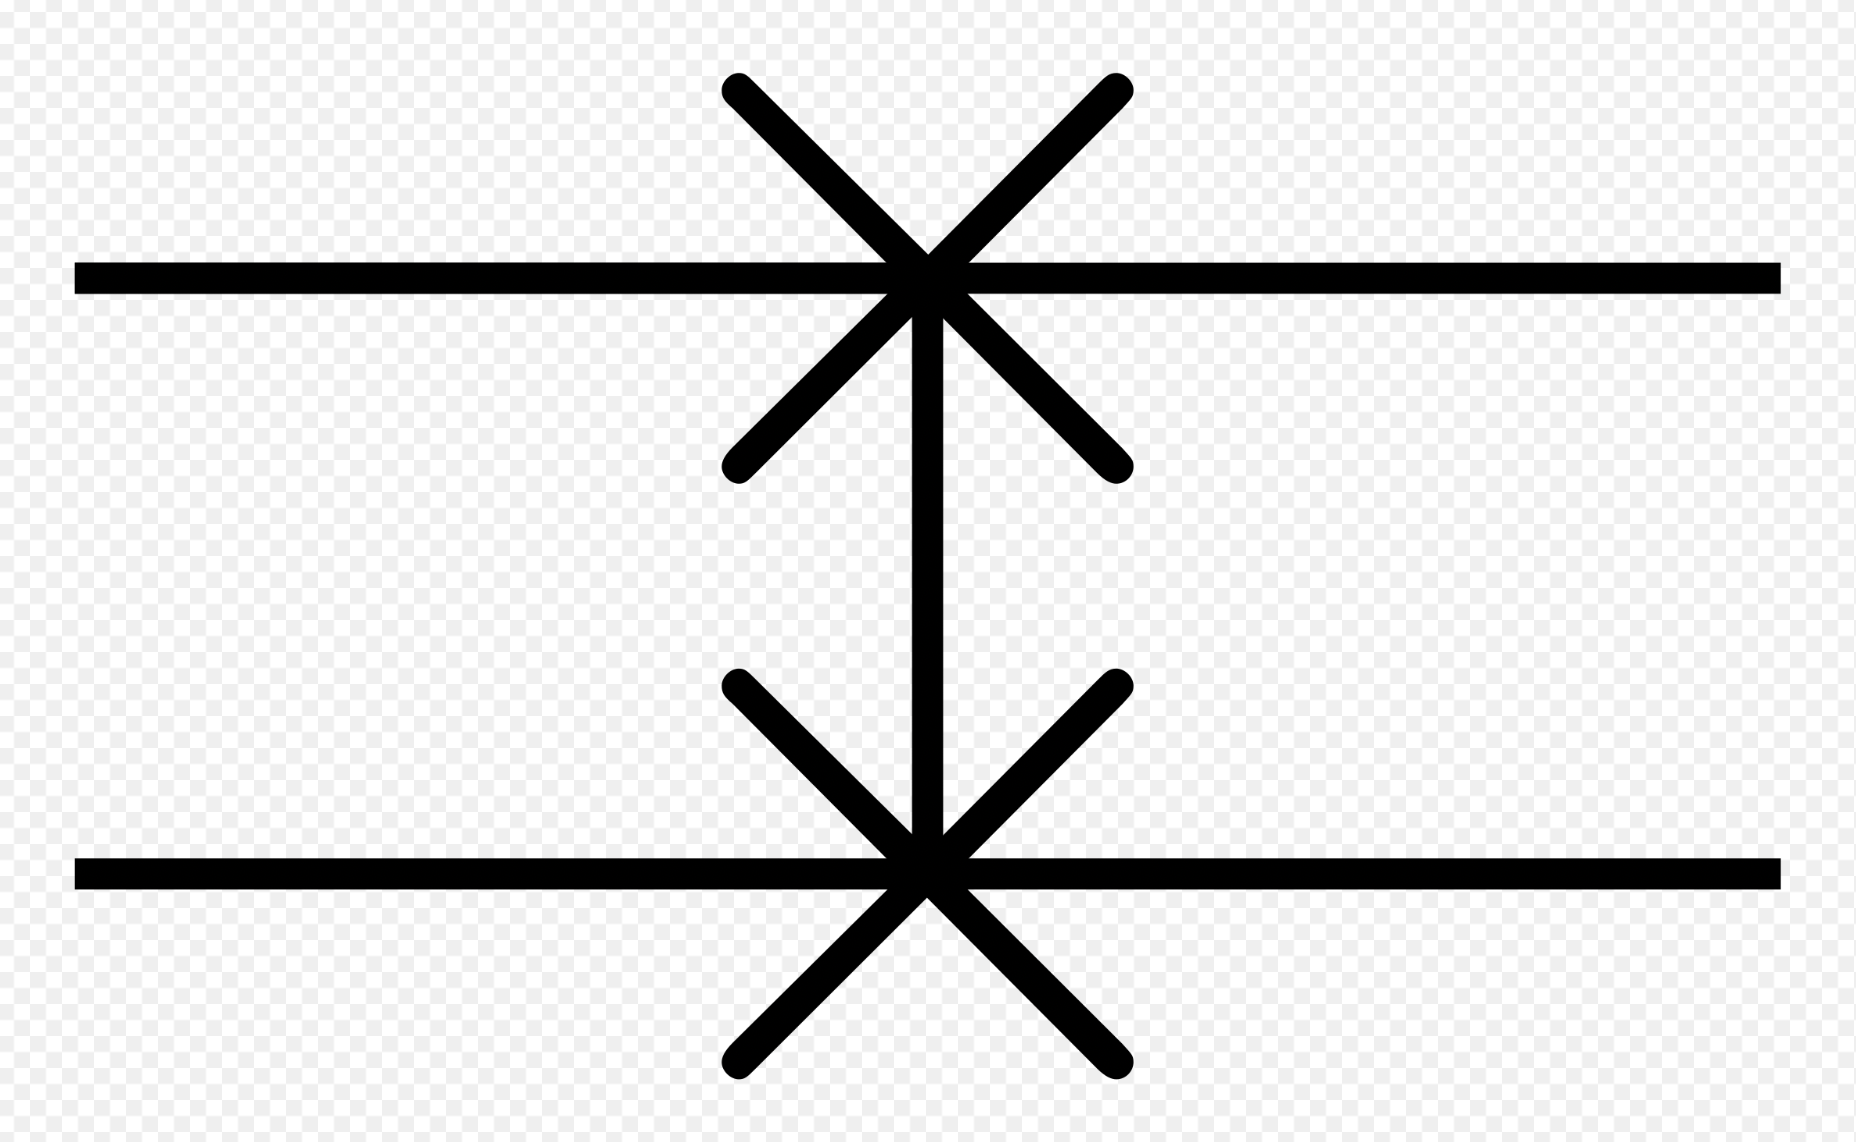
\includegraphics[width=0.3\textwidth]{Figs/swap.png}
    \caption{SWAP gate performs the swap of the two qubits. }
    \label{fig:swap}
\end{figure}


\paragraph{Toffoli Gate}
The quantum Toffoli gate is defined for \(3\) qubits. It is an extension of the CNOT gate; it performs the NOT operation on the third qubit if and only if the first two qubits are both \(\ket{1}\).

We have
\begin{align*}
    TOFF \ket{110} &= \ket{111} \\
    TOFF \ket{111} &= \ket{110} \\
    TOFF \ket{abc} &= \ket{abc} \; \; \text{all other three qubits}
\end{align*}

The quantum circuit of the Toffoli gate is depicted in Figure~\ref{fig:tofolli}
\begin{figure}[h]
    \centering
    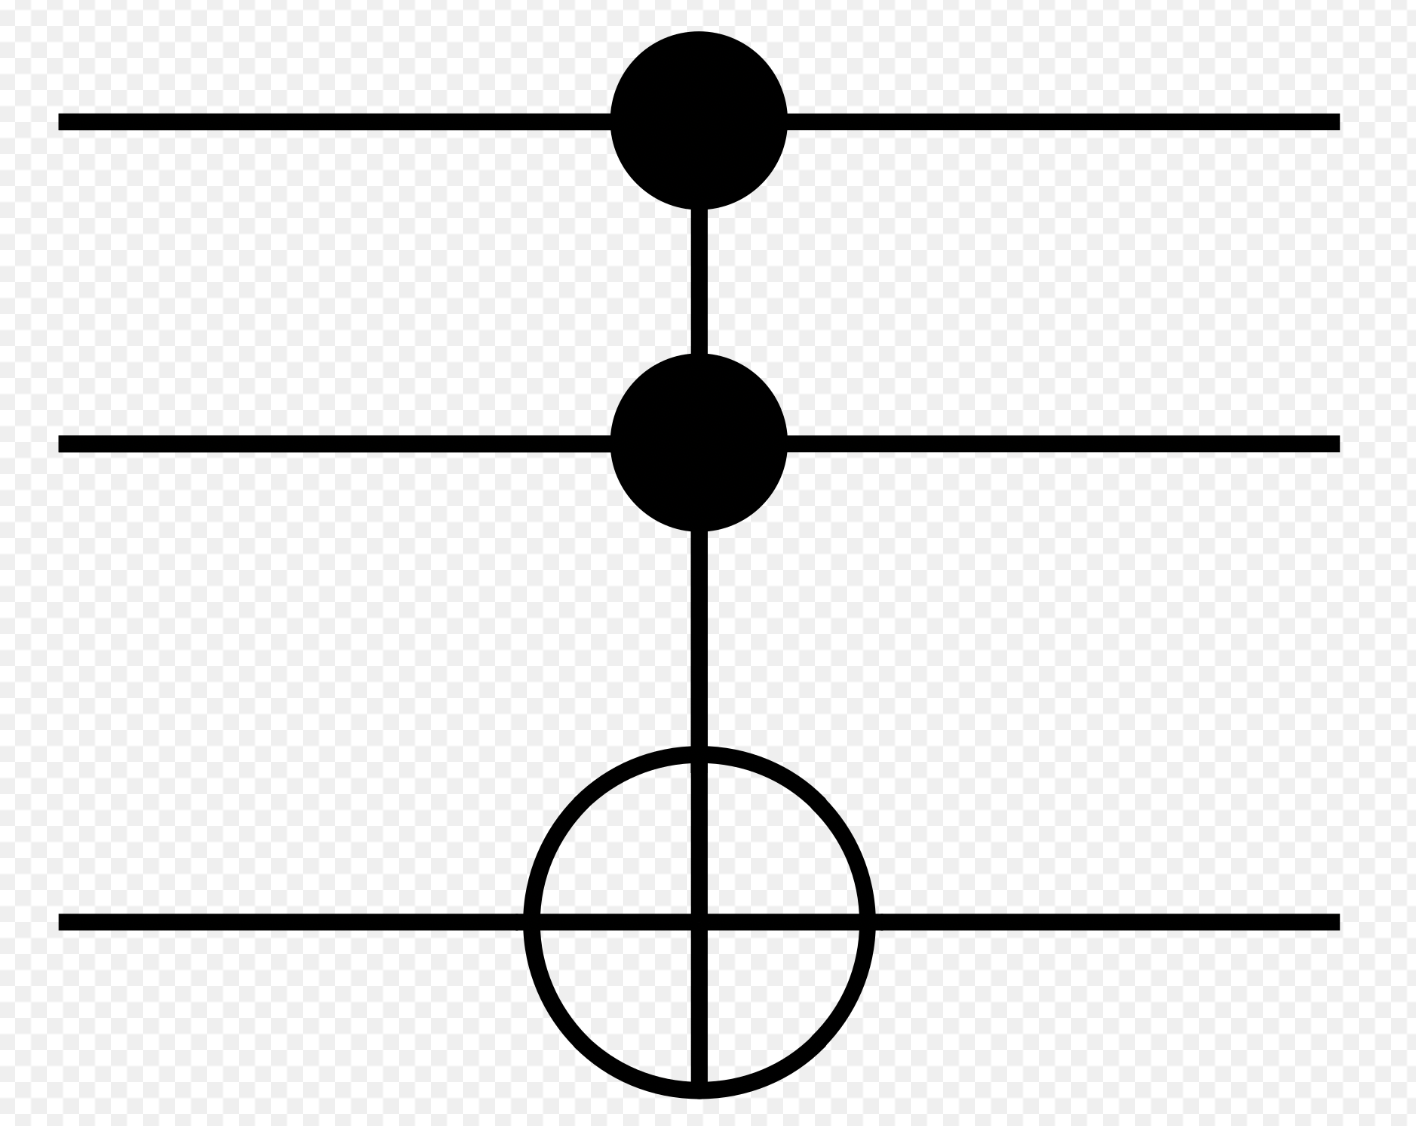
\includegraphics[width=0.3\textwidth]{Figs/Toffoli.png}
    \caption{Toffoli gate performs NOT operation on the third bit if and only both the first two qubits are \(\ket{1}\). }
    \label{fig:tofolli}
\end{figure}

\section{The standard ways to analyze a quantum circuit}
To analyze the output state of a quantum circuit, there are some standard approaches. 

The first common approach rests on the linear property of quantum circuit. If we know the output for every basis state, we know the operation matrix as each basis state corresponds to a column of the operation matrix. If fact, that is the basic approach for us to obtain the unitary matrix representation for the basic quantum gates. 

The second common approach is more for complicated circuits. With a concatenation of simple circuits, sometimes it is simpler to use the matrix multiplication to analyze the circuit.


\paragraph{break here}

\section{Some important quantum circuits}

\subsection{Repetition Circuit}
An important technique in classical coding is to use repetition. We can achieve a similar repetition using entanglement. 

It is easy to check in the CNOT gate, if we let the control qubit be \(\ket{x}\) and the second qubit be \(\ket{0}\), then the output qubits is \(\ket{xx}\). 


If the inputs are superposition: \(\alpha\ket{0}+ \beta\ket{1}\), then the quantum circuit will produce  
\[\alpha\ket{00} + \beta\ket{11}.\]

\begin{figure}[h]
    \centering
    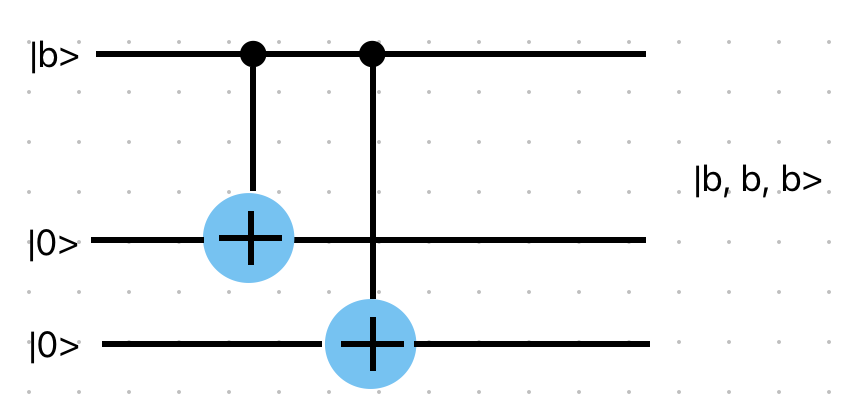
\includegraphics[width=0.6\textwidth]{Figs/QEC_Repeat.png}
    \caption{Qubit repetition through entanglement.}
    \label{fig:QEC_repeat}
\end{figure}

We can use the same control bit \(\ket{x}\) to control another NOT gate on another qubit \(\ket{0}\), like in Figure~\ref{fig:QEC_repeat} and produce another repeated qubit and the resulted output will be 
\[\alpha\ket{000} + \beta\ket{111}.\]


\subsection{Parity check circuit}
An important technique in classical coding is to use parity check bits. We can achieve a similar parity check qubits using entanglement. 

For example, Figure~\ref{fig:QECParity} shows the quantum circuit that takes in two base (\(\ket{0}\) or \(\ket{1}\)) qubits \(\ket{x}\) and \(\ket{y}\) and generate at the output entangled state \(\ket{x, y, x+y}\)

\begin{figure}[h]
    \centering
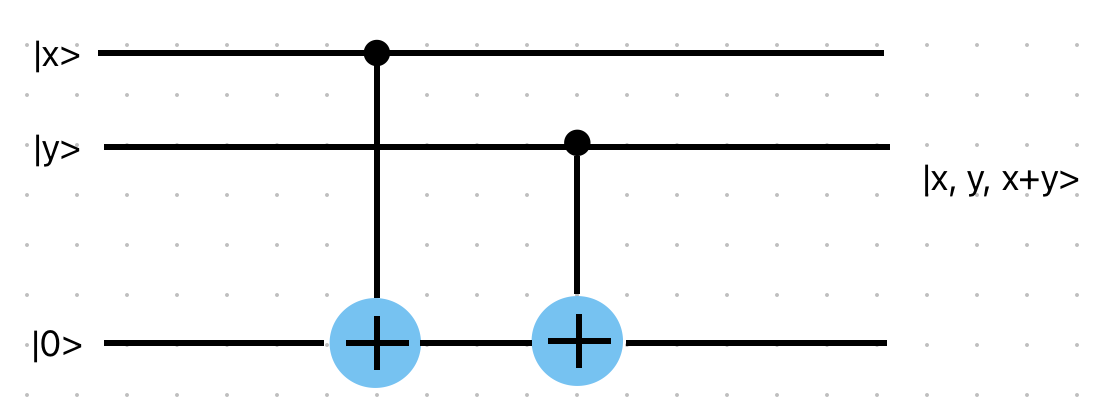
\includegraphics[width=0.75\textwidth]{Figs/QecParityCheck.png}
    \caption{Quantum circuit to parity check qubits through entanglement}
    \label{fig:QECParity}
\end{figure}

What if the inputs are superposition of \(\ket{0}\) and \(\ket{1}\), for example \(\ket{x} = \ket{y} = \ket{+}\), then the quantum circuit will produce at the output, by considering the base states, 
\[\frac{1}{2}(\ket{000} + \ket{011} + \ket{101} + \ket{110}).\]
As we see, in each of the base states generated, the binary representation of the qubits satisfies the parity check.

\subsection{The action of Hadamard Transformation}
We know that \(H\ket{0} = \frac{1}{2}\ket{+}\) and  \(H\ket{1} = \frac{1}{2}\ket{-}\). If we do Hadamard transformation to n-qubits in parallel, we can generate a uniform distribution on all possible \(n\)-bit base states. First, the transformed result on the all zero base vector is easy to see: 
\begin{lemma}
The action of \(H^{n}\) on n-qubit \(\ket{0^n}\) yields the transformation
\begin{align*}
H^{n}\ket{0^n} = \frac{1}{\sqrt{2^n}} \sum_{z=0}^{2^n-1} \ket{z}  
\end{align*}
\end{lemma}
\begin{proof}
\end{proof}


This result can be generalized to the transformation on any base vector: 
\begin{lemma}
The action of \(H^{n}\) on any n-qubit \(\ket{x}\) yields the transformation
\begin{align*}
H^{n}\ket{x} = \frac{1}{\sqrt{2^n}} \sum_{z} (-1)^{x\cdot z} \ket{z}     
\end{align*}

where \(z\) enumerates all possible \(n\)-bit combination and \(x\cdot z\) is a bit-wise dot-product. 
\label{lemma:HadamardAction}    
\end{lemma}

\begin{proof}
    We prove this by induction. 
\end{proof}

\subsection{Bell's States}
 We consider Hadamard gate and a CNOT gate as in Figure~\ref{fig:bell00}. Different combination of inputs will generate the four Bell's states. For example, in the figure the quantum circuit takes the two qubit input \(\ket{00}\) and transforms it to the first Bell state \(\ket{\phi^{+}}\). Explicitly, the Hadamard gate transforms \(\ket{00}\) into a superposition of \(\ket{+}\ket{0}\). This will then act as a control input to the CNOT gate, which only inverts the target (the second qubit) when the control (the first qubit) is \(1\). Thus, the CNOT gate transforms the second qubit as follows 
\(\frac {1}{\sqrt{2}}(\ket{00} + \ket{11})\).

\begin{figure}[h]
    \centering
    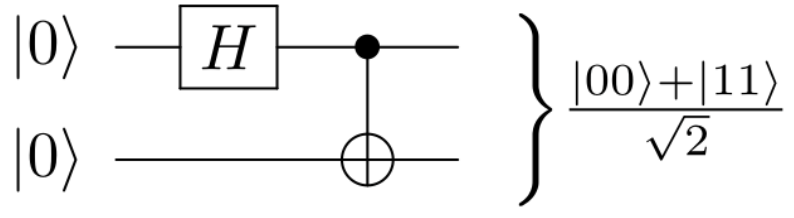
\includegraphics[width=0.5\textwidth]{Figs/BellState00.png}
    \caption{Quantum circuit to generate Bell state}
    \label{fig:bell00}
\end{figure}
Input \(\ket{10}\) will generate \(\ket{\phi^{-}}\) and so on.

 The Bell's states or EPR pairs are specific quantum states of two qubits that represent the simplest examples of quantum entanglement, a property that is essential in quantum computation. 




\section{The Magic of Quantum Algorithms}
The exciting new result that Shor found is that a quantum computer can factor in polynomial time, e.g., in time \(O(\ln n)^3\).

 design of quantum algorithms that solve certain problems faster than classical algorithms can.

Quantum algorithm is not for every problem.

This is possible because the quantum computer is not limited to computing either \(f(0)\) or \(f(1)\). It can act on a superposition of \(\ket{0}\) and \(\ket{1}\), and thereby extract “global” information about the function, information that depends on both \(f(0)\) and \(f(1)\). This is quantum parallelism.

Our exploration of quantum algorithms shall begin with the solution of a very basic problem: finding whether or not a Boolean function \(f(x)\) is a constant. The solution is given by the Deutsch algorithm, which illustrates a fundamental property of quantum computing, namely parallelism. As we shall indeed see, quantum computation makes it possible to evaluate \(f(x)\) simultaneously for all values of the variable \(x\), in contrast to classical computing where such an evaluation must be performed one variable at a time, or through as many computers working in parallel.

\subsection{The Deutsch Algorithm}
The problem Deutsch’s algorithm tackles can now be stated as follows. Given a block box Uf implementing some unknown function \(f : \{0,1\} \rightarrow \{0,1\},\) determine whether \(f\) is “constant” or “balanced”. Here, constant means \(f\) always outputs the same bit, i.e. \(f(0) = f(1)\), and balanced means f outputs different bits on different inputs, i.e. \(f(0)  \neq f(1)\).

\paragraph{Oracle} We are given a function oracle as depicted in Figure~\ref{fig:Uf}. The oracle is expensive to use, so we want to use as few times as possible. 

\begin{figure}[h]
    \centering
    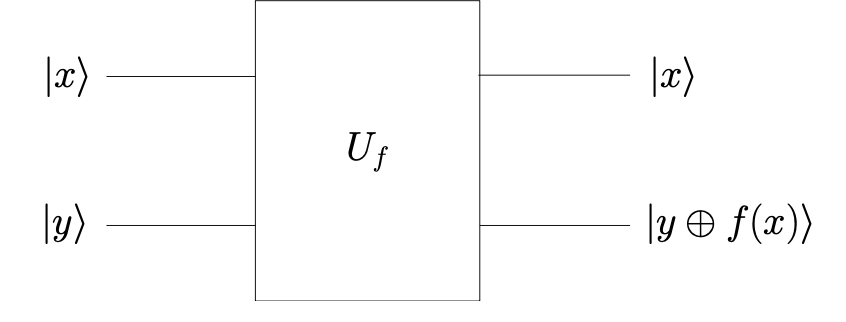
\includegraphics[width=0.5\textwidth]{Figs/FunctionOracle.png}
    \caption{Quantum circuit of a unitary operator mapping \(\ket{x}\ket{y} \rightarrow \ket{x}\ket{y\oplus f(x)}\) for any \(x, y \in \{0, 1\}\) (i.e. \(\ket{x}, \ket{y}\) denote standard basis states)}
    \label{fig:Uf}
\end{figure}

Observe now that \(U_f\) is reversible — this is because running \(U_f\) again on its output returns the original state \(\ket{x}\ket{y}\). Also note that we have not specified the inner workings of \(U_f\) but will rather treat \(U_f\) as a “black box” or “oracle” which we presume we can run, but cannot “look inside” to see its implementation details.

Of course, there is an easy way to determine whether f is constant or balanced — simply evaluate f on inputs 0 and 1, i.e. compute f(0) and f(1), and then check if f(0) = f(1). This naive (classical) solution, however, requires two queries or calls to \(U_f\) (i.e. one to compute \(f(0)\) and one to compute \(f(1)\)). So certainly at most two queries to Uf suffice to solve this problem. Can we do it with just one query? Classically, the answer turns out to be no. But quantumly, Deutsch showed how to indeed achieve this with a single query.

\begin{figure}[h]
    \centering
    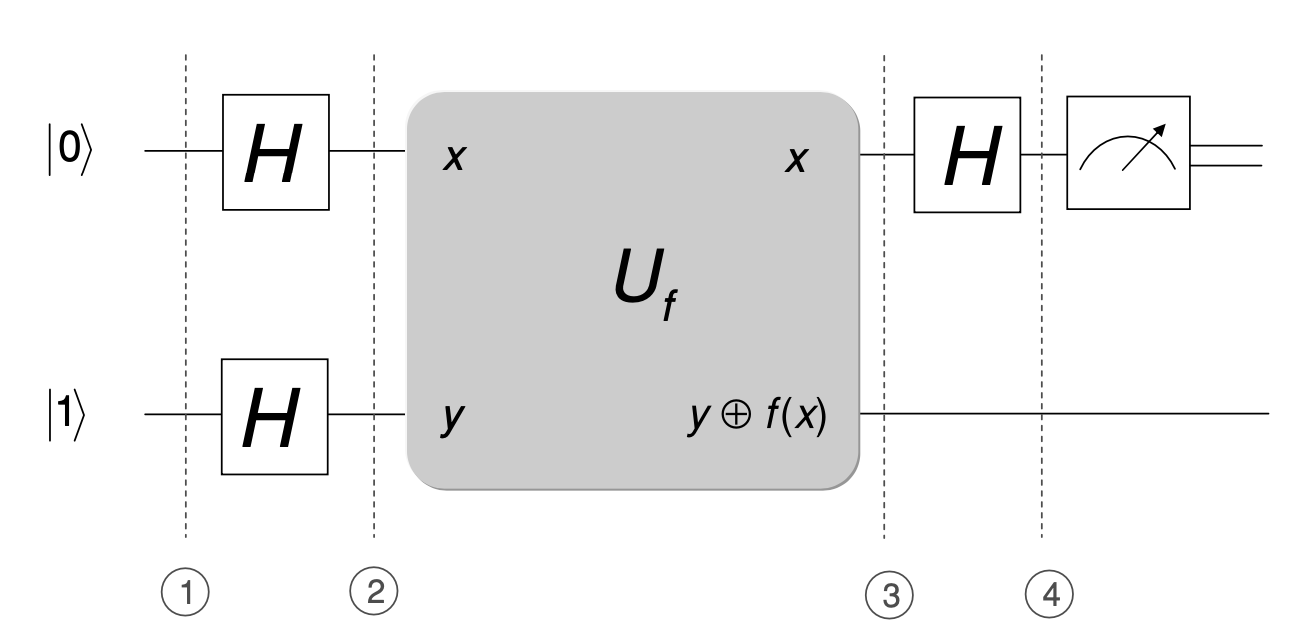
\includegraphics[width=0.7\textwidth]{Figs/DeutschCircuit.png}
    \caption{The Deutsch Algorithm}
    \label{fig:Deutsch}
\end{figure}

Let us walk through the steps: 
\begin{align*}
    \ket{\psi_1} &= \ket{0}\ket{1} \\
    \ket{\psi_2} &= \ket{+}\ket{-} = \frac{1}{\sqrt{2^2}}(\ket{0} + \ket{1})(\ket{0} - \ket{1}) = \frac{1}{\sqrt{2^2}}(\ket{0}(\ket{0} - \ket{1}) + \ket{1}(\ket{0} - \ket{1}))\\
    \ket{\psi_3} &= \frac{1}{\sqrt{2^2}}(\: \ket{0}(\ket{0\oplus f(0)} - \ket{1\oplus f(0)}) + \ket{1}(\ket{0\oplus f(1)} - \ket{1\oplus f(1)}) \:) \\
           &= \frac{1}{\sqrt{2^2}}(\:\ket{0}(-1)^{f(0)}(\ket{0} - \ket{1}) + \ket{1}(-1)^{f(1)}(\ket{0} - \ket{1})\:) \\
           &= \frac{1}{\sqrt{2}}(\:\ket{0}(-1)^{f(0)} + \ket{1}(-1)^{f(1)}\:) \ket{-} \\    
\end{align*}
At this step, we can drop the second qubit and focus on the first qubit. Transform this qubit by a Hadamard matrix, we have
\begin{align*}
 \ket{\psi_4} &= \frac{1}{2} ((-1)^{f(0)} \ket{+} + (-1)^{f(1)} \ket{-}) \\
        &= \frac{1}{2} ( (-1)^{f(0)} +
(-1)^{f(1)})\ket{0} +  ((-1)^{f(0)} -
(-1)^{f(1)})\ket{1} ) \\  
\end{align*}
The measurement, by projecting onto the basis \(\{\ket{0}, \ket{1}\) will either be in classical state \(0\) when \(f(0) = f(1)\)  or \(1\) when \(f(0) \neq f(1).\) 
 
\subsection{The Deutsch-Jozsa Algorithm}
The Deutsch-Jozsa algorithm is the generalization of the Deutsch algorithm: it determines whether a function \(f: \{0,1\}^n \rightarrow \{0,1\}\) is constant or balanced if it is promised only these two are the only possibilities. 

It will be a great exercise to walk through the qubits in the Figure~\ref{fig:DeutschJozsa}. 

\begin{align*}
    \ket{\psi_0} &= \ket{0}^{\otimes n}\ket{1} \\
    \ket{\psi_1} &= \frac{1}{\sqrt{2^n}}\ket{+}^{\otimes n}\ket{-} \\
           &= \frac{1}{\sqrt{2^n}} \sum_{x=0}^{2^n-1} \ket{x}\ket{-} \\
    \ket{\psi_2} &= \frac{1}{\sqrt{2^{n+1}}}\sum_{x=0}^{2^n-1}\ket{x} (\ket{0\oplus f(x)} - \ket{1\oplus f(x)} \\
           &= \frac{1}{\sqrt{2^{n+1}}}\sum_{x=0}^{2^n-1}\ket{x}(-1)^{f(x)} (\ket{0} - \ket{1}) \\
           &= \frac{1}{\sqrt{2^{n}}}\sum_{x=0}^{2^n-1}\ket{x}(-1)^{f(x)} \ket{-} \\ 
\end{align*}

\begin{figure}[h]
    \centering
    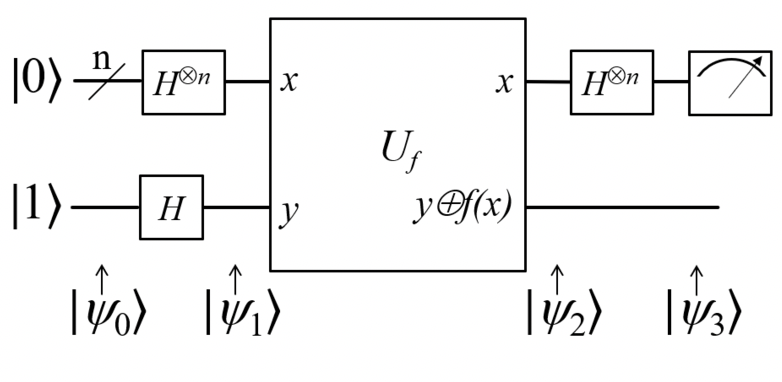
\includegraphics[width=0.7\textwidth]{Figs/Deutsch_algorithm.png}
    \caption{The Deutsch-Jozsa Algorithm}
    \label{fig:DeutschJozsa}
\end{figure}

At this stage, we can drop the last qubit and focus on the first \(n\) qubits. Transform them by a Hadamard matrix, by Lemma 6.2, we have
\begin{align*}
 \ket{\psi_3} &= \frac{1}{2^n} \sum_{x=0}^{2^n-1} \sum_{x} (-1)^{f(x)} \sum_z (-1)^{x\cdot z} \ket{z}  \\  
 &= \frac{1}{2^n} \sum_z  \ket{z} \sum_{x} (-1)^{f(x) + x \cdot z} \\
\end{align*}

If we focus on the \(\ket{z=0}\) state, its coefficient is  \(\frac{1}{2^n}(\sum_{x} (-1)^{f(x)})\), which is either \(1\) if \(f(x)\) is constant or \(0\) if \(f(x)\) is balanced. In the first case, this must be the only quantum state the system is in as the quantum state has coefficient. Projecting onto this state thus gives us the computational desired result whether the function is balanced or constant.  

\section{Exercise}
p1. Calculate the output quantum state of the following circuit if the input \(x_1 = \ket{0}, x_2 = \ket{0}\).

\begin{figure}[h]
    \centering
    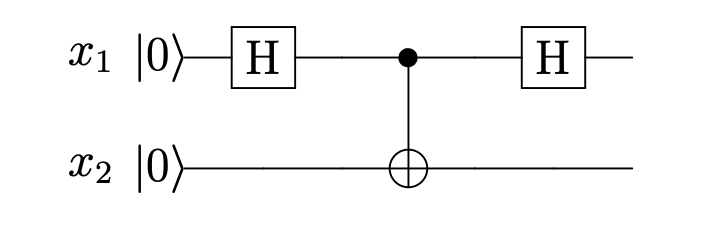
\includegraphics[width=0.5\textwidth]{Figs/QI_p1.png}
    \caption{Quantum circuit to analyze}
    \label{fig:QIex1}
\end{figure}


p2. A SWAP gate takes two inputs \(x_1\) and \(x_2\) and outputs \(x_2\) and \(x_1\); i.e., it swaps the values of two registers. Show how to build a SWAP gate using only CNOT gates. (Hint: you’ll need \(3\) of them.)
\newpage

\Lecturer{Hui Jin}
\Contributor{}
\LectureNumber{14}
\LectureDate{DATE}
\LectureTitle{Shor's Factoring Algorithm}

\lstset{style=mystyle}


	\MakeScribeTop

%#############################################################
%#############################################################
%#############################################################
%#############################################################

\section{Introduction}
Shor's factoring algorithm is one of the most important quantum algorithms ever discovered and is widely regarded as a landmark result in quantum computing. In principle, a sufficiently large fault-tolerant quantum computer running Shor's algorithm could break RSA, one of the most widely used public-key cryptosystems in modern Internet security. The possibility of large-scale quantum computers has motivated significant research into post-quantum cryptography, which aims to develop cryptographic systems resistant to quantum attacks. 

The RSA algorithm relies on a simple yet profound idea: prime factorization is a practically hard problem. Although an elementary school student understands the basic idea of factorization, the actual computation to factor a large number involves an insurmountable computation, at least for all known algorithms on a classical computer. 

Here is the problem statement: given a number \(N\), and the knowledge that \(N\) is a product of two prime numbers \(p, q\), how do we find these two primes? 

The best known classical factoring algorithms require super-polynomial time in the number of bits of N. 

Shor's factoring algorithm running on a quantum computer has complexity: 
\begin{align*}
    \mbox{Quantum Complexity}_N = O((\log N)^3),
\end{align*}
which is polynomial complexity. Therefore quantum algorithm achieves an exponential speedup over classical algorithms. 

\section{Shor's factoring algorithm overview}
At its core, Shor's prime factorization algorithm is a sub-quantum routine that finds the order of an integer in the ring \(Z_N\). 

\begin{lemma}
Given \(N\), which is odd and not a power of a prime, and an integer \(a < N\), where  \(GCD(a, N) = 1\). The order \(r\) of \(a\) is defined as the minimum  \(r\) such that
\begin{align*}
    a^{r} \equiv 1 \pmod{N}
\end{align*}
\end{lemma}

Knowing the order, the other parts of Shor's factoring algorithm rely on classical computers, with polynomial complex. Here is the overview of Shor's factoring algorithm.


So the key step is the order finding algorithm, which can be solved in polynomial time on a quantum computer. The quantum algorithm relies on the quantum phase estimation. By before we can describe the phase estimation quantum algorithm, we first need to describe quantum Fourier transform.



\section{Quantum Fourier Transform}
A classical discrete Fourier Transform (DFT) linearly maps a vector of length \(N\) \(x = (x_0, x_1, \cdots x_{N-1})\) to another vector length \(N\) \(y=(y_0, y_1, \cdots, y_{N-1})\) by the following transformation: 
\begin{align*}
    y_j = \sum_{k=0}^{N-1} \omega_{N}^{kj} x_k,
\end{align*}
for \(j=0, 1, \cdots, N-1\), where \(\omega_{N} = e^{2\pi i/N}. \)

Similarly, the quantum Fourier Transform has the same form, where it maps the (superposition) state of \(n=\log_2 N\) qubits
\begin{align}
    \ket{x} = \sum_{i=0}^{N-1} x_i \ket{i}
\end{align}

to another state of \(n\) qubits:
\begin{align}
    \ket{y} = \sum_{i=0}^{N-1} y_i \ket{i}
\end{align}
by the following transformation: 
\begin{align*}
    y_j = \frac{1}{\sqrt{N}} \sum_{k=0}^{N-1} \omega_{N}^{kj} x_k,
\end{align*}
for \(j=1, \cdots, N\), where \(\omega = e^{2\pi i/N}. \) Note that to make the transformation a unitary operation, we introduced a normalization factor \(\frac{1}{\sqrt{N}}\) compared to conventional discrete Fourier transform. 

As quantum circuit has linear property, we can focus on the input of quantum Fourier Transform being basis state \(\ket{x}\), where \(x\) is an integer between \(0\) and \(N-1\), then each \(y_j\) equals to \(\omega_N^{xj}\). Like \(\ket{x}\) where we abuse the notion a bit by assuming it is the base state now, let us use \(\ket{y}\) to denote \(j\). Then the quantum Fourier transform can be equivalently described as a linear mapping between base states \(\ket{x}\) and \(\ket{y}\):
\begin{align}
    \mbox{QFT: } \ket{x} \rightarrow \frac{1}{\sqrt{N}} \sum_{y=0}^{N-1} \omega_{N}^{xy} \; \ket{y}.
    \label{eq:baseState}
\end{align}
Similar to Hadamard transform, a QFT maps a basis state to a superposition of base states with a distinct structure. In fact it is informative to compare the Hadamard transform mapping:
\begin{align*}
    H_N: \ket{x} \rightarrow \frac{1}{\sqrt{N}} \sum_{y=0}^{N-1} (-1)^{x \cdot y} \; \ket{y},
\end{align*}
where \(x\cdot y\) is an inner product of the \(x, y\) binary representation vector.

As we know the mapping of the basis state \(\ket{x}\) picks up the \(x\) column of the unitary matrix, Eq.~\ref{eq:baseState} reveals that the unitary matrix (or quantum gates) for the QFT is: 
\begin{align}
\frac{1}{\sqrt{N}}
\begin{pmatrix}
1 & 1 & 1 & \cdots & 1 \\
1 & \omega_N & \omega_N^2 & \cdots & \omega_N^{N-1} \\
1 & \omega_N^2 & \omega_N^4 & \cdots & \omega_N^{2(N-1)} \\
\vdots & \vdots & \vdots & \ddots & \vdots \\
1 & \omega_N^{N-1} & \omega_N^{2(N-1)} & \cdots & \omega_N^{(N-1)^2}
\end{pmatrix}.    
\label{eq:QFT}
\end{align}

\begin{example} \(1\) qubit ((N=2))
Since \(\omega_2=e^{\pi i}=-1\),
\[\mbox{QFT}_2 = 
\frac{1}{\sqrt{2}}
\begin{pmatrix}
1 & 1\\
1 & -1
\end{pmatrix}.
\]
This is exactly the Hadamard gate.
\end{example}


\begin{example}
2 qubits ((N=4)).

Here \(\omega_4=i\), so
\[ \mbox{QFT}_4 = 
\frac{1}{2}
\begin{pmatrix}
1 & 1 & 1 & 1\\
1 & i & -1 & -i\\
1 & -1 & 1 & -1\\
1 & -i & -1 & i
\end{pmatrix}.
\]
\end{example}


\subsection{Implementation of Quantum Fourier Transform}
The quantum circuit corresponding to the unitary matrix Eq.~\ref{eq:QFT} is known as the QFT quantum circuit. The structure can be defined in a recursive manner. The core technique involved is reminiscent of the Fast Fourier Transform. 

Let's look at the mapping Eq~\ref{eq:baseState}. We claim that it can be decomposed as a tensor product of \(n\) qubits, just like Hadamard transform. Unlike Hadamard transform, where each qubit is a \(\ket{+}\) or \(\ket{-}\) in the Tensor product, here each qubit is in the form of \(\ket{0} + e^{2\pi i \; 0.x_{k-1}\cdots x_0} \ket{1}\), where \(0.x_{k-1}\cdots x_0 = 2^{-1}x_{k-1} + 2^{-2}x_{k-2}+ \cdots + 2^{-k}x_0.\)

In fact, we rewrite Eq~\ref{eq:baseState} as: 
\begin{align*}
    \mbox{QFT } \ket{x} &= \frac{1}{\sqrt{2^n}} \sum_{y=0}^{2^n-1} \omega_{2^n}^{xy} \; \ket{y} \\
    &= \frac{1}{\sqrt{2^n}} \sum_{y=0}^{2^n-1} e^{2\pi i \frac{xy}{2^n}} \; \ket{y} \\
    &= \frac{1}{\sqrt{2^n}} \sum_{y_0=0}^{1}\sum_{y_1=0}^{1}\cdots\sum_{y_{n-1}=0}^{1}  e^{2\pi i \frac{x(2^{n-1} y_{n-1} +2^{n-2} y_{n-2} + \cdots + y_0)}{2^n}} \; \ket{y_{n-1}y_{n-2}\cdots y_0} \\
    &= \frac{1}{\sqrt{2^n}} 
    (\ket{0} + e^{2\pi i x \frac{1}{2}}\ket{1})\otimes
    (\ket{0} + e^{2\pi i x \frac{1}{4}}\ket{1}) \otimes
    \cdots 
    (\ket{0} + e^{2\pi i x \frac{1}{2^{n-1}}}\ket{1}) \\
    &= \frac{1}{\sqrt{2^n}} 
    (\ket{0} + e^{2\pi i \; 0.x_0}\ket{1})\otimes
    (\ket{0} + e^{2\pi i \;0.x_1x_0}\ket{1}) \otimes
    \cdots 
    (\ket{0} + e^{2\pi i \;0.x_{n-1}x_{n-2}\cdots x_0}\ket{1}). 
\end{align*}
Here \((\ket{0} + e^{2\pi i \; 0.x_0}\ket{1})\) corresponds to the \(n\)-th qubit \(\ket{y_{n-1}}\), \((\ket{0} + e^{2\pi i \; 0.x_1x_0}\ket{1})\) corresponds to the \((n-1)\)-th qubit \(\ket{y_{n-2}}\), and so on. So the mapping involves a reverse ordering. 

The implementation now uses a controlled phase shift quantum gate (CP). 


A normal phase shift quantum gate has the following property: 
\[\mbox{Phase Shift}: \ket{0} + \ket{1} \rightarrow \ket{0}+ e^{i \theta} \ket{1}.\]


In contrast, a controlled-phase shift quantum gate introduces a control qubit, with the following unitary matrix: 
\[ \mbox{CP} = 
\begin{pmatrix}
1 & 0 & 0 & 0\\
0 & 1 & 0 & 0\\
0 & 0 & 1 & 0\\
0 & 0 & 0 & e^{i\theta}
\end{pmatrix}.
\]
Here is the mapping of the basis states for a controlled-phase shift of \(\theta\): 
\begin{align*}
  \mbox{CP}\ket{00} &= \ket{00} \\
  \mbox{CP}\ket{01} &= \ket{01} \\
  \mbox{CP}\ket{10} &= \ket{10} \\
  \mbox{CP}\ket{11} &= e^{i \theta} \ket{11} 
\end{align*}

Let's see how we implement the qubits in 
\[
\frac{1}{\sqrt{2^n}} 
    (\ket{0} + e^{2\pi i \; 0.x_0}\ket{1})\otimes
    (\ket{0} + e^{2\pi i \;0.x_1x_0}\ket{1}) \otimes
    \cdots 
    (\ket{0} + e^{2\pi i \;0.x_{n-1}x_{n-2}\cdots x_0}\ket{1}). 
\]
Assume we order the qubits as \(\ket{x_{n-1}}, \ket{x_{n-2}} \cdots \ket{x_0}\), where \(\ket{x_{n-1}}\) is on the top branch and \(\ket{x_0}\) is at bottom, then we can obtain \(\ket{y_0} = \ket{0} + e^{2\pi i \;0.x_{n-1}x_{n-2}\cdots x_0}\ket{1}\) on the top branch by implementing a Hadamard transform on \(\ket{x_{n-1}}\), followed by a \(\ket{x_{n-2}}\) controlled phase shift of \(e^{2\pi i/4}\), followed by a \(\ket{x_{n-3}}\) controlled phase shift of \(e^{2\pi i/8}\), and so on, the last one \(\ket{x_{0}}\) controlled phase shift of \(e^{2\pi i/2^{n}}\). A similar circuit generates the \(k-th\) qubit \(\ket{y_{k-1}}\). In order to have the qubits ordered from \(\ket{y_{n-1}}, \ket{y_{n-2}}, \cdots, \ket{y_0}\), we do pair-wise swapping: swap the top and bottom qubits, the second top and second bottom, and so on. 

\begin{figure}[h]
    \centering
    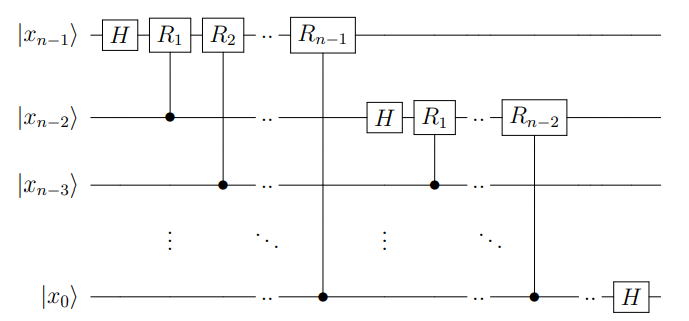
\includegraphics[width=0.85\textwidth]{Figs/QFT.png}
    \caption{Quantum Fourier Transform. Here \(R_k\) represents controlled-phase shift gate with phase \(2\pi /2^{k+1}\). Qubits here are indexed from \(0\) to \(n-1\).}
    \label{fig:PEA}
\end{figure}


\section{Phase Estimation Problem}
The quantum phase estimation problem, 
\begin{lemma}
Given a quantum circuit \(U\) and an eigenvector \(\ket{\psi}\) that satisfies:
\begin{align*}
    U \ket{\psi} = e^{2\pi i \theta} \ket{\psi}  
\end{align*}
we have an efficient way to approximate \(\theta\). The approximation \(\theta \approx \frac{y}{2^m}\) has error less than \(\frac{1}{2^m}\), where \(m\) is the number of qubits used for this approximation.      
\end{lemma}

Here we assume \(\ket{\psi}\) is provided and promised to be an eigenvector. It means that we have \(\ket{\psi}\) as the input to a quantum circuit. 

A basic diagram for the quantum phase estimation is depicted in Figure~\ref{fig:PEA}, for \(m=3\). One of the critical module used is the \(QFT^{-1}\), the inverse quantum Fourier Transform. We shall first describe it in the next section before we come back to the details of quantum phase estimation.
\begin{figure}[h]
    \centering
    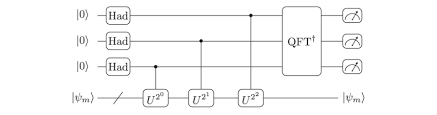
\includegraphics[width=0.85\textwidth]{Figs/PEA.png}
    \caption{Quantum Phase Estimation Circuit for \(m=3\). Estimation precision can be increased by increasing \(m\), along with complexity.}
    \label{fig:PEA}
\end{figure}

The key principle here is the phase kick-back mechanism. 
For example, a single control qubit running a controlled-\(U^{2^k}\) acts globally as:
\begin{align*}
CU^{2^k} \ket{0}\ket{\psi} &\rightarrow \ket{0}{\psi} \\
CU^{2^k} \ket{1}\ket{\psi} &\rightarrow e^{2\pi i (2^k \theta)} \ket{1}\ket{\psi} \\ CU^{2^k} (\ket{0}+\ket{1})\ket{\psi} &\rightarrow (\ket{0}+e^{2\pi i (2^k \theta)}\ket{1})\ket{\psi} 
\end{align*}
We see that the controlled-\(U^{2^k}\) gate injects a phase shift into the controlled qubit. 

Therefore, we can write down the system state after each controlled-\(U^{2^k}\) operation. Before the first controlled operation, the state is 
\begin{align*}
    \ket{+}\ket{+}\ket{+}\ket{\psi_m}
\end{align*}
After the first controlled operation \(U^{2^0}\) by the third qubit, the quantum state is:
\begin{align*}
    \ket{+}\ket{+}(\ket{0} + e^{2\pi i\theta}\ket{1})\ket{\psi_m}
\end{align*}
After the second controlled operation \(U^{2^1}\) by the second qubit, the quantum state is:
\begin{align*}
    \ket{+}(\ket{0} + e^{2\pi i 2\theta}\ket{1})(\ket{0} + e^{2\pi i\theta}\ket{1})\ket{\psi_m}
\end{align*}

Finally after the third controlled operation \(U^{2^2}\) by the first qubit, the quantum state is:
\begin{align*}
    (\ket{0} + e^{2\pi i 4\theta}\ket{1})(\ket{0} + e^{2\pi i 2\theta}\ket{1})(\ket{0} + e^{2\pi i\theta}\ket{1})\ket{\psi_m}
\end{align*}
Looking at the first qubits closely, we realize that this is exactly (up to a constant scaling \(\frac{1}{\sqrt{2^n}}\)), the quantum Fourier transform of base state \(\ket{y}\), where \(\theta\) is approximated by an m-bit integer \(y\), in other words \(\theta \approx y/2^m\). Therefore, the inverse Fourier transform recovers the basis state \(\ket{y}\)!

The above algorithm is exact and deterministic if \(\theta = \frac{y}{2^m}\). When \(\frac{y-1}{2^m} < \theta < \frac{y}{2^m}\), then the measure of the \(m\)-th qubit is probabilistic. By increasing \(m\), we improve the approximation accuracy.

\section{Quantum Order Detection}
The quantum phase estimation algorithm facilitates an efficient solution of a classically difficult number theory problem - finding the order of a number \(a\) in \(Z_N\). For integer \(1\leq a < N\), the order of \(a\) of modulus \(N\) is defined as the minimum number \(r\) such that 
\begin{align*}
    a^r \equiv 1 \pmod {N}
\end{align*}

\subsection{Unitary operation and its Eigenvectors}
We define the mapping \(U_a\) as:
\begin{align*}
    U_a \ket{k} = \ket{ak}  \pmod{N}, 
\end{align*}
for \(k=0, 1, \cdots, N-1.\)
Since \(U_a\) corresponds to a permutation matrix, it is unitary and must corresponds to a quantum circuit. 

Let's try to find the eigenvectors and their corresponding eigenvalues of this unitary matrix. 

Consider 
\begin{align*}
    \ket{\psi_j} = \frac{1}{\sqrt{r}} \sum_{k=0}^{r-1} \omega_r^{-jk}\ket{a^k},
\end{align*}
where \(\omega_r = e^{2\pi i \frac{1}{r}}.\)

If we apply \(U_a\) on qubits \(\ket{\psi_j}\), we have 
\begin{align*}
    U_a \ket{\psi_j} &= \frac{1}{\sqrt{r}} \sum_{k=0}^{r-1} \omega_r^{-jk}\ket{a^{k+1}}\\
    &= \omega_r^{j} \frac{1}{\sqrt{r}} \sum_{k=0}^{r-1} \omega_r^{-jk}\ket{a^k} \\
    &= \omega_r^{j} \ket{\psi_j}.
\end{align*}
That means \(\ket{\psi_j}\) is an eigenvector with eigenvalue \(\omega_r^{j} = e^{2\pi i \frac{j}{r}}\).

If the eigenvector is prepared properly, we can use the phase estimation algorithm to extract the phase \(\frac{j}{r}\) by approximating it to a number \(\frac{y}{2^m}\). If \(m\) is sufficiently large, \(\frac{j}{r}\) can be extracted exactly from \(\frac{y}{2^m}\).


\subsection{Continued Fraction Extraction}

The quantum measurement step yields an estimate $\phi \approx \frac{j}{r}$ formatted as a dyadic fraction $\frac{y}{2^m}$. To extract the true period $r$ from this measured value, we use the classical **Continued Fractions Algorithm**.

The continued fraction expansion expresses the measured ratio $\frac{y}{2^m}$ as a nested fraction:
\begin{align*}
    \frac{y}{2^m} = a_0 + \cfrac{1}{a_1 + \cfrac{1}{a_2 + \cfrac{1}{a_3 + \dots}}}
\end{align*}
Truncating this expansion at successive depths produces a sequence of rational approximations $\frac{p_k}{q_k}$ known as *convergents*. By choosing a register size $m \geq 2\log_2 N + 1$, bounded error properties guarantee that the true fraction $\frac{j}{r}$ appears explicitly as one of these unique convergents $\frac{p_k}{q_k}$.

The classical post-processing steps are executed as follows:
\begin{enumerate}
    \item Compute the sequence of convergents $\frac{p_k}{q_k}$ for the measured fraction $\frac{y}{2^m}$.
    \item For each convergent with a denominator $q_k < N$, test whether $q_k$ serves as the valid period by checking if $a^{q_k} \equiv 1 \pmod{N}$.
    \item If the condition holds, set $r = q_k$. If $j$ and $r$ share a common factor, the convergent will reduce to a simplified form $\frac{p_k}{q_k} = \frac{j/d}{r/d}$. In this scenario, the test fails, and the algorithm is restarted. Over multiple runs, the probability of sampling a coprime value for $j$ is sufficiently high to guarantee finding the correct period $r$ in $O(1)$ repetitions.
\end{enumerate}

\section{Period finding: A problem at the heart of quantum computing}
While trends may have moved on, the idea of extracting group structure from the Fourier spectrum is still at the very core of what quantum computers could be useful for. Scott Aaronson, for example, in his 2022 commentary “How Much Structure Is Needed for Huge Quantum Speedup?” presents the following hierarchy:

 \begin{figure}[h]
    \centering
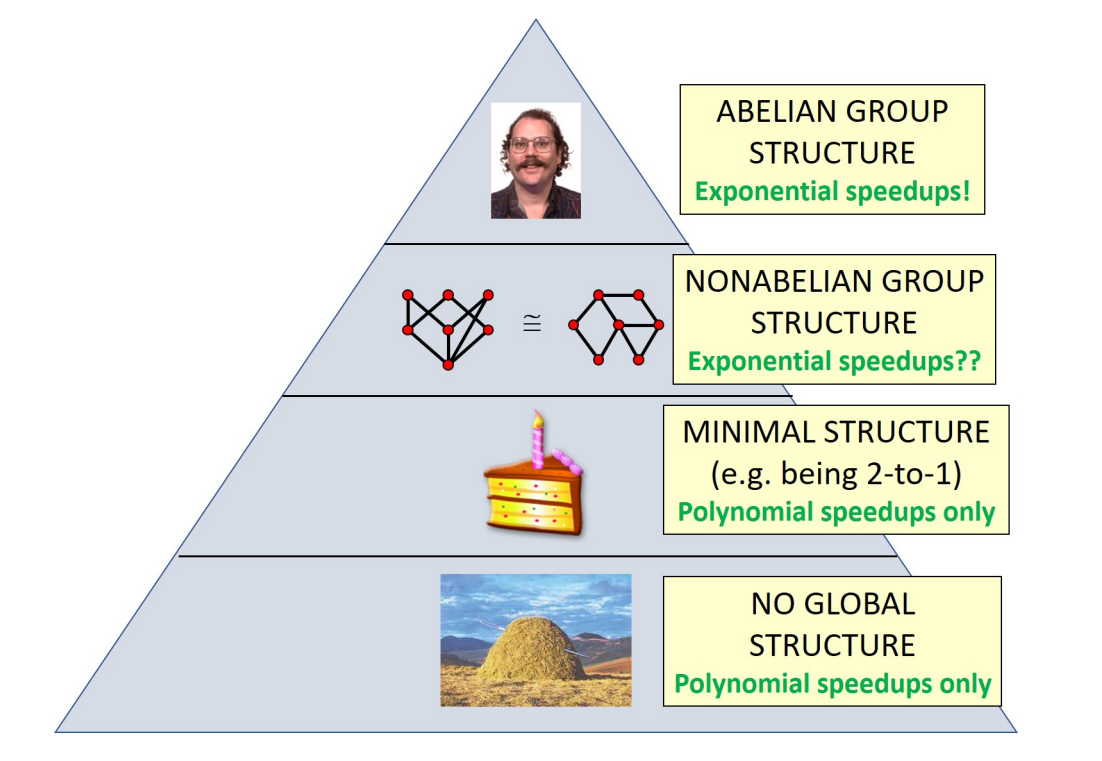
\includegraphics[width=0.6\textwidth]{Figs/aaronson_fig6.png}
    \caption{Speedup.}
    \label{fig:QFT}
\end{figure}




















    

\newpage

%\Lecturer{Hui Jin}
\Contributor{}
\LectureNumber{14}
\LectureDate{DATE}
\LectureTitle{Quantum Error Correction Codes}

\lstset{style=mystyle}


	\MakeScribeTop

%#############################################################
%#############################################################
%#############################################################
%#############################################################

\section{Introduction}
Despite the great promise held by the quantum computing, quantum noise poses a major challenge in the development of quantum computers as it can cause qubits to lose their delicate quantum state, known as decoherence.

Quantum Noise refers to the unwanted disturbances that affect quantum systems, leading to errors in quantum computations. Unlike classical noise, which might simply add random errors to a signal, quantum noise can have more complex and detrimental effects. 

Quantum noise can arise from various sources, including thermal fluctuations, electromagnetic interference, imperfections in quantum gates, and interactions with the environment. Different types of quantum noise affect qubits in distinct ways. For example, phase noise alters the relative phase between the basis states of a qubit, while amplitude noise affects the probabilities of measuring different states. 

Quantum noise creates a significant barrier to the development of large-scale, fault-tolerant quantum computers. Even small amounts of noise can lead to decoherence, causing qubits to lose their superposition and entanglement properties. This loss of quantum information can render computations meaningless and limit the size and complexity of feasible quantum algorithms. 


Efforts to mitigate quantum noise include improving the physical isolation of qubits, developing more precise control techniques. The most promising technique among them is quantum error correction codes, which is our focus here. 


Quantum error correction (QEC) is used in quantum computing to protect quantum information from errors due to decoherence and other quantum noise. Quantum error correction is essential to achieve fault tolerant quantum computing that can reduce the effects of noise on stored quantum information, faulty quantum gates, faulty quantum preparation, and faulty measurements. This would allow algorithms of greater circuit depth and allow us build large scale quantum computers.

Error correction itself is not a new concept; classical error correction codes started around the year of 1948, when Shannon invented the channel coding theory and Hamming independently created the first non-trivial code Hamming code. Quantum error correction (QEC) requires much more thought. On a fundamental level, standard classical error correction only needs to correct bit flip errors, where bits accidentally switch from \(0\) to \(1\) or vice versa. Such error are digitized and big. Quantum computers must correct more kinds of errors, like phase errors which can corrupt the extra quantum information that qubits carry and does not have a counterpart in the classical world. Not only that, but QEC techniques must correct errors without the ability to copy unknown quantum states, and without destroying the underlying quantum state.

In particular, the no-cloning theorem was a huge barrier to introduce the techniques in classical error correcting codes into the quantum world. The essence of classical error correction codes rests on the notion of duplication, or repetition. From the simplest repetition codes, to the state-of-the art low-density parity-check nodes, irregular repeat accumulate codes, repetition is an indispensable component of the code construction for structured redundancy. Since the no-cloning theorem say duplicating the qubit \(\ket{\phi}\) is not possible, how can we add redundancy? Miraculously, the quantum entanglement provides a solution.
 
 Another thorny obstacle in quantum error correcting codes is related to measurement.   If an error does occur on our encoded state, the natural thing to do is to perform a measurement on the state in order to diagnose the error. For example, the majority vote decoding algorithm for the repetition code relies on this simple concept. However, in the quantum world, measurements collapses the state and destroys the information we were trying to protect. To handle this problem, we use syndrome decoding where only error patterns are measured. Without measuring the data we do not collapse the quantum states. 

Let’s summarize the essential ideas that underlie the quantum error correction scheme:
\begin{itemize}
    \item The errors are digitized. Although the errors in the quantum information
were small, we performed measurements that projected our state onto either a state with no error, or a state with one of a discrete set of errors that we knew how to convert.

\item The errors are measured without measuring the data. Our measurements revealed the nature of the errors without revealing (and hence disturbing) the encoded information.

\item The errors are local, and the encoded information is nonlocal. It is important to emphasize the central assumption underlying the construction of the code – that errors affecting different qubits are, to a good approximation, uncorrelated. We have tacitly assumed that an event that causes errors in two qubits is much less likely than an event causing an error in a single qubit. It is of course a physics question whether this assumption is justified or not – we can easily envision processes that will cause errors in two qubits at once. If such correlated errors are common, coding will fail to improve reliability.
\end{itemize}

\section{No Cloning Theorem}
No cloning theorem says nature prevents us duplicating a general qubit.  
\begin{theorem}
In general we cannot clone a qubit unless it is a pure state.    
\end{theorem}

\begin{proof}
Let us assume that there exists an operation \(U_{cl}\) that we can apply to clone any qubit \(\ket{\phi} = \alpha \ket{0} + \beta \ket{1}\) to a pure state \(\ket{0}\), for arbitrary complex numbers \(\alpha, \beta\). That means we have 
\[U_{cl}(\ket{\phi}\ket{0}) = \ket{\phi}\ket{\phi},\]
for any qubit \(\ket{\phi}\).

If we expand the qubit \(\phi\) after the cloning, we have 
\begin{align*}
    U_{cl}(\ket{\phi} \ket{0}) &= \ket{\phi}\ket{\phi} \\
           &= (\alpha \ket{0} + \beta \ket{1})(\alpha \ket{0} + \beta \ket{1}) \\
           &= \alpha^2 \ket{00} + \alpha\beta\ket{01} + \alpha\beta\ket{10} + \beta^2 \ket{11}
\end{align*}

However, if we expand qubit \(\ket{\phi}\) first, and apply the cloning on the pure state, due to the linearity of quantum operation, we have 
\begin{align*}
   U_{cl} (\ket{\phi} \ket{0})  &= U_{cl}((\alpha \ket{0} + \beta \ket{1}) \ket{0}) \\
           &= \alpha U_{cl}(\ket{0}\ket{0}) +  \beta U_{cl}(\ket{1}\ket{0}) \\
           &= \alpha \ket{00} + \beta \ket{11}
\end{align*}
which does not have the cross states \(\ket{01}\) \(\ket{10}\). This is a contradiction unless \(\alpha\) or \(\beta\) equals to zero. 
\end{proof}

Since duplication, or repetition, is such a fundamental idea in error correcting code, the no-cloning theorem seemingly dealt a blow to the idea of quantum error correcting codes.

\section{Channel Noise Models}

\subsection{Bit-flip Noise}
The bit-flip noise converts the qubits 
\(\ket{0}\) and \(\ket{1}\) into each other. Hence, the original qubit \(\ket{q} = \alpha \ket{0} + \beta \ket{1}\) is distorted by the quantum noise into \(\ket{q} = \alpha \ket{1} + \beta \ket{0}\). We can think of the bit flip noise as transforming the original qubit by a Pauli matrix \(\sigma_X\).

This noise is similar to the binary symmetric channel in the classical world. 

Note that for the alternative basis states \(\ket{+}\), the bit-flip noise has no effect; for \(\ket{-}\), the bit=-flip noise changes the sign. 
In summary, we have:
\begin{align*}
    \sigma_X \ket{0} &= \ket{1} \\
    \sigma_X \ket{1} &= \ket{0} \\
    \sigma_X \ket{+} &= \ket{+} \\
    \sigma_X \ket{-} &= -\ket{-}
\end{align*}

\subsection {Phase Flip Noise}
A phase flip noise changes the phase of a qubit. For the base states, we have 
\(\ket{0} \rightarrow \ket{0}\), but \(\ket{1} \rightarrow - \ket{1}\).

Hence, the original qubit \(\ket{q} = \alpha \ket{0} + \beta \ket{1}\) is transformed by the quantum phase noise into \(\ket{q} = \alpha \ket{0} - \beta \ket{1}\); so the channel  introduces a dephasing factor \(e^{i\pi}\) between the two complex amplitudes \(\alpha, \beta\).

Note that for the alternative basis states \(\ket{+}\), the bit-flip noise changes it to \(\ket{-}\); for \(\ket{-}\), the bit-flip noise changes it to \(\ket{+}\). 


We can think of the phase flip noise as transforming the original qubit by a Pauli matrix \(\sigma_Z\).

This noise has no counterpart in classical world. 

In summary, we have:
\begin{align*}
    \sigma_Z \ket{0} &= \ket{0} \\
    \sigma_Z \ket{1} &= -\ket{1} \\
    \sigma_Z \ket{+} &= \ket{-} \\
    \sigma_Z \ket{-} &= \ket{+}
\end{align*}

With a clever trick, we can treat the phase-flip noise as bit-flip noise. In fact, we can verify that 
\begin{align*}
    \sigma_X = H \sigma_Z H \\
\end{align*}
By appending a Hadamard transformation before and after a channel noise \(\sigma_Z\), we have effectively a bit flip noise channel. This is illustrated in Figure~\ref{fig:QEC_BitFlipEquivalence}.

\begin{figure}[ht]
\centering
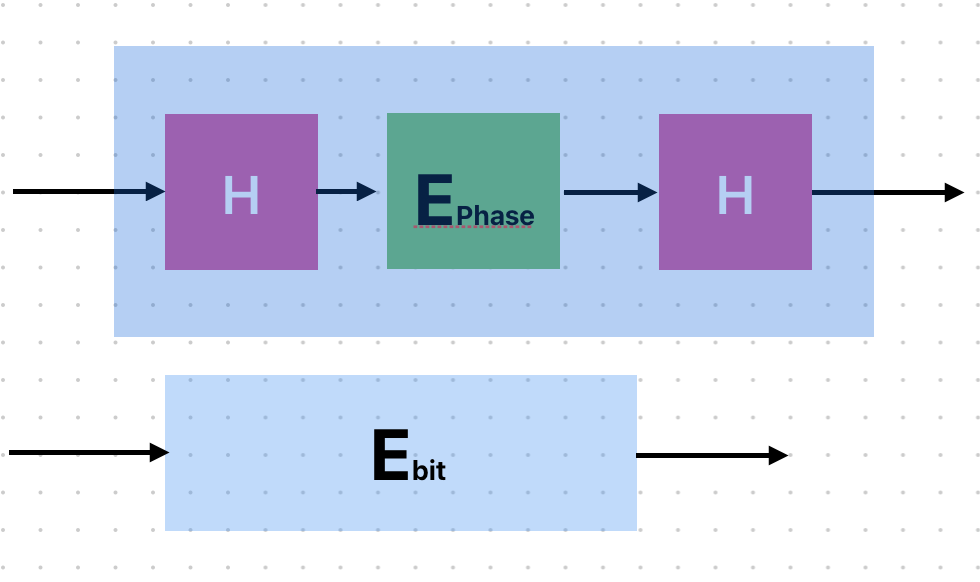
\includegraphics[width=0.7\textwidth]{Figs/BitFlip_equivalence.png}
    \caption{Channel phase-flip noise can be converted to bit-flip noise if we transform the qubit into the basis states \(\ket{+}\), \(\ket{-}\) by applying Hadamard transformation.}
\label{fig:QEC_BitFlipEquivalence}
\end{figure}


\subsection{Combination of bit-flip and phase-flip noise}
It is possible for qubits to experience both bit-flip and phase-flip noise simultaneously. Then the noise model of the channel is 
\[\sigma_X \sigma_Z \; \text{or} \; \sigma_Z \sigma_X\]

Let us against list the transformation by this noise on the two sets of basis states \(\{\ket{0}, \ket{1}\}\), and \(\{\ket{+}, \ket{-}\}\). There are eight cases:  
\begin{align*}
   \sigma_X \sigma_Z \ket{0} &= \ket{1} \\
   \sigma_Z \sigma_X \ket{0} &= -\ket{1} \\
   \sigma_X \sigma_Z \ket{1} &= \ket{0} \\
   \sigma_Z \sigma_X \ket{1} &= -\ket{0} \\
   \sigma_X \sigma_Z \ket{+} &= \ket{-} \\
   \sigma_Z \sigma_X \ket{+} &= -\ket{-} \\
   \sigma_X \sigma_Z \ket{-} &= \ket{+} \\
   \sigma_Z \sigma_X \ket{-} &= -\ket{+}
\end{align*}

\subsection{Other forms of Channel Noise}
Any type of channel noise on a single qubit, including small noises accumulated on the imperfect quantum gates, can be modeled by a unitary matrix multiplication. The unitary matrix of \(2\times 2\), can be decomposed to a linear combination of the four Pauli operators,
\begin{align*}
    E &= \begin{bmatrix}v_{00}&v_{01}\\v_{10}&v_{11}\end{bmatrix} \\
    &= \alpha_0 \begin{bmatrix}1 &0\\0&1\end{bmatrix} + \alpha_1 \begin{bmatrix}0 &1\\1&0\end{bmatrix} + \alpha_2 \begin{bmatrix}1 &0\\0&-1\end{bmatrix} + \alpha_3 \begin{bmatrix}0 &i\\-i&0\end{bmatrix} \\
    &= \alpha_i I + \alpha_1 \sigma_X + \alpha_2 \sigma_Z + \alpha_3 \sigma_Y
\end{align*}

So the (un-normalized) quantum state \(E\ket{\psi}\) can thus be written as a superposition of four terms, \(\ket{\psi}, \sigma_X\ket{\psi}, \sigma_Z\ket{\psi}, \sigma_X\sigma_Z\ket{\psi}\).


Any channel noise thus can be regarded as a tensor product of such linear combination of Pauli operators.  Note that \(\sigma_Y = -i \sigma_X \sigma_Z \). Therefore,  
if we can correct \(\sigma_X,\) and \(\sigma_Z\), we can correct any quantum error!

\subsection{The digitization of Quantum Noise}
Taking the set of qubits and the environment as a whole, then the evolution of the quantum state can be expressed in the form:
\begin{align}
\ket{\phi}\ket{\psi_{0}}_{e} \rightarrow \sum_i (E_i \ket{\phi}\ket{\psi_{i}}_{e} \label{eq:QuantumNoise}    
\end{align}
where each ‘error operator’ \(E_i\) is a tensor product of Pauli operators acting on the qubits, \(\ket{\phi}\) is the initial state of the qubits, and \(\ket{\psi_i}_e\)  are states of the environment. We thus express general noise and/or decoherence in terms of Pauli operators \(\sigma_X, \sigma_Y, \sigma_Z\) acting on the qubits. For clarity, we use denote \(X= \sigma_X, Z=\sigma_Z, Y=-i\sigma_Y = XZ\).

To write tensor products of Pauli matrices acting on \(n\) qubits, we introduce the notation \(X_uZ_v\) where \(u\) and \(v\) are \(n\)-bit binary vectors. The non-zero coordinates of \(u\) and \(v\) indicate where \(X\) and \(Z\) operators appear in the product. For example,

\begin{align}
    X \otimes I \otimes Z \otimes Y \otimes X = X_{10011} Z_{00110}.
\end{align}

Error correction is a process which takes a state such as \(E_i\ket{phi}\) to \(\ket{\phi}\). Correction of \(X\) errors takes \(Z_v\ket{phi}\)  to \(X_uZ_v\ket{phi}\); correction of \(Z\) errors takes \(X_uZ_v\ket{phi}\)  to \(X_u\ket{phi}\). Putting all this together, we discover the highly significant fact that to correct the most general possible noise, it is sufficient to correct just \(X\) and \(Z\) errors.


\section{Repetition Codes}
The first example of a Quantum error correction code is inspired by the repetition code in the classical world. 

\subsection{Review of the Classical Repetition Code}
If we send a single bit over a binary symmetric channel, one simple scheme offering protection is to encode the bit by repeating it multiple times, so that we can use the repetition at the receiver side. This is known as repetition codes. Assume we repeat three times, to transmit a \(0\) we send three bits (sequentially) in the state \(0\), and likewise for \(1\). We can say the encoder encodes the message bit as the following:
\begin{align*}
    0 &\rightarrow 000 \\
    1 &\rightarrow 111      
\end{align*}

Once the three bits have been received, after the noise, where each bit has probability \(p\) being flipped to the opposite bit, they are decoded by a “majority vote”. This intuitive decoding scheme guarantees that any single error is corrected. 

The majority vote decoding assumes measurement of the data bits, which is infeasible in quantum computation - measurement destroys quantum information. A different decoding method is to use syndrome decoding. We check parity by calculating the syndrome \((r_1+r_2, r_1+r_3)\), where \(r_i\) is the \(i\)-th received bit. In accordance of the syndrome, the decoder flips the corresponding bit: 
\begin{align*}
    00 &\rightarrow \text{No flip}   \\
    01 &\rightarrow \text{flip bit \(r_3\)} \\    
    10 &\rightarrow \text{flip bit \(r_2\)} \\  
    11 &\rightarrow \text{flip bit \(r_1\)}     
\end{align*}


For the decoding to fail (the decoder does not return the original transmitted bit), it must be true that either two of the three bits have been flipped (which can occur in three different ways), or all three have been flipped. So the decoding error probability is:
\[p'_{e} = 3 p^2 (1-p) + p^3,\]
which is less than \(p\) if \(p < 0.5\). Typically, \(p\) is small, and we can describe this as the error is reduced to \(O(p^2)\).

We would like to use the repetition idea in the quantum world. Even though the no-cloning theorem dictates that we cannot clone the qubits, we can use entanglement to effectively realize repetition. 

\subsection{The Three qubit code to correct one single bit-flip error}
The three-bit repetition code guarantees to return the correct bit value, so long as at most one of the bits in the code is flipped. We now use this as inspiration for the three-qubit code that can correct one single bit flip error. In the encoding, entanglement plays the role of the repetition. 

Figure~\ref{fig:QEC_BitFlip} shows the 1 logic qubit and 3 physical qubit quantum circuit that is enable to correct upto one single bit flip error. The figure shows three components: the encoder, the noise channel, and the decoder. The encoder entangle two ancillary qubit \(\ket{0}\) to the logic qubit so that for any input basis state \(\ket{b}\), the output is \(\ket{bbb}\),  based on two CNOT gates.

\begin{figure}[ht]
\centering
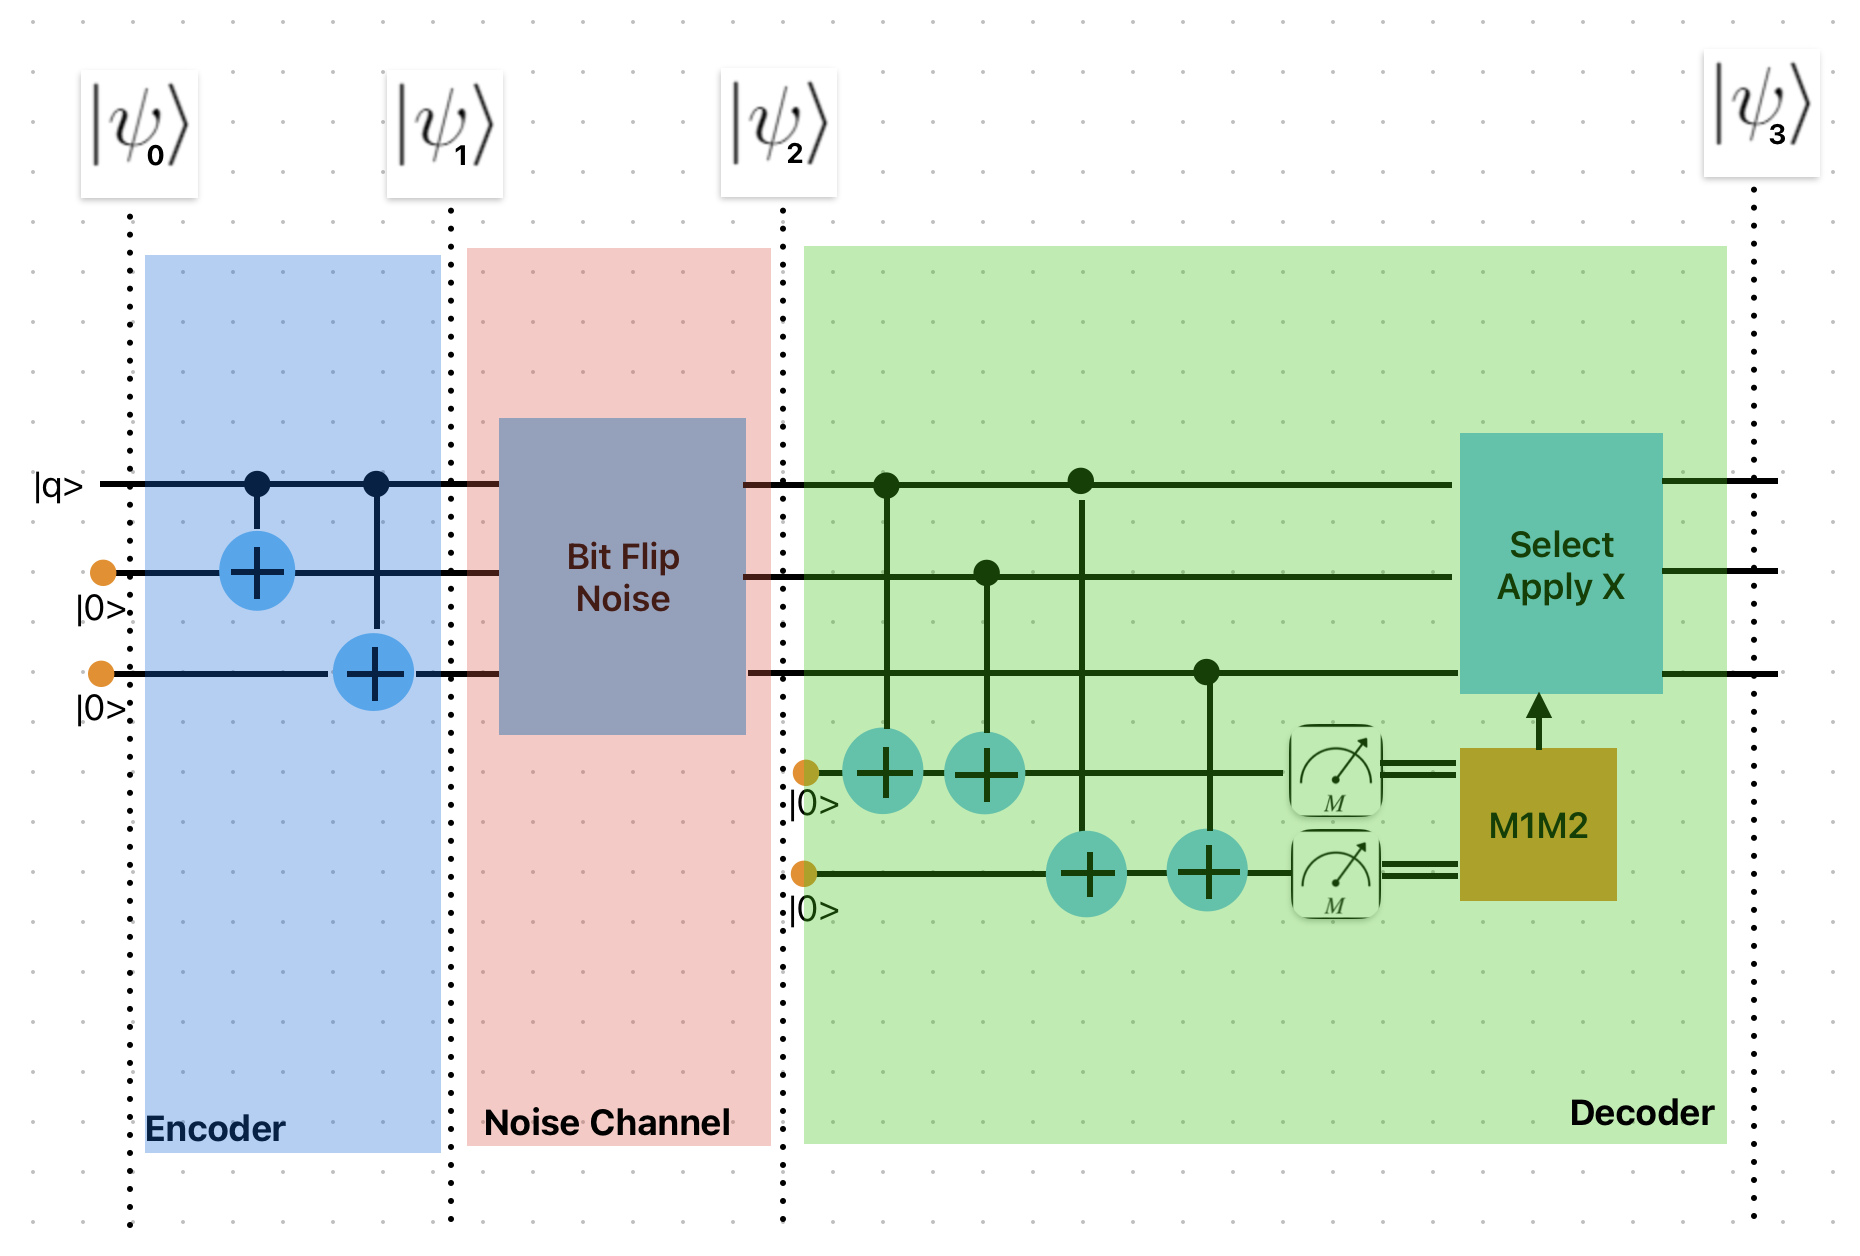
\includegraphics[width=0.98\textwidth]{Figs/QEC_BitFlipCorrect.png}
    \caption{Simple example illustrating the principles of quantum error correction. 
we want to transmit a single-qubit state \(\ket{\q} = \alpha \ket{0} + \beta\ket{1}\). The channel  introduces \(\sigma_X\) errors randomly. Encoder prepares two further qubits in the state \(\ket{0}\), represented by a small yellow circle, 
 and encodes the single qubit into a joint state of three qubits, by two controlled-not operations.
These three qubits go through the noisy channel. At the receiver end, the decoder recovers the joint state by extracting a
syndrome, and applying \(\sigma_X\) operation to one (or none) of the qubits based on the syndrome.}
    \label{fig:QEC_BitFlip}
\end{figure}


That is, we encode the computational basis states:
\begin{align*}
\ket{0} &\rightarrow \ket{\hat{0}} = \ket{000} \\
\ket{1} &\rightarrow \ket{\hat{1}} = \ket{111} 
\end{align*}

where \(\ket{\hat{0}}, \ket{\hat{0}}\) have the meaning of the logical \(\ket{0},\ket{1}\) qubits. Therefore for a general qubit \(a\ket{0} + \beta\ket{1}\), the output state is  
\[\alpha\ket{000} + \beta\ket{111} = \alpha \ket{0}^{\otimes3} + \beta \ket{1}^{\otimes3}.\]

Put together, the quantum encoder encodes the logic qubit \(a\ket{0} + \beta\ket{1}\) into three physical qubits through entanglement. In Figure~\ref{fig:QEC_BitFlip}, let us mark the joint qubits: 
\begin{align*}
\ket{\psi_0} &= (\alpha\ket{0}+\beta\ket{1})\ket{0}^{\otimes2}, \\ 
\ket{\psi_1} &=\alpha\ket{000}+\beta\ket{111}.    
\end{align*}

After passing through the bit-flip channel, the 3-qubit basis states \(\ket{000}, \ket{111}\) might have experienced zero, one, two, or, three qubit flips or errors. Just like classical repetition codes, at this stage, it seems we introduce more errors by doing entanglement. We will show, however, that now we can correct any single bit error and thus reduce the error rate. 

There are four output possibilities with the encoded qubits being distorted assuming at most one bit flip error:

\begin{table}[ht]
\caption{Outcome possibilities for a three qubits repetition code with at most one single error}
\begin{center}
\begin{tabular}{ |c |c | c | }
\hline
input & \text{Error Event} & Output (\(\ket{\psi_2}\))\\
\hline
\(\alpha\ket{000}+\beta\ket{111}\) & \text{no bit flipped} & \(\alpha \ket{000} + \beta \ket{111}\) \\
&\text{first qubit flipped} & \(\alpha \ket{100} + \beta \ket{011}\) \\
&\text{second qubit flipped}  & \(\alpha \ket{010} + \beta\ket{101}\) \\
&\text{third qubit flipped}  & \(\alpha \ket{001} + \beta \ket{110}\) \\
\hline
\end{tabular}
\end{center}
\end{table}


At the receiver end, receiving the corrupted \(3\)-qubit, the decoder now introduce two more qubits, prepared in the state \(\ket{00}
\). This extra pair of qubits, referred to as an ancilla, is not strictly necessary, but makes error correction easier to understand. The ancilla qubits are used to gather information about the noise. As discussed in the previous chapter, controlled-NOTs from the first and second received qubits to the first ancilla qubit computes the parity checks on the first two received qubits; controlled-NOTs from the first and third received qubits to the second ancilla bit computes the parity checks on the first and third received qubits. Measuring the two ancilla bits to the basis \(\{\ket{0} , \ket{1}\}\) gives two classical bits of information, we have a syndrome \(M_1, M_2\), completely analogous to the classical repetition codes. The error syndrome locates the error in the received qubits. Based on the syndrome, the decoder apply a Pauli swap matrix \(\sigma_X\) to one of the qubit to correct it. Suppose for example the decoder's syndrome is \(10\) (i.e. the ancilla state is projected onto \(\ket{10}\)). We see that the state of the received qubits must be  \(\alpha\ket{010} + \beta \ket{101}\) if there is at most one error, which means the second bit experienced bit flip. We can orrect the state by applying a Pauli \(\sigma_X\) operator to the second qubit. He thus obtains \(\alpha\ket{000} + \beta\ket{111}\).


\begin{table}
\caption{Syndrome \(M_1\M_2\) in Figure~\ref{fig:QEC_BitFlip}; and based on the syndrome, the decoder applies \(\sigma_X\) to the corresponding qubit. Finally, we see the \(\psi_3\) is always the original input, given the bit flip error is at most at one qubit.}
\begin{center}
\begin{tabular}{ |c | c | c | c |c |}
\hline
Bit-flip & \(\ket{\psi_2}\) & \(M_1 M_2\) & Recovery & \(\ket{\psi_3}\) \\
\hline
-  & \(\alpha \ket{000} + \beta\ket{111}\) & 0 0 & \(I \otimes I \otimes I\) & \(\alpha \ket{000} + \beta\ket{111}\) \\ 
1 & \(\alpha \ket{100} + \beta\ket{011}\) & 1 1 & \(\sigma_X \otimes I \otimes I\) & \(\alpha \ket{000} + \beta\ket{111}\)\\
2 & \(\alpha \ket{010} + \beta\ket{101}\) & 1 0 & \(I \otimes \sigma_X \otimes I\) & \(\alpha \ket{000} + \beta\ket{111}\)\\
3 & \(\alpha \ket{001} + \beta\ket{110}\) & 0 1 & \(I  \otimes I \otimes \sigma_X\) & \(\alpha \ket{000} + \beta\ket{111}\)\\
\hline

\end{tabular}
\end{center}
\end{table}


That is, we have made comparative parity-check measurements that tell us only about the error and not about the quantum state itself, and so these measurements have not destroyed the quantum state.

\paragraph{class break}

\subsection{A Simplied three qubit code for bit-flip error}
As we mentioned, the ancilla qubits introduced at the decoder is not strictly necessary. If we are only interested in having \(\ket{\psi}\) robust against at most one qubit bit-flip, then Figure~\ref{fig:QEC_BitFlipSimplied} shows a simplied quantum logic. 

\begin{figure}[ht]
\centering
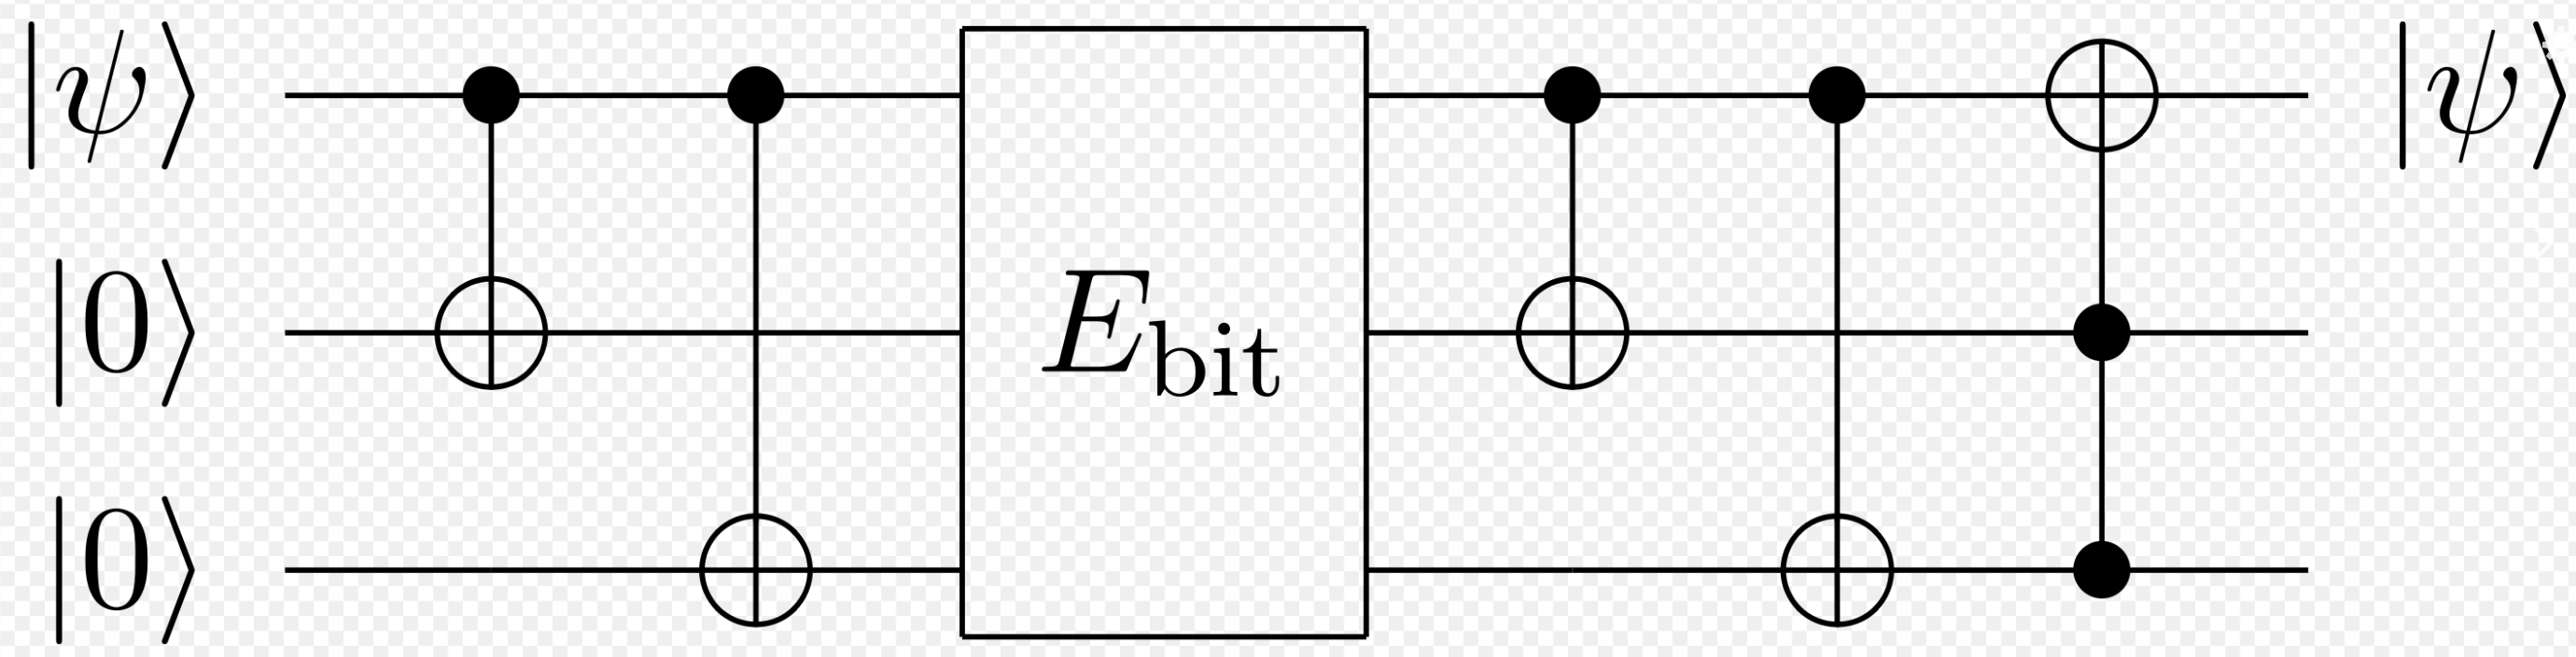
\includegraphics[width=0.98\textwidth]{Figs/QEC_BitFlipSimplified.png}
    \caption{Simplified three qubit encoder/decoder which is robust against one bit-flip noise. A control-control-not circuit swaps the first qubit if the syndrome indicates that this qubit is swapped by the channel noise \(E_{bit}\)}
\label{fig:QEC_BitFlipSimplied}
\end{figure}


\subsection{The Three qubit Phase Flip Code}
As discussed in Section 3.2, a phase flip noise can be treated as a bit flip noise if we transform an original state of the qubit in bases \(\{\ket{0}, \ket{1}\}\) to bases \(\{\ket{+}, \ket{-}\}\) by applying Hadamard operation before the channel, but applying Hadamard operation again after the channel. With this trick, the three qubit bit flip code can be used to correct a single phase flip error as well. 

This is depicted in Figure~\ref{fig:QEC_PhaseFlipSimplied}.  

The original state of the qubit 
\[\ket{\psi} = \alpha \ket{0} + \beta\ket{1}.\]

First, through the entanglement, we have 
\[\alpha \ket{000} + \beta\ket{111}.\]

Second, after the Hadamard transformation, we have
\[\alpha \ket{+++} + \beta\ket{---}.\]

The block \(E_{phase}\) introduces at most one phase-flip noise, so the output state is one of the following four states:
\begin{align*}
& \alpha \ket{+++} + \beta\ket{---}.\\
& \alpha \ket{-++} + \beta\ket{+--}.\\
& \alpha \ket{+-+} + \beta\ket{-+-}.\\
& \alpha \ket{++-} + \beta\ket{--+}.
\end{align*}

After the Hadamard transformation, we have the possible states are:
\begin{align*}
& \alpha \ket{000} + \beta\ket{111}.\\
& \alpha \ket{100} + \beta\ket{011}.\\
& \alpha \ket{010} + \beta\ket{101}.\\
& \alpha \ket{001} + \beta\ket{110}.
\end{align*}
Therefore, a syndrome decoding will correct the possible phase-flip error and return the original qubit \(\ket{\psi}\).



\begin{figure}[ht]
\centering
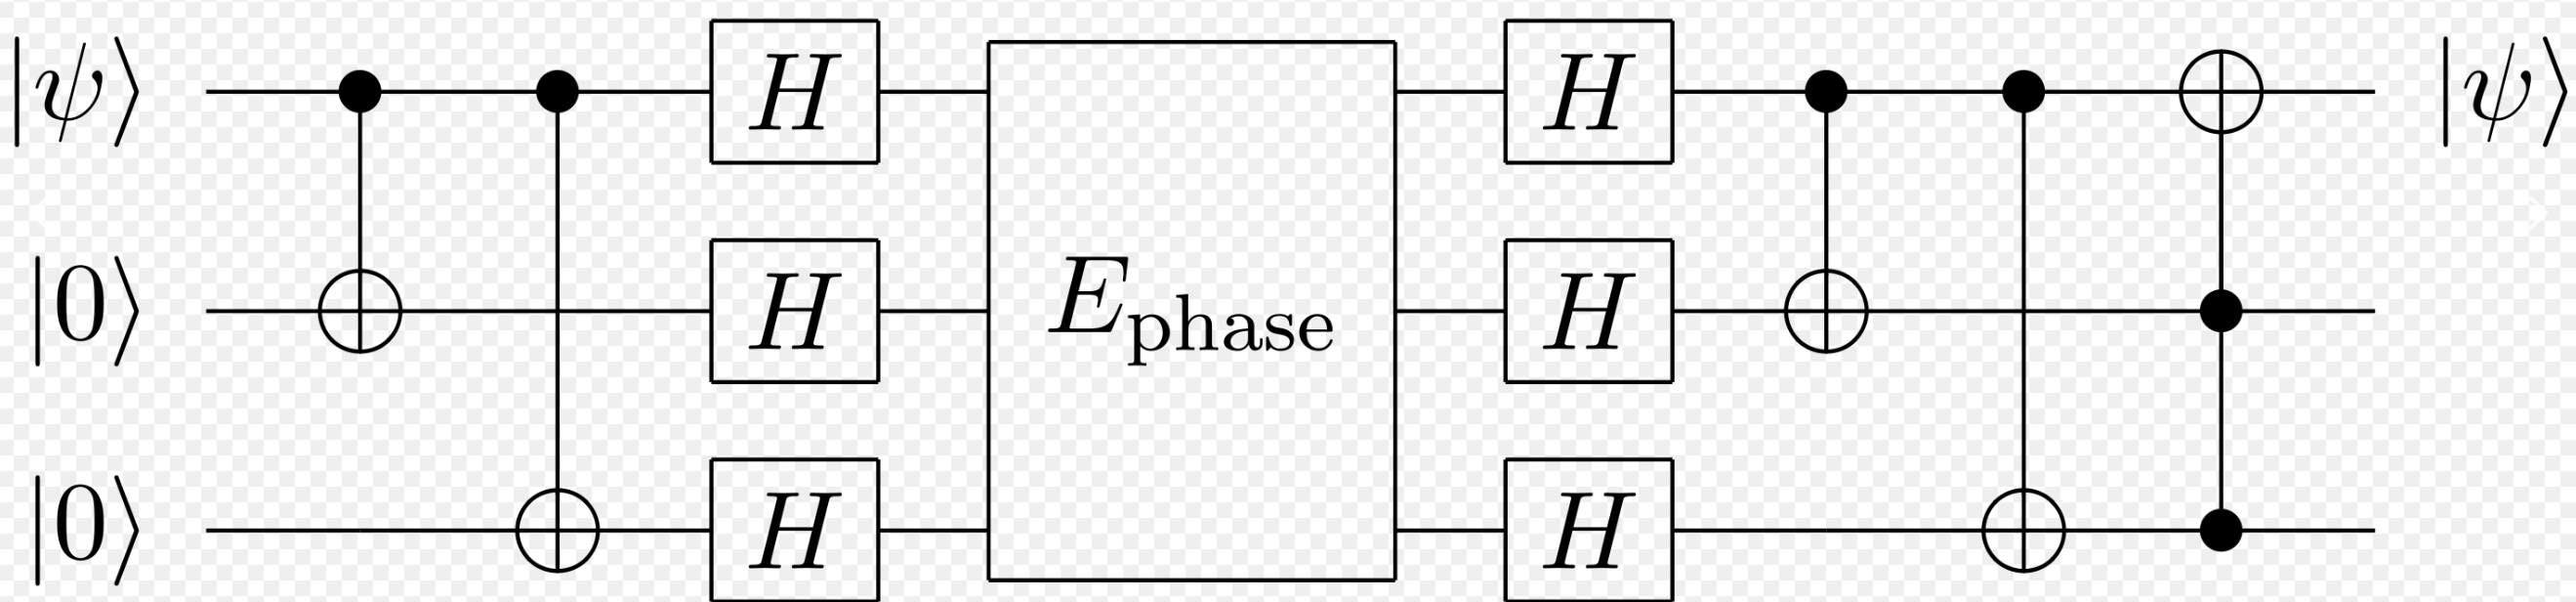
\includegraphics[width=0.9\textwidth]{Figs/QEC_PhaseFlipSimplified.png}
    \caption{Simplified three qubit encoder/decoder which is robust against one phase-flip noise. }
\label{fig:QEC_PhaseFlipSimplied}
\end{figure}



\section{Shor's Code}
Now we consider case that the error channel may induce either a bit flip, a phase flip, or both. It is possible to correct for both types of errors on any one qubit using a QEC code, which can be done using the Shor code published in 1995. This is equivalent to saying the Shor code corrects arbitrary single-qubit errors. The basic idea is to concatenate the two codes we introduced earlier: the 3 qubit code to correct a bit flip and the 3 qubit code to correct a phase flip. 

\subsection{The \(3\) qubit bit-flip code in the presence of phase-flip error}
What if we use the \(3\) qubit bit-flip code on an error channel that may have both bit-flip and phase-flip single error? 

We know that the \(3\) qubit bit-flip code guarantees to correct any single bit-flip error. If there is a phase flip error, in addition to a bit flip error, the return state could be either \(\alpha\ket{0} + \beta \ket{1}\) or \(\alpha\ket{0} - \beta \ket{1}\). That is, with the \(3\) qubit bit-flip code, such a channel becomes a channel only with phase flip error.


\subsection{Shor's code}
The code is structured as a tensor product of three structurally identical blocks. In each of the block, a qubit is first transformed by the Hadamard matrix and then entangle two ancillary \(\ket{0}\) by CNOT gate to produce 
\begin{align*}
    \ket{0} &\rightarrow \ket{000} + \ket{111}  \\
    \ket{1} &\rightarrow \ket{000} - \ket{111}  \\
    \alpha\ket{0} + \beta \ket{1} &\rightarrow \alpha(\ket{000} + \ket{111}) + \beta(\ket{000} + \ket{111})  
\end{align*}

So the total \(9\) physical qubit code for the logic qubit \(\ket{\psi} = \alpha\ket{0} + \beta \ket{1}\) is:

\begin{align}
   \alpha\ket{0} + \beta \ket{1} &\rightarrow \alpha \ket{0_S} + \beta \ket{1_S} \label{eq:ShorCode}
\end{align}
where, 
\begin{align*}
    \ket{0_S} &= \frac{1}{2\sqrt{2}}(\ket{000} + \ket{111})^{\otimes 3},\\
    \ket{1_S} &= \frac{1}{2\sqrt{2}}(\ket{000} - \ket{111})^{\otimes 3}.\\
\end{align*}

Although the circuit looks daunting, the analysis of it is simple and can be thought of a two step decoding process. 

The first step is to decode the inner \(3\) qubit code that corrects one single bit flip error in each of the \(3\) blocks. As discussed in Section 5.1, from the perspective of the logic qubits after the Hadamard matrix, the channel is equivalent to a channel with phase flip error only. 
So the whole channel now becomes a phase flip error channel and the 3 qubit code, taken as from line 1, 4, 7, can correct. 







\begin{figure}[ht]
\centering
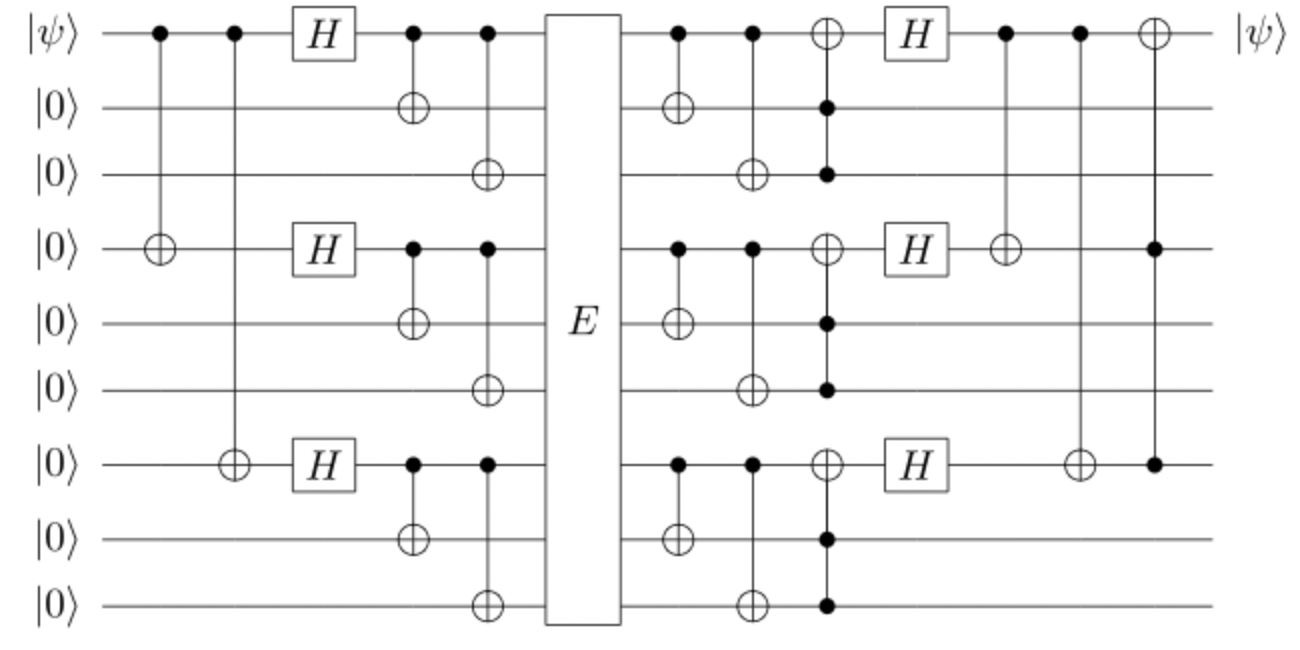
\includegraphics[width=0.9\textwidth]{Figs/QEC_ShorsCode.png}
    \caption{Shor's 9 qubit code that is robust against any single bit flip and phase flip error.}
\label{fig:QEC_Shor}
\end{figure}


\section{Exercise}
\begin{enumerate}
    \item Show the encoding part of the circuit in Fig. 4 does what it is supposed to, i.e., an initial \(\ket{+}\) is encoded as \(\ket{+++}\), and \(\ket{-}\) as \(\ket{---}\).
    
    \item Construct the code that allows correction of a \(Y\) error if it occurs on only one carrier, and design the corresponding coding and decoding circuit. [Hint: One should replace \(H\) in Fig. 4 with something else. What should it be?]
    
    \item Show that the encoding circuit in Fig. 5 produces the result in Eq.~\ref{eq:ShorCode}.

\end{enumerate}
\newpage

%\Lecturer{Hui Jin}
\Contributor{}
\LectureNumber{15}
\LectureDate{DATE}
\LectureTitle{CSS Codes and Steane Code}

\lstset{style=mystyle}


	\MakeScribeTop

%#############################################################
%#############################################################
%#############################################################
%#############################################################

\section{Introduction}
The Shor's 9-qubit code is a concatenation code structure: one repetition three code is used to deal with the bit flip noise and another repetition three code to deal with the phase flip noise. The concatenation creates a \([[9, 1, 3]]\) code, a code that encodes \(1\) logical qubit to \(9\) physical qubits, with distance three so that it can correct any single qubit error, including \(X, Y, \) or \(Z\).

This idea to use a concatenation code that an inner code deals with bit flip errors and an outer code deals with phase flip errors can be generalized. In this section, we describe a new class of quantum error-correction codes referred to as the Calderbank–Shor–Steane (CSS) codes. The construction of CSS codes is based on the use of two classical linear block codes \(C_1\) and \(C_2\). CSS code have the capability of correcting up to \(t\) bit-flip and phase-flip qubit errors, if \(C_1\) and \(C_2\) can correct \(t\) classical bit errors. But there is a caveat: not every pair of classical codes \(C_1, C_2\) can be used in a CSS construction. A necessary condition for the CSS code is the dual code of \(C_2\), namely \(C_2^{\perp}\) should be a sub-code of \(C_1\), or \(C_2^{\perp} \in C_1\). Note that this also implies that \(C_1^{\perp} \in C_2\), so at least \(C_1\) and \(C_2\) are symmetric. We will see in the next chapter why we have this requirement, using the formalization of stabilizer codes. In this chapter, we will just show that this construction works.  


I will take a top down approach in this chapter. After reviewing some of the basic results in block linear codes, we will first describe the general results of the CSS codes. Then we focus on an important instance of the CSS code, the Hadamard–Steane code, to illustrate some of the subtle details and describe how to implement the Steane code in quantum circuits. 


\section{Review of Linear Codes}
\subsection{Generator Matrix and Parity Check Matrix}
A \((n,k)\) binary linear code is generated by a basis of \(k\) vectors. It can be compactly defined either by its generator matrix or parity check matrix:  
\begin{enumerate}
    \item A generator matrix \(G\), of dimension \(n \times k\). We encode a \(k\)-bit information vector \(m\) to a \(n\)-bit codeword \(x\) by \(x = Gm\);
    \item A parity-check matrix \(H\), of dimension \(((n-k) \times n\), which satisfies \(Hx = 0\) for all codewords \(x \in C\).
\end{enumerate}
The column vector of \(G\) defines the a subspace of dimension \(k\), which produces the \(2^k\) codewords. The parity check matrix \(H\) is the null space of the subspace spanned by \(G\). That means, the row vectors of \(H\) are all orthogonal to the subspace of \(G\), or equivalently \(HG = 0\). 

We can obtain \(H\) easily from \(G\). If we write \(G\) in the systematic form,  
$$G = \begin{bmatrix}
    I_{k} \\
    P_{(n-k)\times k}
    \end{bmatrix},
$$
then the parity check matrix is:
\[H = [P_{(n-k)\times k} \; I_{n-k}].\] It is easy to see \(HG = P_{(n-k)\times k} + P_{(n-k)\times k} = 0\). That means for a codeword \(x= Gm\), we have \(Hx = HGm = 0\). 

\subsection{Dual Code}
We can define a dual code of \(C\), denoted by \(C^{\perp}\) by swapping the role of generator matrix \(G\) and parity check matrix \(H\) of the code \(C\). That is, we define a code with generator matrix \(G_{dual} = H^T\), where \(H^T\) is the transpose of \(H\). \(H^T\) has dimension \(n \times (n-k)\), therefore the encoding \(x = G_{dual} m\) encodes a \((n-k)\)-bit vector to \(n\)-bit codeword. There are \(2^{n-k}\) codewords. The parity check matrix of the dual code \(H_{dual}\) is \(G^T\). Note that the dual of \(C^{\perp}\) is \(C\). Note also that every codeword in \(C^{\perp}\) is perpendicular to every codeword in \(C\). An alternative definition of the dual code \(C^{\perp}\) is
\begin{align*}
C^{\perp} = \{b: b\cdot c = 0, \text{ for every } c in C\}. 
\end{align*}


The following lemma - Identity for linear codes and their duals - will be used later in deriving the decoding capability of CSS codes. 

\begin{lemma}
    Consider a \((n,k)\) linear code \(C\), for a \(n\)-bit vector \(z\), we have  
    \[
     \sum_{y \in C} (-1)^{y \cdot z} =
     \begin{cases}
    |C|, & \text{if } z \in C^{\perp} \\
    0.  & \text{otherwise}
    \end{cases}
    \]
\label{lemma:IdentityDual}
\end{lemma}

\begin{proof}
    If \(z \in C^{\perp}\), then \(y \cdot z = 0\) for any \(y \in C\), so \(S(z) = \sum_{y \in C} (-1)^0 = |C|. \)

    Now consider the non-trial case \(z \notin C^{\perp}\). We know the codespace \(C\) is an abelian group.  The dot product \(\phi_z(y) = y\cdot z\) is a group homomorphism\footnote{The function \(h : G(\star) \rightarrow H(\cdot)\) is a group homomorphism if whenever
\(a \star b = c\)  we have   \(h(a) \cdot h(b) = h(c).\)
In other words, the group H in some sense has a similar algebraic structure as G and the homomorphism h preserves that.
}: \(C \rightarrow Z_2\). This map is surjective when \(z \notin C^{\perp}\), which means that \(K = kernel(\phi_z(y))\) is an index two  subgroup of \(C\). The two cosets - one mapping to \(0\), the other mapping to \(1\) - have the same size. (Another way to see this is that given an element \(s \in C\) where \(\phi_z(s) = 1\), we have for any \(y \in C\) if and only \(\phi_z(y) = 0\) then \(\phi_z(y + s) = 1\), which means the whole set of codewords can be partitioned into two equal size sets whose elements are mapped to \(0\) and \(1\) respectively.) Therefore \(|K|=|C|/2\) and the result follows.

    Alternatively, the non-trial trial case \(z \notin C^{\perp}\) can be explained as the following.

    Assume \(c_0\) is one codeword in \(C\) such that \(c_0 \cdot z = 1\). Then if \(c_1\cdot z = 0\), we have \((c_0 + c_1)\cdot z = 1\);
    if \(c_1\cdot z = 1\), we have \((c_0 + c_1)\cdot z = 0\). That means the whole codewords is partitioned into two groups of equal size such that one group has \(c\cdot z = 0\) and the other group \(c \cdot z =1\) and the result follows.
    This is basically the plain language explanation of the homomorphism proof.
\end{proof}


\section{The Noise Model}
We have seen the bit-flip noise and phase-flip noise in the introduction of the quantum noise. Here we use a more compact notation. For a \(n\)-qubit \(\ket{x}\), the bit-flip noise and phase bit noise can be modeled as a bit vector \(e_X\) and \(e_Z\), such that the distorted \(n\)-qubit \(\ket{x^{\star}}\) is 
\begin{equation}
    \ket{x^{\star}} = (-1)^{x\cdot e_Z} \ket{x+e_X} \label{eq:QEC_noise}
\end{equation}
where \(x \cdot e_Z\) is the dot product of \(x\) and \(e_Z\). We use \(e_X\) to indicate the error is caused by Pauli matrix \(X\), and \(e_Z\) to indicate the error is caused by Pauli matrix \(Z\). 

For instance, \(\ket{x} = \ket{10011}, e_X = (0, 1, 0, 1, 0) \) and \(e_Z = (1, 0, 0, 1, 1)\) yield \(x \cdot eZ = 3\)  and \(x+e_X = 11001\), and the distorted state \(\ket{x^{\star}} = (-1)^3 \ket{11001} = - \ket{11001}\).

\section{Quantum Hamming Bound}
A t-error correcting quantum code is defined to be a code for which all errors of weight less than or equal to t are correctable. Since there are 3 possible single-qubit errors, the number of error operators of weight t acting on n qubits is 3tC(n,t). Therefore a t-error correcting code must be able to correct Pti=0 3iC(n,i) error operators. For nondegenerate codes, ⟨u|E1E2 |u⟩ = 0 in (31), every codeword |u⟩ and all its erroneous versions M |u⟩ must be orthogonal to every other codeword and all its erroneous versions. All these orthogonal states can only fit into the 2n-dimensional Hilbert space of n qubits if
\begin{align*}
    |C| \sum_{i=0}{t} 3^i \binom{n}{i} &\leq 2^n \\
\end{align*}
This bound is known as the quantum Hamming bound. For large \(n, t\), it becomes 
\begin{align*}
    R = k/n \leq 1 - \frac{t}{n} \log_2 3 - H(\frac{t}{n}).\\
\end{align*}
Let us plot this figure. The rate \(k/n\) falls to zero at \(\frac{t}{n} \approx 0.189\). 

Quantum Hamming bound is an upper bound. We also can derive a similar lower bound as Gilbert-Varshamov in the classical coding theory. 

\section{CSS Code}
The basic idea of CSS codes is to use a concatenation of two classical codes \(C_1\) and \(C_2\) that one is used to deal with bit flip noise and the other to deal with the phase flip noise. There is restriction on the structure of \(C_1\) and \(C_2\) to ensure that they indeed work together. 


To construct a CSS code, we require the following two conditions:
\begin{enumerate}
    \item All codewords of \(C_2^{\perp}\) belong to \(C_1\), or \(C_2^{\perp} \in C_1\); 
    \item \(C_1\) and \(C_2\) can correct \(t\) bit errors.
\end{enumerate}

Condition 1) seems hard to grasp initially. First, there seems an asymmetry present between \(C_1\) and \(C_2\).  Fortunately, it is trivial to check \(C_2^{\perp} \in C_1\) is equivalent to \(C_1^{\perp} \in C_2\) so \(C_1\) and \(C_2\) are symmetric. 

To truly understand where this condition comes from, we need to use the formalization of stabilizer codes, which we will introduce in the next chapter. For now, we will show codes with such constraints indeed work, with a touch of mystery. 

We will define codewords using the concept of cosets. So let us define that first. 

\subsection{Coset}
Given a group \(A\) and its subgroup \(B\), and its associated operator \(+\), we can define the coset of any element \(a \in A\) with respect to \(B\) as a set of elements generated by a translation of the elements in \(B\) using \(a\):
\begin{align*}
Coset(a) = \{a + b \;|\; b \in B\}.
\end{align*}
Each coset has \(|B|\) elements. Since \(B\) is a subgrop of \(A\), we have the following property:
\begin{theorem}
    For any \(x, y \in A\), either \( Coset(x)\) is identical to \(Coset(y)\), or \(Coset(x)\) does not overlap with \(Coset(y).\)
\end{theorem}

\begin{proof}
The statement is equivalent  to if \(Coset(x)\) and \(Coset(y)\) has at least one common element, then they must be identical. Let us assume \(x+b_1 = y + b_2\) is the common element, where \(x+b_1\in coset(x)\) and \(y+b_2\in coset(y)\). That means \(y-x = b_1 - b_2 \in B\) as \(b_1, b_2 \in B\). Denote \(d = y-x\). Then \(Coset(y) = \{y + b \;|\; b \in B\} = \{x + d + b \;| \;b \in B\} = {x + b' | b' \in B} = Coset(x).\)
\end{proof}

\begin{corollary}
The total number of distinct cosets is 
\[\frac{|A|}{|B|}.\]
\end{corollary}
\begin{proof}
Every element of \(A\) is in one and only one of the cosets; each coset has \(|B|\) elements which are all elements in \(A\). Therefore, there are \(\frac{|A|}{|B|}\) distinct cosets. 
\end{proof}

\subsection{Codeword Definition}
Given two linear block codes \(C_1, C_2\) satisfying the above conditions, we can construct a CSS code as follows.   First we define a quantum state \(\ket{x + y}\), for a pair of two n-bit vectors \(x, y\), where \(+\) indicates here bit-wise addition modulo \(2\). For instance, if \(x = 00101\) and \(y = 10111\), we have \(\ket{x + y} = \ket{10010}\). Now given \(x \in C_1\), we construct the the quantum state \(\ket{x + C_2^{\perp}}\) as the superposition of the Coset(x): 
\begin{align}
\ket{x + C_2^{\perp}} = \frac{1}{\sqrt{|C_2^{\perp}|}}\sum_{y \in C_2^{\perp}} \ket{x+y}.
\label{eq:QEC_CSS1}
\end{align}
The quantum state \(\ket{x + C_2^{\perp}}\) is a one-to-one map to the \(Coset(x)\); in fact, the quantum state \(\ket{x + C_2^{\perp}}\) is the normalized sum of the bases \(\ket{x+b\;|\; b \in C_2^{\perp}}\).


When the error pattern \(e_X, e_Z\) is applied to the CSS codeword \(\ket{x + C2^{\perp}}\) defined in Eq.~\ref{eq:QEC_CSS1}, the resulting distorted state is
\begin{align}
\ket{(x + C_2^{\perp})^{\star}} = \frac{1}{\sqrt{|C_2^{\perp}|}}\sum_{y \in C_2^{\perp}} (-1)^{(x+y)\cdot e_Z} \ket{x+y + e_X}.
\label{eq:QEC_CodeNoisy}
\end{align}

\subsection{Detect and Correct bit-flip noise \(e_X\)}
The first step in decoding consists of the introduction of the parity-check matrix \(H\) to correct \(e_X\). 

This is achieved by appending an n-qubit ancilla \(\ket{0}\) to \(\ket{x^{*}} = \ket{x + y + e_X}\), and passing the result through a quantum circuit that achieves the transformation \
\begin{align}
    \ket{x^{*}}\ket{0} &\rightarrow \ket{x^{*}}\ket{H x^{*}}  \label{eq:QEC_BEC} \\ 
    &= \ket{x^{*}}\ket{H(x+y) + H e_X}\nonumber\\
    &= \ket{x^{*}}\ket{H e_X}.  \nonumber 
\end{align} 
In the last step \(H(x+y)=0\) because both \(x, y\) are codewords in \(C_1\).  

The details of the quantum circuit will be describe in the Steane code example in the next section. 

Measuring each of the qubits in the ancilla \(\ket{H e_X}\) yields the syndrome vector \(H e_X\), which is common to each of the series terms in Eq.~(\ref{eq:QEC_CodeNoisy}). So the ancilla qubits are disentangled from the original qubits and can be measured without disturbing the original qubits. This syndrome measurement \(\ket{H e_X}\) will determine the error (albeit with high complexity as we are assuming here a general syndrome decoder.)
Given the error correction capability of \(C_1\), it is guaranteed that any \(t\)-error can be corrected by applying X gates in the corresponding circuit wires, the distorted \(n\)-qubit in Eq~(\ref{eq:QEC_noise}) becomes
\begin{align*}
       \ket{x^{\star}} = (-1)^{x\cdot e_Z} \ket{x}. 
\end{align*}
Therefore, the distorted state of a CSS codeword no long has the bit flip noise and gets a little cleaner, and becomes:  
\begin{align}
\ket{(x + C_2^{\perp})^{\star}}_{X} = \frac{1}{\sqrt{|C_2^{\perp}|}}\sum_{y \in C_2^{\perp}} (-1)^{(x+y)\cdot e_Z} \ket{x+y}.
\label{eq:QEC_CSSII}
\end{align}


\subsection{Detect and Correct phase-flip noise \(e_Z\)}
To correct the phase flip noise, we will first pass the X-corrected state \(\ket{(x + C_2^{\perp})^{\star}}_{X}\) through the Hadamard gate \(H^{\otimes n}\), and we get 
\begin{align}
    H^{\otimes n} \ket{(x + C_2^{\perp})^{\star}}_{X} &= \frac{1}{\sqrt{|C_2^{\perp}|}}\sum_{y \in C_2^{\perp}}  (-1)^{(x+y)\cdot e_Z} H^{\otimes n} \ket{x+y} \nonumber \\
    &= \frac{1}{\sqrt{|C_2^{\perp}|2^n}}\sum_{y \in C_2^{\perp}} (-1)^{(x+y)\cdot e_Z} \sum_{k=0}^{2^n-1} (-1)^{(x+y)\cdot k} \ket{k} \nonumber\\
    &= \frac{1}{\sqrt{|C_2^{\perp}|2^n}}\sum_{y \in C_2^{\perp}}\sum_{k=0}^{2^n-1}(-1)^{(x+y)\cdot (e_Z + k)}\ket{k} \nonumber\\
    &= \frac{1}{\sqrt{|C_2^{\perp}|2^n}}\sum_{y \in C_2^{\perp}}\sum_{k'=0}^{2^n-1}(-1)^{(x+y)\cdot k'}\ket{k' + e_Z} \nonumber\\
    &= \frac{1}{\sqrt{|C_2^{\perp}|2^n}}\sum_{k'=0}^{2^n-1}(-1)^{x\cdot k'}(\sum_{y \in C_2^{\perp}}(-1)^{y\cdot k'})\ket{k' + e_Z}\label{eq:QEC_PE}
\end{align}

By Lemma~\ref{lemma:IdentityDual}, with \(C_2\) and \(C_2^{\perp}\) swapped, we have 
\[
\sum_{y \in C_2^{\perp}}(-1)^{y\cdot k'} = 
\begin{cases}
    |C_2^{\perp}|, & \text{if } k' \in C_2\\
    0, & \text{otherwise}
\end{cases}
\]
Therefore in Eq.~(\ref{eq:QEC_PE}) the sum over \(k'\) has non-zero term if and only if  \(k' \in C_2\), so the sum  becomes 
\begin{align}
H^{\otimes n} \ket{(x + C_2^{\perp})^{\star}}_{X} &= \frac{1}{\sqrt{|C_2^{\perp}|2^n}}\sum_{k'=0}^{2^n-1}(-1)^{x\cdot k'}(\sum_{y \in C_2^{\perp}}(-1)^{y\cdot k'})\ket{k' + e_Z} \nonumber \\
&= \frac{1}{\sqrt{|C_2^{\perp}|2^n}}\sum_{k'\in C_2}(-1)^{x\cdot k'} |C_2^{\perp}| \ket{k' + e_Z} \nonumber\\
&= \sqrt{\frac{|C_2^{\perp}|}{2^n}}\sum_{k'\in C_2}(-1)^{x\cdot k'} \ket{k' + e_Z} \label{eq:QEC_PEC}
\end{align}

At this point, we effectively turned the phase flip error to a bit flip error. The use of Hadamard matrix to achieving this is in principle the same as in the Shor's 9-bit code. Now we can use the same technique as in Eq.~\ref{eq:QEC_BEC}, to correct the error \(e_Z\), by using the parity check matrix of code \(C_2\) to obtain the syndrome. By construction, \(C_2\) can correct \(t\) errors. 

After correction, we obtain
\begin{align*}
\sqrt{\frac{|C_2^{\perp}|}{2^n}}\sum_{k'\in C_2}(-1)^{x\cdot k'} \ket{k'}, 
\end{align*}
which corresponds to the Hadamard transform of the original codeword: \[H^{\otimes n} \ket{(x + C_2^{\perp})}.\]
Applying Hadamard transformation again inverts back to the original codeword \(\ket{(x + C_2^{\perp})}\). 

\section{Steane Code}
In this section, we describe an important instance of a CSS code, the Steane code. It is based on our familiar Hamming code \(C_1 = (7, 4)\), and its dual \(C_2 = C^{\perp}\). 


The Steane code has the same bit-flip and phase-flip error correction capability as the earlier-described Shor 9-bit repetition code, namely, up to one error in either or both cases, but it uses \(7\)-qubit codewords, thus more efficient than the Shor's code. The best code to achieve the same capability uses \(5\)-qubit. 

\subsection{The definition of \(C_1\) and \(C_2\)}

\(C_1\) is the \(7,4,3)\) Hamming code. It is able to correct \(1\) (classical) bit error. The generator matrix \(G\) of \(C_1\) is: 
$$G = \begin{bmatrix}
    1 & 0 & 0 & 0\\
    0 & 1 & 0 & 0\\
    0 & 0 & 1 & 0\\
    0 & 0 & 0 & 1\\
    0 & 1 & 1 & 1\\
    1 & 0 & 1 & 1\\
    1 & 1 & 0 & 1
\end{bmatrix}$$
A codeword in \(C_1\) is generated by \(c = Gm\), where message \(m\) is a length-4 column vector.

The corresponding parity check matrix \(H\) of \(C_1\) is:  
$$H = \begin{bmatrix}
    0 & 0 & 0 & 1 & 1 & 1 & 1\\
    0 & 1 & 1 & 0 & 0 & 1 & 1\\
    1 & 0 & 1 & 0 & 1 & 0 & 1
\end{bmatrix}$$
where a length-7 column vector \(c\) is a codeword iff \(Hc= 0.\) By construction, \(HG=0\), ie the row vectors of \(H\) defines the null space of the subspace defined by the column vectors of \(G\).


\(C_2\) is the dual code of \(C_1\). A dual code of \(C_1\) simply means that we use the transpose of parity check matrix \(H^T\) of \(C_1\) as the generator matrix of \(C_2\):
$$G_{dual} = \begin{bmatrix}
    0 & 0 & 1\\
    0 & 1 & 0\\
    0 & 1 & 1\\
    1 & 0 & 0\\
    1 & 0 & 1\\
    1 & 1 & 0\\
    1 & 1 & 1
\end{bmatrix}$$
A codeword in \(C_2\) is generated by \(c = G_{dual} m\), where message \(m\) is a length-3 column vector. 


\begin{lemma}
    All codewords in \(C_2\) belong to \(C_1\). 
\end{lemma}

\begin{proof}
We will show that any codeword \(c\) in \(C_2\) is also in \(C_1\) by showing \(Hc = 0\). A codeword \(c\) in \(C_2\) can be written as \(c = G_{dual} m = H^T m\). Therefore \(Hc = H H^T m\). Notice that the row vectors of \(H\) are orthogonal to each other, so \(H H^T = 0\) and the results follows. 
\end{proof}

Now since \(C_2\) is the dual of \(C_1\), the dual of \(C_2\) is \(C_1\), ie. \(C_2^{\perp} = C_1\).

Thus, based on the construction, \(C_1\) and \(C_2\) has the following property: 

\begin{enumerate}
    \item All codewords of \(C_2\) belong to \(C_1\); 
    \item \(C_1\) and \(C_2^{\perp}\) are the same \((7,4,3)\) Hamming code, which can correct \(1\) bit error.
\end{enumerate}

So the Steane code satisfies the conditions specified in the CSS code requirement and is able to correct bit flip and/or phase flip on a single bit. 

\subsection{A Compact way to represent the codewords of \(C_2\)}
The parity check matrix of \(C_2\) is \(H_{dual} = G^T\):
$$H_{dual} = \begin{bmatrix}
    1 & 0 & 0 & 0 & 0 & 1 & 1 \\
    0 & 1 & 0 & 0 & 1 & 0 & 1 \\
    0 & 0 & 1 & 0 & 1 & 1 & 0 \\
    0 & 0 & 0 & 1 & 1 & 1 & 1
\end{bmatrix}$$
Based on this, the parity bits based the three message bits \(m_1, m_2, m_3\) are 
\begin{align*}
    p_1 &= m_2 + m_3 \\
    p_2 &= m_1 + m_3 \\
    p_3 &= m_1 + m_2 \\
    p_4 &= m_1 + m_2 + m_3 
\end{align*}
Thus three messages bits \(m_1, m_2, m_3\) is encoded to 
\begin{align}
code(m_1, m_2, m_3) = (m_2 + m_3, m_1 + m_3, m_1 + m_2, m_1 + m_2 + m_3, m_1, m_2, m_3)
\label{eq:QEC_HammingDualEncode}
\end{align}

We can list the 8 codewords: 
\begin{align*}
    0000000,  1101001, & 1011010, 0110011 \\
    0111100,  1010101, & 1100110, 0001111 \\
\end{align*}

\subsection{The Steane Codeword}
There are \(\frac{|C_1|}{|C_2|} = \frac{2^4}{2^3} = 2\) codewords in the Steane code. They are the two following cosets, denoted by logit qubits \(\ket{\hat{0}}\), and \(\ket{\hat{1}}\):
\begin{align*}
    \ket{\hat{0}} &= \ket{0000000 + C_2} \\
    \ket{\hat{1}} &= \ket{1111111 + C_2}  
\end{align*}
Expanding the above codeword into bases, and using the fact how the codewords are generated from the message bits Eq.~(\ref{eq:QEC_HammingDualEncode}), we have 
\begin{align}
\ket{\hat{0}} &= \ket{0000000 + C_2} \nonumber\\
&\defeq \frac{1}{\sqrt{8}}\sum_{c\in C_2}\ket{0000000 + c} \nonumber\\
&= \frac{1}{\sqrt{8}} (\ket{0000000} + \ket{1101001} + \ket{1011010} + \ket{0110011} + \nonumber \\ 
 &\;\;\;\;\;\;\;\;\;\;\ket{0111100}  + \ket{1010101}  + \ket{1100110} + \ket{0001111}) \nonumber \\
 &= \frac{1}{\sqrt{8}} \sum_{m_1,m_2,m_3}\ket{m_2 + m_3}\ket{m_1 + m_3}\ket{m_1 + m_2} \ket{m_1 + m_2 + m_3}\ket{m_1}\ket{m_2}\ket{m_3} \label{eq:QEC_SteaneSum1}
\end{align}

Similarly, 
\begin{align}
\ket{\hat{1}} &=  \ket{111111 + C_2} \nonumber\\
  &=\frac{1}{\sqrt{8}}\sum_{m_1,m_2,m_3}\ket{m_2 + m_3+1}\ket{m_1 + m_3 + 1}\ket{m_1 + m_2+1} \otimes \nonumber\\
   & \;\;\;\;\;\;\;\;\;\ket{m_1 + m_2 + m_3+1} \ket{m_1+1}\ket{m_2+1}\ket{m_3+1} \nonumber\\
   &= \frac{1}{\sqrt{8}} \sum_{m_1^{'},m_2^{'},m_3^{'}}\ket{m_2^{'} + m_3^{'}+1}\ket{m_1^{'} + m_3^{'} + 1}\ket{m_1^{'} + m_2^{'}+1} \otimes \nonumber\\
   &\;\;\;\;\;\;\;\;\;\ket{m_1^{'} + m_2^{'} + m_3^{'}} \ket{m_1^{'}}\ket{m_2^{'}}\ket{m_3^{'}} \label{eq:QEC_SteaneSum2}
\end{align}
We replace \(m_i + 1\) by \(m_i^{'}\) in the last step.  

The Eqs~(\ref{eq:QEC_SteaneSum1}) and (\ref{eq:QEC_SteaneSum2}) can be combined to one encoding logic for logit qubit \(\ket{a}\): 
\begin{align}
\ket{\hat{a}} &=\frac{1}{\sqrt{8}} \sum_{m_1,m_2,m_3}\ket{m_2 + m_3+a}\ket{m_1 + m_3 + a}\ket{m_1 + m_2+a} \ket{m_1 + m_2 + m_3} \ket{m_1}\ket{m_2}\ket{m_3} \label{eq:QEC_SteaneSum}     
\end{align}


\subsection{The Quantum Circuit for the Steane Code}

The key element in the quantum circuit to implement the Steane code is how to realize the summation in Eq.~(\ref{eq:QEC_SteaneSum}). 

Our powerful Hadamard transforms does something similar to Eq~\ref{eq:QEC_SteaneSum1} already,  
\[H^{\otimes 3}\ket{0}^{\otimes 3} =\frac{1}{\sqrt{2^3}} 
\sum_{m_1,m_2, m_3} \ket{m_1}\ket{m_2}\ket{m_3}.\]
What we are missing are the qubits corresponding to the parity bits. How do we get these? 

Let us analyze an elementary circuit in  Figure~\ref{fig:QEC_SteaneSimple}.
 
 \begin{figure}[h]
    \centering
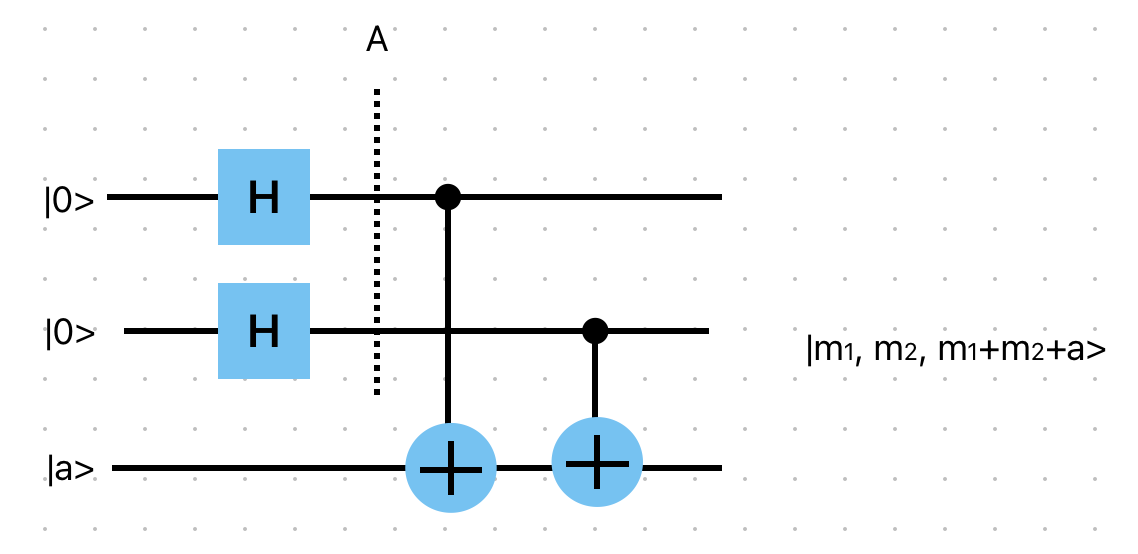
\includegraphics[width=0.6\textwidth]{Figs/Steane_simple.png}
    \caption{An elementary circuit to generate a code with a simple parity.}
    \label{fig:QEC_SteaneSimple}
\end{figure}

It is seen from the figure that the two Hadamard gates produce \(\ket{+}^{\otimes 2}\) at the place indicated by "A", which is \[\sum_{m_1,m_2} \ket{m_1}\ket{m_2} = \frac{1}{2}(\ket{00} + \ket{01} + \ket{10}+ \ket{11}.\] They act as control qubits on the target qubit \(\ket{a}\)  through CNOT gates. This circuit generate a simple code where logic qubit \(\ket{a}\) is mapped to the codeword: 
\[\frac{1}{2} 
\sum_{m_1,m_2} \ket{m_1}\ket{m_2}\ket{m_1+m_2+a}.\]


We first observe that \(\ket{a}\), which represents the originator’s message qubit to be encoded, is not limited to the basis states \(\ket{0}\) or \(\ket{1}\); rather, by linearity, the encoding also works for general qubit \(\ket{a} = \alpha\ket{0} + \beta\ket{1}\).

Based on the same principle, we can draw the quantum circuit to generate the Steane code as the sum in Eq.~(\ref{eq:QEC_SteaneSum}). 

 \begin{figure}[h]
    \centering
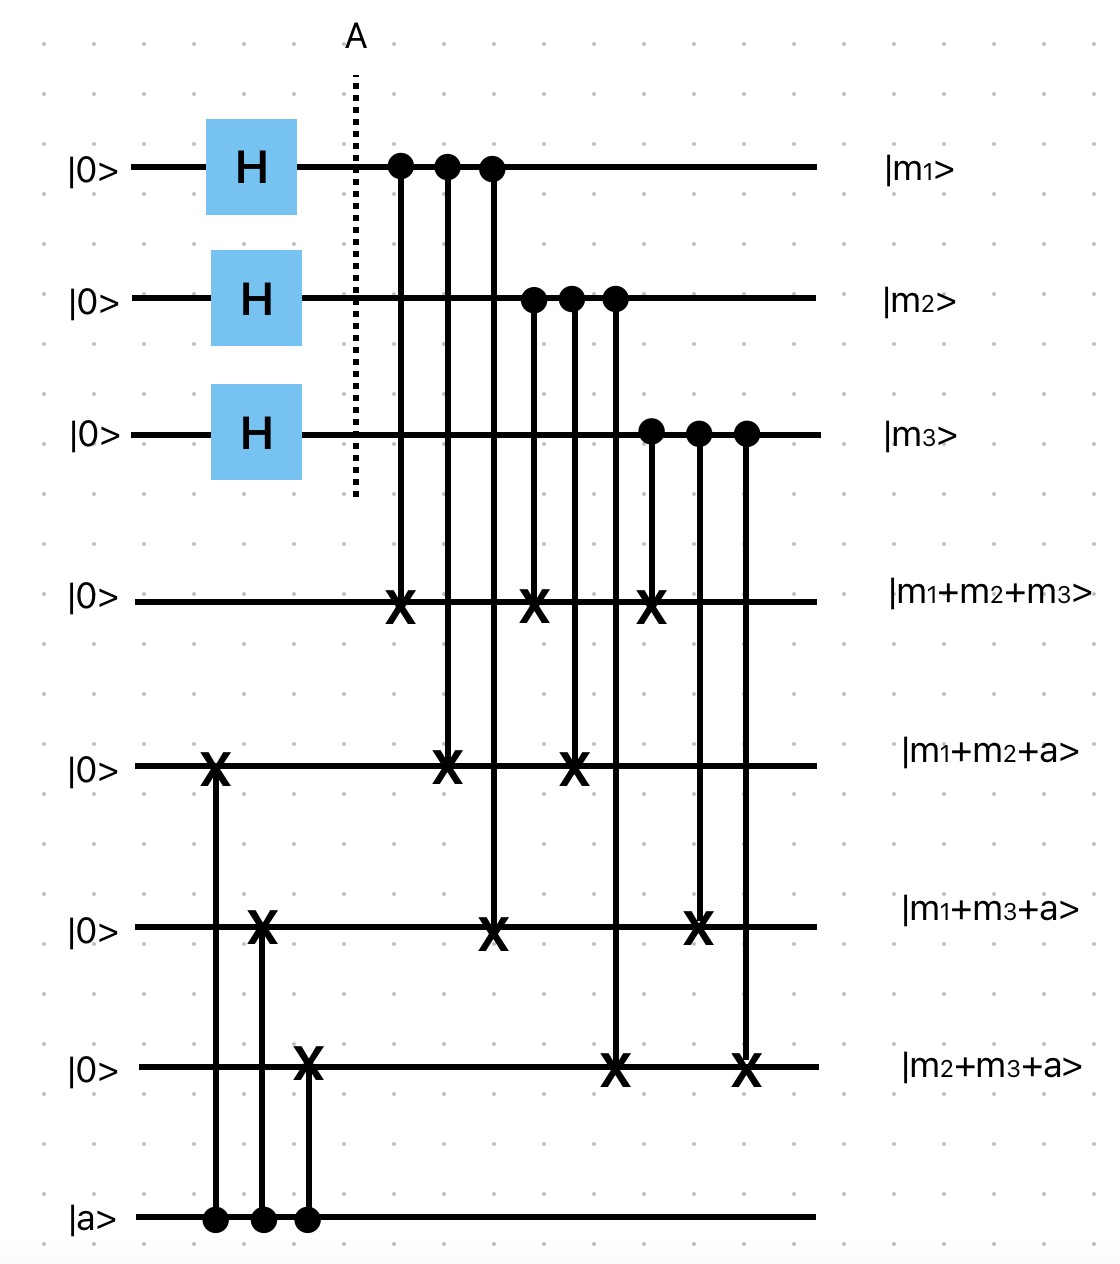
\includegraphics[width=0.7\textwidth]{Figs/Steane_FullCode.png}
    \caption{The quantum circuit to realize Steane code.}
    \label{fig:QEC_SteaneFullCode}
\end{figure}


\section{Intuition on Syndrome Extraction}
The syndrome extraction operation is
\begin{align}
XOR^{(H)}_{q,a}(\ket{0}_a \ket{u+e})= \ket{H eT}_a \ket{u+e} 
\end{align}
The fact that the classical syndrome is independent of the message is now highly significant, for if the initial state of q is any superposition \(\sum_{u in C} a_u \ket{u}\), the syndrome extraction does not leave \(q\) and \(a\) entangled:
\begin{align*}
XOR^{(H)}_{q,a}(\ket{0}_a X_e \sum_{u in C} a_u \ket{u} =\ket{H eT}_a \sum_{u \in C} a_u \ket{u+e}
\end{align*}
Recovery is completed by measuring \(a\), deducing \(e\) from \(HeT\), and applying \(X_e\) to \(q\).

\section{Exercises}
\begin{enumerate}
    \item Prove the dual code theorem. 
    \begin{align*}
        H^{\otimes n} \sum_{i \in C} \ket{i} = \sum_{i \in C^{\perp}} \ket{i}.
    \end{align*}
\end{enumerate}
\newpage

%\Lecturer{Hui Jin}
\Contributor{}
\LectureNumber{15}
\LectureDate{DATE}
\LectureTitle{CSS Codes and Steane Code}

\lstset{style=mystyle}


	\MakeScribeTop

\section{Stabilizer Codes Introduction}

A \emph{stabilizer code} is a quantum error-correcting code described by an abelian subgroup
\(\mathcal{S}\) of the (n)-qubit Pauli group \(\mathcal{P}_n\). The code space is the joint
(+1)-eigenspace of all operators in \(\mathcal{S}\).

\subsection*{Pauli group}
The (n)-qubit Pauli group \(\mathcal{P}_n\) is generated by tensor products of the single-qubit operators
\[
I = \begin{pmatrix}1 & 0 \ 0 & 1\end{pmatrix}, \quad
X = \begin{pmatrix}0 & 1 \ 1 & 0\end{pmatrix}, \quad
Y = \begin{pmatrix}0 & -i \ i & 0\end{pmatrix}, \quad
Z = \begin{pmatrix}1 & 0 \ 0 & -1\end{pmatrix},
\]
together with global phases \({\pm 1, \pm i}\).

\subsection*{Stabilizer group}
A stabilizer code is defined by an abelian subgroup \(\mathcal{S} \subset \mathcal{P}_n\), not containing \(-I\).
Each \(S \in \mathcal{S}\) imposes the constraint
\[
S , |\psi\rangle = |\psi\rangle, \quad \forall S \in \mathcal{S}.
\]

If \(\mathcal{S}\) is generated by \(n-k\) independent elements, then the code space has dimension \(2^k\). Such a code is called an \([[n,k,d]]\) code.

\subsection*{Error detection and correction}
Errors are modeled as Pauli operators \(E \in \mathcal{P}_n\).
\begin{itemize}
\item If \(E\) commutes with all stabilizers, it preserves the code space and acts as a logical operator.
\item If \(E\) anticommutes with some stabilizer, measurement of that stabilizer yields eigenvalue \(-1\).
\end{itemize}

The pattern of \(\pm 1\) outcomes is called the \emph{syndrome}, which identifies the error up to equivalence.

The minimum weight of a Pauli operator that maps one valid codeword to another (without being in \(\mathcal{S})\) is the \emph{distance} \(d\). An \([[n,k,d]]\) stabilizer code corrects up to \(\lfloor (d-1)/2 \rfloor\) errors.

\subsection*{CSS construction}
A special class of stabilizer codes, due to Calderbank--Shor and Steane (CSS codes), arises from pairs of classical binary linear codes \((C_X, C_Z)\) with
\[
C_Z^\perp \subset C_X.
\]

Here,
\begin{itemize}
\item \(Z\)-type stabilizers are defined from parity checks of \(C_Z\),
\item \(X\)-type stabilizers from parity checks of \(C_X\).
\end{itemize}

The Steane code \([[7,1,3]]\) is a canonical example of this construction.


\section{Steane code in Stabilizer Formulation}
In the CSS construction of the Steane code, each row \(h \in H\) of the parity-check matrix defines both a \(Z\)-type stabilizer \(Z^h\) and an \(X\)-type stabilizer \(X^h\).

\[
X^h = \bigotimes_{i=1}^7 X^{h_i},
\qquad
Z^h = \bigotimes_{i=1}^7 Z^{h_i},
\]
where \(h=(h_1,\dots,h_7)\).

---

\subsection{Action on basis states}

For a computational basis state \(|v\rangle\), with \(v\in {0,1}^7\),
\[
X^h |v\rangle = |v \oplus h\rangle,
\]
where \(\oplus\) is bitwise XOR.

Thus, an \(X\)-stabilizer does not leave \(|v\rangle\) invariant; it maps it to another basis state shifted by \(h\).

---

\subsection{Stabilizer condition}

If a state \(|\psi\rangle\) is stabilized by \(X^h\),
\[
X^h |\psi\rangle = |\psi\rangle,
\]
then whenever \(|v\rangle\) has nonzero amplitude in \(|\psi\rangle\), the shifted state \(|v\oplus h\rangle\) must also appear with the same amplitude. Hence, the amplitudes are constant on orbits generated by the shifts \(h\).


\subsection{Consequence for CSS codes}

\begin{itemize}
\item Z stabilizers: restrict the support to classical codewords \(C = \ker(H)\).
\item X stabilizers: enforce uniform superpositions across cosets generated by \(C^\perp\).
\end{itemize}


For the Steane code, where \(C_X = C_Z = C\) (the Hamming \([7,4,3]\) code), the result is:
\begin{itemize}
    \item \(|0_L\rangle\) is the equal superposition of the 8 codewords of \(C\),
    \item \(|1_L\rangle = X^{\otimes 7}|0_L\rangle\) is the equal superposition of the complementary coset.
\end{itemize}
Thus, the \(Z\)-part selects the codewords, while the \(X\)-part forces them to appear with equal weight.

\newpage

%\Lecturer{Hui Jin}
\Contributor{}
\LectureNumber{16}
\LectureDate{DATE}
\LectureTitle{Stabilizer Codes and Quantum LDPC Codes}

\lstset{style=mystyle}


	\MakeScribeTop

%#############################################################
%#############################################################
%#############################################################
%#############################################################
\section{Revisiting the Shor's code}
[Credit: This chapter refers a lot from Steane's "A Tutorial on Quantum Error Correction"]

Let us look more closely at the procedure we used to correct errors for the Shor's nine-qubit code. Let us assume the logical qubits are \(\ket{0}_S\) and \(\ket{1}_S\) and the original qubit is encoded as \(\ket{\psi} = \alpha \ket{0}_S + \beta \ket{1}_S\). We assume \(E\ket{\psi}\) is the noisy version before decoding. 

To detect a bit flip error on one of the first three qubits, we compared the first two qubits and the first and third qubits. This is equivalent to measuring the eigenvalues of \(Z_1Z_2\) and \(Z_1Z_3\).

If the first two qubits are the same, the eigenvalue of \(Z_1Z_2\) is \(+1\); if they are different, the eigenvalue is \(-1\). Similarly, to detect a phase error, we compare the signs of the first and second blocks of three and the first and third blocks of three. This is equivalent to measuring the eigenvalues of \(X_1X_2X_3X_4X_5X_6\) and \(X_1X_2X_3X_7X_8X_9\). Again, if the signs agree, the eigenvalues will be \(+1\); if they disagree, the eigenvalues will be \(-1\). In order to totally correct the code, we must measure the eigenvalues of a total of eight operators, which are \(\{M_1 = Z_1Z_2, M_2 = Z_1Z_3, M_3 = Z_4Z_5, M_4 = Z_4Z_6, M_5 = Z_7Z_8, M_6 = Z_7Z_9, M_7 = X_1X_2X_3X_4X_5X_6, M_8 = X_1X_2X_3X_7X_8X_9\}\). 

Codewords are  eigenvectors of all eight of these operators with eigenvalue \(+1\). Since we start with the vector space of dimension \(2^9\), and there are eight operators, each dividing the space by half, the codespace has dimension of \(2^1\), there are two valid codewords \(\ket{0}_S\) and \(\ket{0}_S\). 

All the operators that fix both \(\ket{0}_S\) and \(\ket{0}_S\) can be written as the product of these eight operators. The set of operators that fix \(\ket{0}_S\) and \(\ket{0}_S\) form a group \(S\), called the stabilizer of the code, and the above eight operators are the generators of this group.


When we measure the eigenvalue of \(M_1\), we determine if a bit flip error has occurred on qubit one or two, i.e., if \(X_1\) or \(X_2\) has occurred. Note that both of these errors anti-commute with \(M_1\), while \(X_3\) through \(X_9\), which cannot be detected by just \(M_1\), commute with it. Similarly, \(M_2\) detects \(X_1\) or \(X_3\), which anti-commute with it. Similarly \(M_7\) detects a phase flip error among the first six qubits, namely the possibly single errors  \(Z_1, Z_2, Z_3, Z_4, Z_5,\) or \(Z_6\). In general, if \(M \in S, \{M,E\} = 0\), and \(\ket{\psi}\) in the codespace, then
\begin{align*}
    ME \ket{\psi}  = - EM \ket{\psi} = -E\ket{\psi},
\end{align*}
so \(E \ket{\psi}\) is an eigenvector of \(M\) with eigenvalue \(-1\) instead of \(+1\) and to detect \(E\) we need only measure \(M\).

\section{Stabilizer Codes}
We will now examine the mathematics of error operators and syndromes, using the insightful approach put forward by Gottesman  and Calderbank et. al. This introduced the concept of the stabilizer, which yielded great insights into quantum error correction codes, and changed the approach from studying the code itself to studying the error operators. 

Consider the set \(\{I, X, Y, Z\}\) consisting of the identity plus the three Pauli operators. The Pauli operators all square to \(I\): \(X^2 = Y^2 = Z^2 = I\), and have eigenvalues \(\pm 1\). Two members of the set only ever commute  or anticommute. Tensor products of Pauli operators, i.e. error operators, also square to one and either commute or anticommute. 


\subsection{Error Vectors for error operators}
If there are \(n\) qubits in the quantum system, then error operators will be of length \(n\). We know any error operator can be regarded as a tensor product of the Pauli operators. In particular, any error operator can be decomposed as a product of an \(X\) error vector and an \(Z\) error vector. For example, error vector \(X\otimes I\otimes Z \otimes Y \otimes X\) can be written as \(X\otimes I\otimes I \otimes X \otimes X\) times \(I\otimes I\otimes Z \otimes Z \otimes I\). We define \(X_{iX}\) to be the \(X\) error vector, where \(iX\) is an \(n\)-bit vector that the \(k\)-th position is \(1\) if and only the \(k\)-th position of the \(X\) error vector is \(X\); similarly we define \(Z_{iZ}\) to be the \(Z\) error vector. For example, \(X_{10011}\) is the error vector representing \(X\otimes I\otimes I \otimes X \otimes X\).

The weight of an error operator is sum of the Hamming weight of \(iX\) and Hamming weight of \(iZ\). For example \(X_{10011}Z_{00110}\) has length \(5\), weight \(4\).

Any \(X\) vector commutes with another \(X\) vector, as any \(Z\) vector commutes with another \(Z\) vector. When does an \(X\) vector commutes with an \(Z\) vector? We can state it cleanly using the error vector notation. 
\begin{lemma}
    \[X_{iX} Z_{iZ} = Z_{iZ} X_{iX} \;\; \text{if and only if }\;\; iX\cdot iZ = 0\]
    \label{lemma:Stable}
\end{lemma}

Let \(H = \{M\}\) be a set of commuting error operators. Since the operators all commute, they can have simultaneous eigenstates. This is necessary and sufficient. It is necessary as if two operators \(\{E, F\}\) have simultaneous eigenstate \(\ket{\psi}\), then:
\begin{align*}
    & EF\ket{\psi} = E\ket{\psi} = \psi = FE\ket{\psi} \\
 \Rightarrow & (EF-FE)\ket{\psi} = 0 \\
    & E,\; F \;\; \text{commute}
\end{align*}


Let \(C = \{\ket{u}\}\) be an orthonormal set of simultaneous eigenstates all having eigenvalue \(+1\):
\begin{align*}
M\ket{u}=\ket{u}  u \in C,  M \in H.    
\end{align*}

The set C is a quantum error correcting code, and H is its stabilizer. 

The orthonormal states \(\ket{u}\) are termed code vectors or quantum codewords. We further assume \(H\) is a group. Its size is \(2^{n-k}\), and it is spanned by \(n-k\) linearly independent members of \(H\). In this case \(C\) has \(2^k\) members, so it encodes \(k\) qubits, 
since its members span a \(2^k\) dimensional subspace of the \(2^n\)
dimensional Hilbert space of the whole system. A general state in this subspace, called an encoded state or logical state, can be expressed as a superposition of the code vectors:
\begin{align*}
\ket{\phi}_L = \sum_{u \in C} a_u \ket{u}    
\end{align*}


Naturally, a given QECC does not allow correction of all possible errors. Each code allows correction of a particular set S = {E} of correctable errors. The task of code construction consists of finding codes whose correctable set includes the errors most likely to occur in a given physical situation. We will turn to this important topic in the next section. First, let us show how the correctable set is related to the stabilizer, and demonstrate how the error correction is actually achieved.

\subsection{Harmless Errors, Detectable Errors, and Undetectable Errors: the Good, Bad, and Ugly}
Using the stabilizer formalization, we can categorize different error operators afflicted by the computation environment.

Suppose \(E\) commutes with some \(M \in H\), so that
\(ME\ket{\psi} = EM \ket{\psi} = E \ket{\psi}\). \(E\ket{\psi}\) is a \(+1\) eigenvector of \(M\), so \(E\) is not detected as an error from stabilizer element \(M\). Conversely, suppose \(E\) and \(M\) anticommute so \(E\ket{\psi}\) is a \(-1\) eigenvector of \(M\). Then \(E\) is detected as an error.


Let \(N(S)\) be the set of operators \(N\) which commute with all \(M\in H\). A stabilizer code detects errors outside of \(N(S) \ S\) because errors outside of \(N(S)\) anticommute with stabilizers and are detected by measuring eigenvalues. These are the \textbf{Bad} errors. Errors in \(H\) act like the identity by definition - they are trivial errors, or the \textbf{Good} errors. While the errors in \(N(S) \ S\) cannot be detected - they are the \textbf{Ugly} ones.


Define the weight of a code to be the minimum of the set of weights of the elements of \(N(S) \ S\). The weight of a code is the weight of the smallest error it cannot detect.

\subsection{Error Correcting}
Correcting error requires us to know exactly which operator had its eigenvalues change, so that we can apply the proper recovery procedure. We do this by measuring the eigenvalues of every operator in the stabilizer and noting that they can change differently due to different errors. For instance, an error that commutes with the first generator but not the second will give eigenvalues of \(+1\) and \(-1\); these will be flipped for the opposite commutation.

It can be shown that \(E\) and \(F\) have the same error syndrome (eigenvalue measurements) if and only \(E^{\dagger} F \in N(S)\). Then if \(E^{\dagger} F \notin N(S)\), \(E\) and \(F\) may be distinguished by their different error syndromes. Meanwhile, if \(E^{\dagger} F \in S\), then \(E\ket{\psi} = F\ket{\psi}\), and we cannot distinguish between the two errors but don’t need to because they do the same thing to the codewords. Then a stabilizer code corrects errors for which \(E^{\dagger} F \notin N(S) \ S\) for all possible pairs of errors \((E,S)\).


\section{CSS stabilizers}
For CSS code, the error operators in the stabilizers \(H\) can be partitioned into two subgroups pure \(X\) operators and \(Z\) operators, denoted by \(H_X\) and \(H_Z\). Elements of \(H_X\) correct bit flip errors and elements of \(H_Z\) correct phase flip errors.  

\(H_X\) is constructed from the parity check matrix of one classical code \(C_1\). Specifically, in that parity check matrix, each row corresponds to an error operator by replacing the "1" as \(Z\) and "0" as \(I\). (Bit flip errors are detected and corrected by \(Z\) operators). Assume \(C_1\) is \((n, k_1, d_1)\) code, then \(H_X\) has \(n-k_1\) elements. The error vector for each error operator is simply the binary vector corresponding row. 

Similarly, \(H_Z\) is constructed from the parity check matrix of another classical code \(C_2\). Specifically, in that parity check matrix, each row corresponds to an error operator by replacing the "1" as \(X\) and "0" as \(I\). (Bit flip errors are detected and corrected by \(X\) operators). Assume \(C_2\) is \((n, k_2, d_2)\) code, then \(H_Z\) has \(n-k_2\) elements. The error vector for each error operator is simply the binary vector corresponding row. 

The concatenated code has total \((n-k_1 + n - k_2) = 2n - (k_1 + k_2)\) constraints, so the code dimension is \([[n, k_1 + k_2 -n, \text{min}(d_1, d_2)]]\).

Elements in \(H_X\) commute, so do the elements in \(H_Z\). For a pair element \(X_{iX} \in H_X\) and \(Z_{iZ} \in H_Z\) to commute, we need \(iX\cdot iZ = 0\), where \(iX, iZ\) are the error vectors, as stated in Lemma \ref{lemma:Stable}.  


Let us now illustrate the Steane code in this new formalization.


\section{The Error Operator On Codewords}
\newpage


\end{document}

\newpage

\input{appx/notation}


\end{document}
